\chapter{关于本模板}

本模板根据浙江大学研究生院编写的《浙江大学研究生学位论文编写规则》~\cite{zjugradthesisrules},
在原有的 zjuthesis 模板~\cite{zjuthesis}基础上开发而来。

本模板的本科生版本\cite{zjuthesisrules}得到了浙江大学本科生院老师的支持与审核,
已经在本科生院网上公示。
但当前的研究生版本并未经过研究生院老师的审核,
同学们使用时要注意对照模板与要求,
切不可盲目使用。

作者本人并未编写过浙江大学研究生毕业论文,
所以不清楚具体要求。
如果有热心同学愿意帮忙,
可以替我联系相关老师,我会配合审核并修改代码。

\section{Overleaf 使用注意事项}

如果你在Overleaf上编译本模板,请注意如下事项:

% \begin{itemize}
%     \item 删除根目录的 ``.latexmkrc'' 文件,否则编译失败且不报任何错误
%     \item 字体有版权所以本模板不能附带字体,请务必手动上传字体文件,并在各个专业模板下手动指定字体。
%         具体方法参照 GitHub 主页的说明。
%     \item 当前的Overleaf默认使用TexLive 2017进行编译,但一些伪粗体复制乱码的问题需要TexLive 2019版本来解决。
%         所以各位同学可以在Overleaf上编写论文时务必切换到TexLive 2019或更新版本来编译,以免产生查重相关问题。
%         具体说明参照 GitHub 主页。
% \end{itemize}


\section{节标题}

我们可以用includegraphics来插入现有的jpg等格式的图片,
如\autoref{fig:zju-logo}所示。

\begin{figure}[htbp]
    \centering
    \includegraphics[width=.3\linewidth]{logo/zju}
    \caption{\label{fig:zju-logo}浙江大学LOGO}
\end{figure}


\subsection{小节标题}


\par 如\autoref{tab:sample}所示,这是一张自动调节列宽的表格。

\begin{table}[htbp]
    \caption{\label{tab:sample}自动调节列宽的表格}
    \begin{tabularx}{\linewidth}{c|X<{\centering}}
        \hline
        第一列 & 第二列 \\ \hline
        xxx & xxx \\ \hline
        xxx & xxx \\ \hline
        xxx & xxx \\ \hline
    \end{tabularx}
\end{table}


\par 如\autoref{equ:sample},这是一个公式

\begin{equation}
    \label{equ:sample}
    A=\overbrace{(a+b+c)+\underbrace{i(d+e+f)}_{\text{虚数}}}^{\text{复数}}
\end{equation}

% \chapter{另一章}


% \begin{figure}[htbp]
%     \centering
%     \includegraphics[width=.3\linewidth]{example-image-a}
%     \caption{\label{fig:fig-placeholder}图片占位符}
% \end{figure}

\chapter{第二章~~隐私保护的用户数据范围查询分析}

本章摘要: 
% 为了保护用户的私人数据,局部差分隐私(LDP)已被用来提供保护隐私的范围查询,从而支持进一步的统计分析。然而,现有的基于LDP的范围查询方法受到其属性的限制,即根据预先定义的结构来收集用户数据。这些静态的框架会招致过多的噪音添加到汇总的数据中,特别是在低隐私预算的设置中。在这项工作中,我们提出了一个自适应分层分解(AHEAD)协议,它可以自适应地、动态地控制所建的树状结构,从而使注入的噪声得到很好的控制,以保持高效用。此外,我们还得出了正确选择AHEAD参数的指导原则,以便在严格满足LDP的同时,使整体效用能够持续具有竞争力。利用多个真实和合成数据集,我们广泛地展示了AHEAD在低维和高维范围查询场景中的有效性,以及其相对于最先进方法的优势。此外,我们为在实践中部署AHEAD提供了一系列有用的意见。
在数据收集和初步分析阶段,为了保护的用户敏感数据的隐私,我们基于本地差分隐私(LDP)设计了一种自适应层级分解的范围查询分析协议(AHEAD)。该方法克服了现有基于LDP的范围查询分析方法普遍存在的缺陷,即根据预先定义的静态编码方式来收集分析用户数据。在保隐私的数据收集过程中,这些静态编码方式可能会引入过量的扰动噪声。相比于现有方法,AHEAD可以自适应地、动态地调整数据收集过程中的编码方式,从而使注入的噪声强度得到很好的控制,在保护用户隐私的同时,保持了分析结果的高效用。
另外,我们通过分析扰动噪声的特性,提供了选择AHEAD超参数的理论方法,以便在严格满足LDP的同时,保证AHEAD具有优异的整体效用。我们使用多个真实数据集和合成数据集,综合展示了AHEAD在低维和高维范围数据范围查询分析任务中的有效性,以及相比于现有方法的优势。
最后,基于定性分析和实验结果,我们总结了一些规律以便于在实际中部署AHEAD。
总之,我们提出的方法很好地解决了现有方法的编码方式的局限性,实现了在相同隐私保护强度下,更准确的统计分析结果。

关键词:本地差分隐私;范围查询分析;自适应层级分解

\section{引言}
% 随着 Facebook [44]、Marriott [47]、Exactis [23] 等数据泄露事件的增多,用户隐私已成为许多实际应用中的严重障碍。 作为一种有前途的对策,差分隐私 (DP) [16、17] 已被学术界和工业界接受为保护数据隐私的事实标准 [18、28、32、33、41、49、74],因为它具有 严格的理论保证和攻击者背景知识的独立性。 集中设置中的 DP 需要一个可信的聚合器,该聚合器从用户那里收集敏感数据并执行扰动分析,然后通过回答查询或发布合成数据来提供数据服务 [22, 79]。
近年来,数据泄露事件不断发生。例如,万豪国际泄露3.39亿条用户隐私,涉及客户姓名、电子邮件地址、电话号码、护照号等隐私信息[47];淘宝近12亿条用户数据泄露,包含淘宝用户的数字ID、淘宝昵称、手机号码等淘宝客户信息共计11.81亿条。 
因此,用户数据的隐私保护在许多实际应用中已成为不可或缺的组成部分。
作为一种具有严格理论保证和对攻击者背景知识无关的隐私保护方法,差分隐私 (DP) [16, 17] 已成为学术界和工业界保护用户数据隐私的黄金准则之一 [18, 28, 32, 33, 41, 49, 74]。传统的集中式差分隐私方法需要一个可信的聚合器从用户那里收集敏感数据并执行扰动分析,然后通过回答查询或发布合成数据提供保隐私的数据服务[22, 79]。

然而,在实际中假设具有一个可信的聚合器是困难的,因为用户通常不愿意在没有保护的情况下共享他们的私人数据。为了解决这个问题,文献[15,55]提出了本地式差分隐私(LDP)。
相比于集中式差分隐私,LDP允许用户在本地对其私人数据进行编码、扰动和上传。
近年来,谷歌[20,21]、苹果[13]和微软[14]都将LDP应用于保隐私的数据收集分析。
例如,谷歌基于LDP收集用户的热门主页,而苹果则使用LDP分析用户的表情符号偏好。
基于LDP的保隐私数据收集分析方法[6、7、20、59、61]主要集中在获得整个数据域的频率分布(FO)[65]。然而,在实际应用中,人们可能更感兴趣的是特定数据域范围内的用户频率值。例如,大型商场往往需要掌握其顾客中高收入群体的比例,以进行更有针对性的商业决策。

对于范围查询分析任务,现有的解决方案可以按照敏感数据的维度分为两类。对于低维(数据维度$\leq 2$)查询场景,Wang等人[62]提出了基于完全$B$叉树的静态结构来编码整个数据域,并通过累加叶子节点的频率值来完成范围查询任务。Cormode等人[11]提出应用离散小波变换将每个用户的敏感数据转换为Haar小波系数向量进行扰动,并在聚合器侧执行逆变换以恢复成用户频率完成后续范围查询任务。
对于高维(数据维度\textgreater~2)范围查询,Yang等人[73]提出了结合来自1、2维网格的信息的方法,并利用加权更新策略来估计高维范围查询。然而,现有方法存在几个局限性。首先,大多数实际数据集的数据域存在稀疏区域。例如,50-60岁的会员在足球俱乐部中占很小的比例。因此,在完全树(网格)中具有小值的节点(单元格)很可能会被注入的噪声淹没。此外,现有技术主要是针对特定维度的查询设计的,即[11、62]适用于1、2维查询,[73]适用于高(≥2)维查询。虽然[11、62、73]在技术上没有受到查询维度的限制,但在非目标维度的情况下效果较差。由于数据集的维度在实践中各不相同,因此聚合器需要结合不同场景的算法,这限制了这些算法的适应性和适用性。


% 为了抑制过量的扰动噪声,我们提出了一种自适应数据域分解的方式来编码、扰动用户敏感数据,其核心是根据用户频率来
% 提供了一种精细的域分解机制来容纳树中不同粒度节点的注入噪声。
% 为了抑制过多的注入噪声,AHEAD提供了一种精细的域分解机制,以适应树中各种粒度节点的注入噪声。。
相比于现有工作,AHEAD中引入了自适应数据域分解机制,以调节扰动过程中的注入噪声。
% 为了使AHEAD能够找到合适的域分解,我们仔细分析了AHEAD获得的查询答案的错误来源,并提供了获得分解的指导原则。
% 在AHEAD完成与所有用户的交互后,对节点的价值存在一定的约束,例如,子节点的价值之和等于其父节点的价值。
首先,为了保证数据域分解的合理性,我们通过分析AHEAD查询结果的误差来源,得到了算法关键超参数的设置方法。
其次,在AHEAD完成用户数据聚合之后,我们基于统计结果的物理约束设计了相应的后向处理方法,以进一步提高查询准确性。
例如,在AHEAD的树结构中,子节点的值之和等于它们的父节点的值。
最后,对于高维范围查询分析场景,我们比较了两种不同的扩展方法,即直接估计(DE)和利用低维度估计(LLE),并根据实验结果展示了LLE的优势。

我们在多个真实和合成数据集上评估AHEAD的性能,并阐述AHEAD相比于现有方法的优势。
具体来说,在所使用的真实数据集上,AHEAD可以将查询结果的误差显著降低,最高可以达到两个数量级的降低幅度。
对于低维场景,我们全面测试了关键超参数对于AHEAD性能的影响,例如隐私预算、数据域大小、用户规模和用户数据分布特性。
基于757个不同参数组合的实验结果,我们总结出一系列有利于AHEAD实际部署的结论。
对于高维场景,我们研究了AHEAD在不同数据维度和属性相关性下的查询精度,并展示其变化特性。

总的来说,本文的贡献有三个方面:
\begin{itemize}
    \item 我们提出了一种基于自适应数据域分解机制的算法。AHEAD可以在满足LDP前提下进行用户数据的范围查询分析。因为AHEAD可以自适应地调整数据域分解的粒度,所以AHEAD可以有效降低注入噪声对范围查询结果的影响,相比于现有方法具有明显的精度提升。
    \item 我们通过分析查询结果中的误差来源,提供了AHEAD关键超参数的设置依据,保证了AHEAD的高效用。此外,我们将AHEAD成功推广至高维范围查询场景。
    \item 通过多个真实世界数据集上的实验评估,我们阐明了AHEAD在查询结果精度方面相比于现有方法具有明显的优势。
    此外,我们还从实验结果中总结出多个可以指导AHEAD实际部署的结论。
\end{itemize}


\section{预备知识}
\subsection{本地差分隐私}
在LDP中,每个用户通过扰动机制 $\Psi$ 扰动其私有数据 $v$,然后将 $\Psi(v)$ 发送给聚合器,
同时满足以下严格的LDP保证:
% \begin{definition}
%     $\epsilon$-Local Differential Privacy ( $\epsilon$-LDP ) \cite{kasiviswanathan2011can}. 
% \end{definition}

\begin{definition}{$\epsilon$-本地差分隐私($\epsilon$-LDP~\cite{kasiviswanathan2011can})} 
    对于任意 $\epsilon > 0$ 和可能的输入对 $v_1$, $v_2 \in D$,
    扰动函数 $\Psi(\cdot)$ 满足$\epsilon$-LDP当且仅当:
    \begin{equation}
        \forall T \in \operatorname{Range}(\Psi): \Pr{\Psi\left(v_{1}\right) \in T} \leq e^{\epsilon} \Pr {\Psi\left(v_{2}\right) \in T},  \nonumber
    \end{equation}
    其中 $\operatorname{Range}(\Psi)$ 表示 $\Psi$ 的所有可能输出构成的集合。
\end{definition}

\subsection{保隐私频率估计算法}
频率估计(Frequency Oracle,简称\fo)协议用于估计私有属性上的频率分布$F$,是一种LDP任务的基本构建块之一,如边际发布\cite{zhang2018calm}和范围查询\cite{wang2019answering, cormode2019answering}。
\fo 协议一般包括三个步骤,即编码、扰动和聚合\cite{wang2017locally}。
接下来,我们介绍两种最先进的 \fo 协议。 

\subsubsection{广义随机响应(\grr)}
\grr 算法是随机响应\cite{warner1965randomized}的一种广义版本。

\mypara{编码} \grr 直接扰动私有值 $v$,因此对于用户 $i$,编码值 $x_i$ 等于 $v_i$。

\mypara{扰动} 用户 $i$ 以概率 $p = \frac{e^{\epsilon}}{e^{\epsilon}+|D|+1}$ 保留 $v_i$,并以概率 $q=\frac{1}{e^{\epsilon}+|D|+1}$ 随机选择 $v_i^{\prime} \in D$,其中 $v_i \neq v_i^{\prime}$,然后将 $x_i^{\prime}$ 上传到服务器,其中 $x_i^{\prime}$ 为 $x_i$ 扰动后的值。

\mypara{聚合} 聚合器计算 $v$ 被报告的次数,表示为 $\operatorname{count}[v] = \sum_{i = 1}^{N} \mathbb{I}_{{x^{\prime}=v}}$。$v$ 频率的无偏估计为
$\hat{f_v} = \frac{\operatorname{count}[v]- Nq}{N(p-q)}$。

\mypara{估计误差}
$\hat{f_v}$是真实频率$f_v$的无偏估计 \cite{wang2019answering}。因此,\grr 的估计误差源自于算法统计方差,即
\begin{equation}
\myvar_{\grr(\epsilon)} = \frac{|D| - 2 + e^{\epsilon}}{N\left(e^{\epsilon}-1\right)^{2}}
\label{GRRVAR}
\end{equation}

\subsubsection{优化一元编码(\oue)}
\label{myoue}
\oue \cite{wang2017locally} 是基于 \rappor 协议\cite{erlingsson2014rappor} 的优化算法。

\mypara{编码}
用户 $i$ 将其私有数据编码为一个独热二进制向量,即 $ x_i = [0,\ 0,\ \ldots,\ 1,\ \ldots,\ 0]$,长度为 $|D|$,其中只有第 $v_i$ 个位置是 $1$。

\mypara{扰动}
用户 $i$ 根据概率 $p = \frac{1}{2}$ 和 $q = \frac{1}{e^\epsilon + 1}$ 翻转 $x_i$ 的每个比特。
其中,比特 1 和 0 以不同的概率翻转,即1(或 0)以概率 $p$(或 $1-q$)保持不变,以概率 $1-p$(或 $q$)翻转为相反的值。
然后,用户 $i$ 将 $x_i^{\prime}$ 上传到服务器。

\mypara{聚合}
聚合器收集用户上传的 $\{x_i^{\prime}\}_{i=1}^{N}$,并计算每个比特位中 1 的出现次数,例如,对于第 $v$ 个比特,需要对 $\operatorname{count}[v] = \sum_{i = 1}^{N} x_i^{\prime}[v]$ 进行校正,以获得无偏估计 $\hat{f}[v] = \frac{\operatorname{count}[v] - Nq}{N(p - q)}$。

\mypara{估计误差}
在 \cite{wang2017locally} 中证明了 \oue 具有方差
\begin{equation}
\myvar_{\oue(\epsilon)} = \frac{4e^{\epsilon}}{N\left(e^{\epsilon}-1\right)^{2}}
\label{OUEVAR}
\end{equation}
\grr 和 \oue 都实现了频率值的无偏估计。
如 \autoref{GRRVAR} 和 \autoref{OUEVAR} 所示,\oue 具有独立于 $|D|$ 的方差。
对于较小的 $|D|$(例如,$|D|-2<3e^\epsilon$),\grr 更好;对于较大的 $|D|$,\oue 更优。


\section{问题建模及现有工作}
\subsection{问题建模}
\begin{figure}[h]
    \centering
    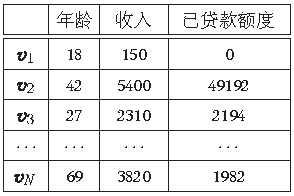
\includegraphics[width=0.45\hsize]{ldp_range_query/figures_others/multi-dimensionalDataset.pdf}
    \vspace{-0.2cm}
    \caption{示例数据集包含 $N$ 个用户以及每个用户的三个属性值:年龄,收入和已贷款额度} 
    \label{Example dataset}
    \vspace{-0.3cm}
\end{figure}

% Assume there are $N$ users, where the $i$-th user has an $m$-dim ordinal record ${\bf{v}}^{m}_i = (v^{(1)}_i, v^{(2)}_i, \cdots, v^{(m)}_i)$, with $v_i^{(j)}$ representing the $j$-th private attribute value owned by user $i$. 
假设参与数据收集的有 $N$ 个用户,其中第 $i$ 个用户拥有一个 $m$ 维数据记录 ${\bf{v}}^{m}_i = (v^{(1)}_i, v^{(2)}_i, \cdots, v^{(m)}_i)$,其中 $v_i^{(j)}$ 表示用户 $i$ 拥有的第 $j$ 维的属性值。
将第 $j$ 个属性值的数据域表示为 $D_j$,
给定一系列范围 $\alpha_j$,$\beta_j$($j=1,2,\cdots,m$),可以计算出一个 $m$ 维范围查询结果。
\begin{equation}
    R_{\bigcap {[\alpha_j,\beta_j]}_{j=1}^{m}}=\frac{1}{N} \sum_{i=1}^{N} \mathbb{I}_{\bigcap{\{\alpha_j \leq v_i^{(j)} \leq \beta_j\}_{j=1}^{m}}}
\end{equation}
其中 $\mathbb{I}_\phi$ 是一个指示函数,如果谓词 $\phi$ 成立则取值为1,否则为0。
% For example, the proportion of people within 20 years to 40 years old constitutes a 1-dim range query, 
% while the ratio of people within 20 years to 40 years old, with salary less than 5000, and with loan amount less than 20000 constitutes a 3-dim range query, 
% where the three dimensions corresponding to age, salary and loan amount, respectively.
\autoref{Example dataset} 给出了一个范围查询的运行示例。
例如,统计年龄在20岁到40岁之间的用户在群体中所占比例是一个一维范围查询,
而统计同时满足年龄在20岁到40岁之间、工资低于5000元和已贷款金额低于20000元的用户在群体中所占比例是一个三维范围查询。

\subsection{分层-间隔优化方法(\myhio)}
\label{exsitingHIO}
基于$B$叉树,\myhio \cite{wang2019answering}将整个数据域分解成互不相交的子集,称为“间隔”。
根节点表示整个数据域,叶节点表示单个值。同一层上的节点表示相同粒度的间隔。然后,\myhio 通过\oue \cite{wang2017locally}算法获得每层节点的频率估计。
当回答范围查询时,\myhio 使用来自不同层的最少间隔完全覆盖查询范围。
例如,当用户的私有属性域大小$|D|=8$,树分支因子$B=2$时,范围查询$[2,7]$可以分解为间隔$[2,3] \cup [4,7]$。
然后,\myhio 将上述两个间隔的估计频率值相加,以回答范围查询。
对于长度为$r$的一般查询,\myhio 最多可以使用$2(B-1)\log_B|D|$个间隔来回答。
与直接使用\fo 机制相比,\myhio 在回答查询时可以有效地减少使用的间隔数量,从而大大减少由于在范围内添加嘈杂的频率值所引起的累积误差。

但是,\myhio 存在两个限制其在实践中适用性的弱点。
1)\myhio 将相同水平的噪声插入到所有间隔的估计频率中。对于间隔较小的节点,扰动噪声往往会掩盖真实频率值,从而降低整个算法的效用。
2)在多维场景中,树层数随维数指数增加。对于高维场景,查询误差随着过多的小值节点而明显地增加。

\subsection{离散哈尔小波变换方法(\mydht)}
\label{exsitingDHT}
\mydht \cite{cormode2019answering} 在域上施加完全二叉树结构,并将用户私有值 $v$ 编码为一组哈尔小波系数。 
\mydht 的动机是,在长度为 $r$ 的范围查询中,相比直接应用\fo ,使用哈尔小波域中估计的值数量更少。

\mydht 也面临一些限制:
1)与 \myhio 相似,\mydht 将相同级别的噪声插入到所有估计的哈尔小波系数中。
对于一些数值较低的系数,噪声倾向于使估计系数偏离实际值,导致查询误差增加;
2)它主要设计用于一维场景,因此在实际应用中存在限制。


\subsection{高维边缘列联表发布方法(\mycalm)}
\label{Consistent Adaptive Local Marginal}
\mycalm \cite{zhang2018calm} 是一种边缘列联表发布 LDP 协议,可在保护隐私的同时构建 $m$ 个属性的联合分布。
\mycalm 不是直接估计包含所有属性边际表,而是根据用户数据域的大小和数据维度的数量进行策略性的属性组合统计,基于属性组合的统计结果可以重建包含所有属性的边际表。
我们注意到,\mycalm 可以用于回答范围查询。
更具体地,为了回答一个多维范围查询,\mycalm 可以将查询包含的重建的边际值求和。

然而,当域大小 $|D|$ 很大时,\mycalm 需要将大量经过扰动的边际值求和以回答范围查询,这可能会向结果中引入过量的噪声。

\subsection{混合维度网格方法(\myHDG)}
\myHDG \cite{yang2020answering}是在LDP场景下回答多维范围查询的现有最好方法。
\myHDG 首先将用户所有属性进行两两组合形成二维数据域,然后基于用户数据域大小将二维数据域精心分桶成粗略的二维网格,并统计每个子数据域内的用户频率。
之后,\myHDG 基于二维范围查询的结果估计出更高维范围查询结果。
为了刻画用户数据的细粒度分布信息,\myHDG 使用粒度更细的一维网格统计每个用户属性的频率分布信息,并结合来自一维和二维网格的信息来回答高维范围查询。

然而,\myHDG 存在下列缺陷:
1) \myHDG 的等粒度网格无法处理各种分布的用户数据。
对于分布较为偏斜的数据集,其用户数据集中在整个数据域的一小部分。因此,在某些网格中噪声误差或非均匀误差会占主导地位,从而降低结果精度;
2) 使用一维网格可能会破坏用户数据中不同属性之间的相关性。

\subsection{总结}
\label{Remarks}

为了克服现有低维机制(\myhio、\mydht)和高维机制(\mycalm、\myHDG)的局限性,我们旨在实现以下两个设计目标:
1)找到合理的区间分解方法,避免引入过多的噪声;
2)设计的机制可以扩展到多维场景,比现有算法具有更好的查询精度。
在这些目标的推动下,我们提出了\myahead,与现有工作存在以下主要差异:
1)与现有方法采用的静态数据编码机制相比,\myahead 采用的是一种自适应、动态的数据编码机制;
2)\myahead 通过合并区间减少噪声对小值节点的影响;
3)所设计的机制可以从一维迁移到多维场景。
接下来,我们将详细阐述\myahead 的动机和设计。

\section{本文方法(\myahead)}
\label{Adaptive Hierarchical Decomposition}

\subsection{设计思路}
\label{Motivation and Overview}
\begin{figure}[!t]
    \centering
    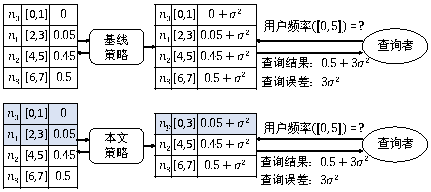
\includegraphics[width=0.75\hsize]{figure/ldp_range_query/figures_others/Motivation3ch.pdf}
    % \vspace{-0.2cm}
    \caption{基线策略与自适应策略}
    \label{Method Motivation}
    % \vspace{-0.3cm}
\end{figure} 

\begin{figure*}[t]
    \centering
    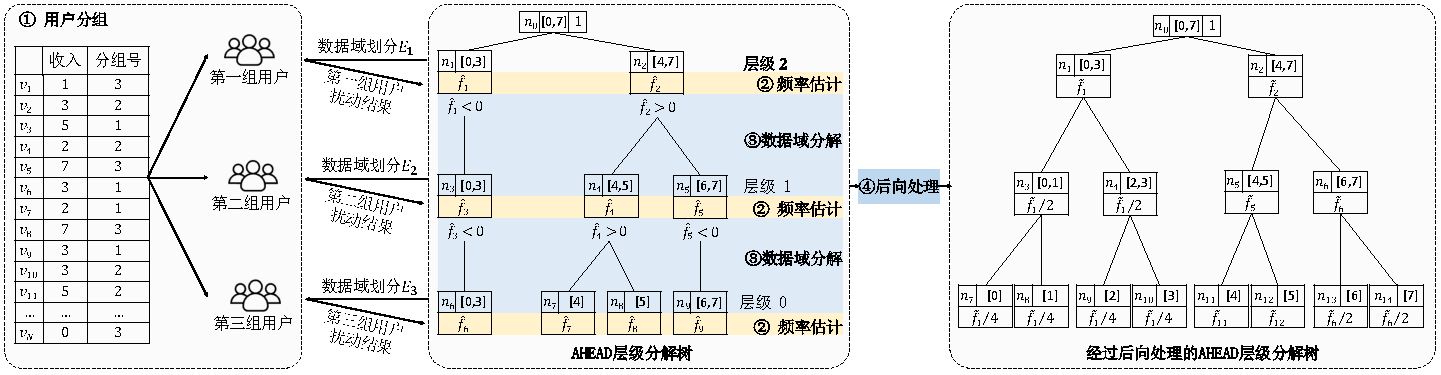
\includegraphics[width=\hsize]{figure/ldp_range_query/figures_others/OverviewAHEAD4ch.pdf}
    % \vspace{-0.4cm}
    \caption{\myahead 的工作流程。从左到右依次展示了\myahead 算法中的四个步骤,即用户分组、频率估计、数据域分解和后向处理。 
    \myahead 根据右侧子图中的树回答范围查询。} 
    \label{AHEAD method}   
    % \vspace{-0.4cm}
\end{figure*}

在这个章节中,我们使用一个例子来说明现有算法的局限性以及\myahead 的合理性。
如\autoref{Method Motivation}所示,左侧的表格显示了带有相应实际频率值的数据区间。
例如,区间$[0,1]$的真实频率值为$0$,意味着这个区间内没有用户数据。
然后,中间的表格显示了使用不同策略分别估计的区间频率值。
其中,$\sigma^2$代表扰动过程中引入的噪声方差。
右侧的剩余部分展示了基于估计值回答查询的过程。

首先,我们关注基线策略,例如\myhio。
基线策略选择发布每个区间的估计频率值。
每个估计值通过\fo 机制引入了“噪声误差”,以满足LDP的要求。
对于区间$[0,1]$,它的真实值为$0$,这意味着这些区间的估计值完全被噪声填充。
当回答范围查询时,例如区间$[0,5]$的用户频率,提问者想知道区间$[0,5]$的频率值。
基线策略的结果是$0.5 + 3\sigma^2$。
在这个例子中,区间$[0,1]$的真实值并未对查询答案做出贡献,却带来了同等程度的噪声,降低了基线策略的查询准确度。

另一方面,对于自适应策略,如果我们知道各区间的真实频率值,就可以合并区间$n_0$和$n_1$,只需要估计合并后的区间$n_p$。
当需要输出区间$[0,5]$的用户频率时,自适应策略的结果是$0.5 + 2\sigma^2$,与基线方法相比,将噪声误差降低了30\%。

自适应策略可以有效减小扰动噪声对频率值较小区间的影响。
但是,当查询需要使用合并区间的部分区域时,自适应策略必须通过对合并区间内频率分布的作出假设才能进行后续的计算。
主流方法是假设合并区间内的频率分布满足均匀分布\cite{ioannidis2003history},即合并区间用户频率均匀分布。
如果实际用户频率不满足该假设时,自适应策略的结果将会产生“非均匀误差”。
例如,如果查询者想要知道区间$[2,3]$的用户频率,那么自适应策略将基于两个区间的尺寸在均匀分布的假设下进行计算,即 $[0,3]$ 区间频率值的一半。
与基准策略相比,自适应策略将噪声误差从 $\sigma^2$ 降低到 $\frac{\sigma^2}{2}$,
同时它也带来了非均匀误差 $0.05 - \frac{0.05}{2} = 0.025$。

自适应性通过合并区间来减少噪声误差,同时通过假设均匀分布引入了非均匀误差。
因此,我们希望找到最优的数据域分解来平衡这两种误差,进而减少总查询误差。
文献\cite{muthukrishnan1999rectangular}指出即便是在二维数据场景下,找到最优的数据域分解是困难的,那么在隐私约束下这个问题将变得更具挑战性。 
综上,我们提出了一种基于自适应层级递归划分策略(详见\autoref{Workflow of ahead}),旨在平衡噪声误差和非均匀误差,并解决现有方法的不足。

\subsection{一维数据场景\myahead 的工作流程}
\label{Workflow of ahead}
在本章,我们通过\autoref{AHEAD method}中的例子阐述\myahead 的工作流程。
聚合器希望基于\myahead 完成有关用户收入的范围查询任务。
收入数据被分成了8个有序级别,即域大小$|D|=8$。
树的扇出度$B=2$,这意味着\myahead 树的每个节点最多有两个子节点。
在\myahead 原型树的每个节点中,$n_i$表示节点索引,$[a,b]$表示节点的区间,$\hat{f_i}$表示估计的频率值。
值得注意的是,\myahead 采用了抽样原则\cite{cormode2019answering},将全部参与用户划分为子用户组,每组用户使用全部隐私预算。
抽样原则可以显著减少本地差分隐私场景中查询结果的噪声误差\cite{nguyen2016collecting, wang2017locally, wang2019locally}
% (有关更多详细信息,请参见\autoref{The rationality of sampling principle})。
接下来,我们将\myahead 的工作流程分为四个步骤。

\mypara{第一步:用户分组}

如\autoref{AHEAD method}中所示的左虚线框中,
聚合器确定分区数$c$,其中$c=\log_B|D|$旨在确保将用户分配到\myahead 树的每一层。
用户随机选择在范围$[1,2,3,\cdots,c]$内的组号。
此外,用户还可以利用他们的公共信息来选择组,例如帐户注册时间,用户ID等。
分区过程应确保每个组代表整体人口,具有相似数量的用户。

\mypara{第二步:频率估计}

在中间的虚线框中,聚合器首先建立代表整个数据域的根节点$n_0$。
然后,聚合器对域进行初始分解,即将整个域分成$B$个相等大小的区间,然后将区间节点连接到根节点$n_0$上。
根节点的子节点代表一种将整个数据域分割的方法,表示为数据域分解$E_1$。
聚合器选择第一组用户,并向他们发送分解$E_1$和隐私预算$\epsilon$。
第一组用户中的每个用户将自己的私有值$v$投影到$E_1$的区间上,并通过\oue 上传$v$的投影值。在接收到用户报告后,聚合器使用聚合算法获得估计的频率分布$\hat{F_1}$,表示落在每个节点区间内的用户比例。

\mypara{第三步:数据域分解}

聚合器将$\hat{F_1}=\{\hat{f_1}, \hat{f_2}\}$的每个频率值与阈值$\theta$进行比较,并决定是否进一步分割$E_1=\{[0,3], [4,7]\}$中的相应区间。
具体来说,由于$\hat{f_2}$大于设定的$\theta$,因此应将$E_1$中的相应区间$[4,7]$分成$B$个大小相等的子区间$[4,5]$和$[6,7]$。
而节点$n_1$的频率值$\hat{f_1}$小于$\theta$,那么区间$[0,3]$不需要进一步划分。
对于新的区间节点,我们将它们附加到相应的父区间节点上。
当$\hat{F_1}$中的所有元素都被遍历时,我们可以获得一组新的数据域分解$E_{2}$。

然后,聚合器将分解$E_{2}$发送给第二组用户并获得估计的频率分布$F_2$。聚合器重复以上步骤,直到应用所有用户组并获得\autoref{AHEAD method}中显示的\myahead 原型树。由于估计频率小于阈值$\theta$,\myahead 不会在后续交互中分解区间$[0,3]$和$[6,7]$。
为了满足LDP要求,区间$[0,3]$和$[6,7]$依然参与后续用户组的频率估计。

在构建原型树时,\myahead 分别估计每个层的频率分布。
在这个过程中,\myahead 没有考虑树中频率值的约束,例如子节点的频率值之和等于其父节点。
因此,在步骤四中,我们通过对节点估计进行“非负性”和“加权平均”处理,来进一步提高\myahead 查询结果的准确性。

\mypara{第四步:后向处理}

% 后向处理包含两个步骤:非负性和加权平均。
首先是对节点频率值进行非负性处理,\myahead 使用Norm-Sub \cite{wang2019consistent}对同一层中的节点进行处理,以确保节点的估计频率为非负数且频率总和为1。
\myahead 将负值转换为0,并计算正值的总和与1之间的差异。
接下来,每个正值减去平均差异,该平均差异是通过将总差异除以正估计值的数量获得的。
非负性处理过程重复进行,直到所有节点的频率值都变为非负数。

然后\myahead 从下往上对所有节点的频率值进行加权平均。
\myahead 计算非叶节点$n$和其子节点频率值的加权平均值,以更新$n$的估计频率,即通过融合$n$的多个估计结果来降低扰动噪声的影响。

\begin{equation}
    \label{weighted average}
    \tilde{f}(n)=\left\{
    \begin{array}{rcl}
    \lambda_1\hat{f}(n) + \lambda_2 \sum_{u \in child(n)}\hat{f}(u), &   \mbox{如果$u$是一个叶子节点} \\
    \lambda_1\hat{f}(n) + \lambda_2 \sum_{u \in child(n)}\tilde{f}(u),    & \mbox{其他情况}  \\
    \end{array}\right.
\end{equation}

权重 $\lambda_1$ 和 $\lambda_2$ 与估计值的方差成反比,即 $\lambda_1 = \frac{\myvar_{child(n)}}{\myvar_{child(n)} + \myvar_{(n)}}$ 和 $\lambda_2 = \frac{\myvar_{(n)}}{\myvar_{child(n)} + \myvar_{(n)}}$,其中 $\myvar_{child(n)}$ 表示节点 $n$ 的子节点方差之和,$\myvar_{n}$ 表示节点 $n$ 的方差。
$\tilde{f}$ 表示 $\hat{f}$ 的后向处理版本,将用于回答查询。
% 加权平均过程可以最小化噪声的幅度,如下定理所示。 \autoref{theorem: weighted average} 的证明可以在 \autoref{The proof of weighted average} 中找到。

\begin{theorem}
    \label{theorem: weighted average}
    使用{\rm\autoref{weighted average}}来更新节点的频率,节点$n$可以达到最小扰动方差。
\end{theorem} 
\begin{proof}
    根据文献{\rm\parencite{wanglocally}},经过扰动后的区间估计频率值$\hat{f}$近似于$f+X$,其中$f$是真实的频率值,$X$是一个服从\Gaussian 分布$\mathcal{N}(0,\myvar_{\oue})$的随机变量。
    假设$u$为叶子节点,那么有
    \begin{align}
    \hat{f}(n) = f(n) + \mathcal{N}(0,\myvar_{(n)}) \nonumber
    \end{align}
    \begin{align}
    \sum_{u \in child(n)} \hat{f}(u) = \sum_{u \in child(n)}f(u) + \mathcal{N}(0,\myvar_{(u)}) \nonumber
    \end{align}
    节点$n$的区间等于其子节点区间的组合。因此
    \begin{align}
    f(n) = \sum_{u \in child(n)}f(u) \nonumber
    \end{align}
    设加权平均的系数为$\lambda_1$和$\lambda_2$,$f(n)$和$\sum_{u \in child(n)}f(u)$之间的加权平均值是节点$n$频率的无偏估计,其中$\lambda_1+\lambda_2=1$。
    \begin{align}
    \tilde{f}(n)=\lambda_1\hat{f}(n)+\lambda_2\sum_{u \in child(n)}\hat{f}(u) \nonumber
    \end{align}
    $\tilde{f}(n)$的方差等于$\lambda_1^2\myvar_{(n)}+\lambda_2^2\myvar_{child(n)}$。
    当且仅当
    \begin{align}
    \lambda_1=\frac{\myvar_{child(n)}}{\myvar_{child(n)}+\myvar_{(n)}} \nonumber,~~~~
    \lambda_2=\frac{\myvar_{(n)}}{\myvar_{child(n)}+\myvar_{(n)}},\nonumber
    \end{align}
    我们可以最小化$\tilde{f}(n)$的方差。
    加权平均后,扰动噪声仍服从\Gaussian 分布。
    因此,当$u$不是叶子节点时,上述证明仍然成立。
\end{proof}

最后,从根节点到叶子节点,\myahead 基于均匀分布假设递归地分解父节点的频率值,并获取完整的层级分解树以回答范围查询,具体如\autoref{AHEAD method} 的最右边子图所示。

\subsection{高维数据场景\myahead 的工作流程}
\label{Extension to Multi-dimensional Settings}
\subsubsection{二维数据场景}
首先我们讨论二维数据场景。
我们假设所有属性都具有相同的域 $D = \{1, 2, \cdots, d\}$,
其中 $d$ 是树扇出度 $B$ 的幂。
如果实际用户的数据域不同,我们可以添加一些填充值使所有数据域长度一致。
一维数据场景和二维数据场景的主要区别在于分解过程,体现在\autoref{Construct 1-dim prototype tree} 的第4行和第9行。
对于一维数据场景,\myahead 按层次划分整个数据域 $[1, |D|]$。
整个数据域划分为粒度不同的子区间。
对于二维数据场景,整个数据域变成了一个正方形区域 $[1, |D|] \times [1, |D|]$。
所以,\myahead 需要生成不同粒度的二维网格来分解整个数据域。
我们在\autoref{Multi-dimensional tree}给出了二维数据场景的\myahead 的工作流程,并在\autoref{Construct 2-dim prototype tree} 提供了相应的伪代码。
在上述示例中,用户私有属性的数据域大小为 $8\times8$,树扇出度 $B=4$。
与一维数据场景类似,二维\myahead 也需要四个步骤来估计用户的频率分布。

\mypara{用户分组}
用户在 $\{1, 2, 3, \cdots, c\}$ 的集合中随机选择用户组编号,其中 $c = \log_B|D|^2$。

\mypara{频率估计}
接着,聚合器将整个数据域划分为 $B$ 个等大小的正方形区域,并将初始数据划分发送给第一组用户。
用户将其私有数据投影到初始划分中,并通过 \oue 上传其数据。
服务器使用聚合算法获取估计的频率分布,该分布表示落入每个子域内的用户比例。

\mypara{数据域分解}
然后,聚合器将每个估计频率值与阈值 $\theta$ 进行比较,决定是否进一步划分相应的子域。
重复频率估计和数据域分解过程,\myahead 递归地分解域并构建 \myahead 原型树。

\mypara{后向处理}
最后,\myahead 在每个层内执行非负性处理,并在两个相邻层之间执行父节点和子节点估计频率之间的加权平均,以进一步减小估计误差。
基于均匀分布假设,\myahead 得到完整的树结构来回答范围查询。

因为查询结果的误差随使用节点数量的增加而增加,为了减少查询误差,\myahead 更倾向于使用粗粒度节点来回答查询。
如\autoref{Multi-dimensional tree} 所示,\myahead 回答一个二维查询 $[0,5]\times[0,5]$。 
\myahead 从树的顶层向下搜索,并计算范围查询完全覆盖的子域的频率之和。
范围查询完全覆盖了顶层 $[0,3]\times[0,3]$ 的区域以及中间层的五个区域 $[0,1]\times[4,5]$、$[2,3]\times[4,5]$、$[4,5]\times[4,5]$、$[4,5]\times[0,1]$、$[4,5]\times[2,3]$(这些区域用蓝色突出显示),
因此查询答案为 $(\tilde{f}1 + \tilde{f}9 + \tilde{f}{11} + \tilde{f}{13} + \tilde{f}{14} + \tilde{f}{4}/4)$。

对于二维范围查询,我们设置$B=2^2$,即每个维度的树扇出度为$2$。
作为比较,我们在实验中还给出了$B=4^2$的结果。
由于$\theta$的推导不涉及维度变化,
因此我们仍然根据\autoref{theta setting1}选择$\theta$。

\subsubsection{三维及以上数据场景}

\myahead 可以通过两种方式扩展到更高维度。

\mypara{直接估计算法(Direct Estimation,\de)}
基于扇出度为 $B=2^m$ 的树,\myahead 同时分解 $m$ 个维度。
例如,\myahead 将三维域视为一个立方体,然后聚合不同粒度的子立方体的频率以回答查询。
在 \autoref{theta setting1} 的阈值设置下,\myahead 可以很好地控制子域的整体估计误差。
然而,叶节点数目随着维度呈指数级增长,这使得在高维数据集上查询答案过程非常耗时。

\mypara{利用低维估计算法(Leveraging Low-dimensional Estimation,\lle)}
为了解决数据维度上升引起的子域爆炸问题,
\lle 首先将属性两两配对,然后为每个属性对构建一个二维\myahead 树。
接着,在回答一个 $m$ 维查询时,\lle 构建一个包含 $2^m$ 个关联查询的查询集合。
最后,利用二维频率作为约束条件,\lle 通过最大熵优化估计所有 $2^m$ 个查询的频率值。
接下来,我们将详细介绍\lle 方法的三个步骤。
\begin{enumerate}
\item [1)] \mypara{构建二维树} \myahead 将所有属性成对分组,形成 $C_m^2$ 个二维属性对。
然后,\myahead 分别为这 $C_m^2$ 个二维属性对进行二维频率分布估计,即总共构建了 $C_m^2$ 个二维树。
\item [2)] \mypara{属性分布对齐} 
\myahead 需要在二维树集合中进行 $m$ 个数据维度的边际分布的对齐。
这保证了从不同二维树中进行某一属性的范围查询时结果的唯一性。
例如,属性 $a$ 参与了 $(m-1)$ 个属性对。
假设这 $(m-1)$ 个二维树分别为 $\{T_1, T_2, T_3, \cdots, T_{m-1}\}$,每个树除了根节点外都有 $\ell$ 层。
对于整数 $k \in [1, B^{\ell/2}]$,我们定义 $f_{T_i}(a, \ell, k)$ 为属于第 $\ell$ 层的 $T_i$ 节点的频率之和,
这些节点所对应的子域在属性 $a$ 上的覆盖范围为 $[(k-1)\cdot\frac{|D|}{B^{\ell/2}}+1, k\cdot\frac{|D|}{B^{\ell/2}}]$。
为了使所有 $f_{T_i}(a, \ell, k)$ 的频率分布在属性$a$的边际分布上保持一致,
\myahead 计算它们的加权平均值 $f(a, \ell, k) = \sum_{i=1}^{m-1}\lambda_{i} \cdot f_{T_i}(a, \ell, k)$,
其中 $\lambda_i$ 是 $f_{T_i}(a, \ell, k)$ 的权重,且 $\sum_{i=1}^{m-1}\lambda_i = 1$。
设置的权重值 $\lambda$ 用来最小化 $f(a, \ell, k)$ 的方差,
即 $\myvar[f(a, \ell, k)] = \sum_{i=1}^{m-1}\lambda_i^2\cdot \myvar[f_{T_i}(a, \ell, k)]$,其中 $\myvar[f_{T_i}(a, \ell, k)]$ 是用于计算 $f_{T_i}(a, \ell, k)$ 的节点理论方差之和。
当权重与估计值的方差成反比时,$\myvar[f(a, \ell, k)]$ 最小\cite{yang2020answering}。
因此,最优权重 $\lambda_i = \frac{1}{\myvar[f_{T_i}(a, \ell, k)]}/\sum_{i=1}^{m-1}\frac{1}{\myvar[f_{T_i}(a, \ell, k)]}$。
我们通过在原始估计频率上添加 $(f(a, \ell, k) - f_{T_i}(a, \ell, k))/B^{\ell/2}$ 来更新 $T_i$ 中原有的频率估计值,最终使每个 $f_{T_i}(a, \ell, k)$ 等于 $f(a, \ell, k)$。
根据文献{\rm\parencite{qardaji2014priview}} 的分析结论,
关于属性 $a$ 在 $\{T_1, T_2, T_3, \cdots, T_{m-1}\}$ 进行属性分布对齐不会影响其他属性的频率分布。
% ${T_1, T_2, T_3, \cdots, T_{m-1}}$ 在不改变的情况下达成对 的一致。
因此,我们可以按任意属性顺序进行属性分布对齐,\myahead 可以实现所有 $m$ 个属性的一致性。注意到每个二维树有 $\ell$ 层,\myahead 需要对所有 $\ell$ 层分别执行属性分布对齐。
\item [3)] \mypara{最大熵优化} 
我们采用了最大熵原理\cite{qardaji2014priview},基于二维查询的结果估计 $m$ 维查询结果。
具体来说,对于一个 $m$ 维范围查询 $q$,我们可以定义一组范围查询:
$$Q(q)=\left\{\wedge\left(a_{j},\left[\alpha_{j}, \beta_{j}\right] \text { or }\overline{\left[\alpha_{j}, \beta_{j}\right]}\right) \mid a_{j} \in A\right\}\text{,}$$
其中 $[\alpha_t, \beta_t]$ 表示查询区间,$\overline{\left[\alpha_{t}, \beta_{t}\right]}$ 是其补集。
对于 $2^m$ 个查询 $g \in Q(q)$,
我们定义 $f_q(g)$ 为 $Q(q)$ 查询结果集合。
我们可以获得 $Q(q)$ 对应的二维查询集合以及其对应的查询结果集合$f_{q^{(j,k)}}$:
$$Q(q^{(j,k)})=\left\{\left(a_{j},\left[\alpha_{j}, \beta_{j}\right] \text { or }\overline{\left[\alpha_{j}, \beta_{j}\right]}\right) \wedge \left(a_{k},\left[\alpha_{k}, \beta_{k}\right] \text { or }\overline{\left[\alpha_{k}, \beta_{k}\right]}\right)\right\}\text{,}$$
对于任何查询 $g^{(j,k)} \in Q(q^{(j,k)})$,我们使用 $f_{q^{(j,k)}}(g^{(j,k)})$ 来表示其查询结果。
例如,对于一个 $g^{(j,k)} \in Q(q^{(j,k)})$,$f_{q}(g^{(j,k)})$ 表示通过对 $Q(q)$ 集合中的查询结果求和,以构建高维查询 $g^{(j,k)}$ 的结果 $f_q$。
接着,我们可以通过求解下列优化问题得到具体的高维查询结果。
$$
\begin{array}{ll}
\text { maximize } & -\sum_{g \in Q(q)} f_{q}(g) \cdot \log \left(f_{q}(g)\right) \\
\text { subject to } & \forall_{g \in Q(q)} f_{q}(g) \geq 0 \\
& \forall_{a_j, a_k \in A} \forall_{g^{(j, k)} \in Q\left(q^{(j, k)}\right)} f_{q^{(j, k)}}(g^{(j, k)})=f_{q}(g^{(j, k)})
\end{array}
$$
以上优化问题可以通过现有凸优化工具来解决。
为了更快速的计算出查询结果,降低查询延迟,\myahead 采用文献{\rm\parencite{yang2020answering}}提出的加权更新算法,
该算法在降低计算复杂度的同时实现了与最大熵估计相当的精度。
\end{enumerate}

\de 方法的实现相对简单,而且用户分区的数量不会随着维数的增加而增加。然而,\de 中的 \myahead 树在高维情况下可能非常大,从而使得树的构建和查询回答过程变得耗时。
相比之下,\lle 方法将属性成对组合,为每个属性对构建一个二维 \myahead 树,使得每棵树的规模不会太大。
% 我们在 \autoref{Effectiveness of ahead for high-dimensional Range Query} 中从经验上展示了这两种策略的性能,并讨论了如何在它们之间进行选择。
% 之前的方法也利用最大熵优化将低维机制有效地扩展到高维场景中。例如,\PriView\cite{qardaji2014priview} 提出构建低维视图,即二维、三维边缘表,并将最大熵优化应用于从视图中重建更高维的边缘表。
\begin{algorithm}[!h]
    \caption{构建二维\myahead 层级分解树}
    \label{Construct 2-dim prototype tree}
	\begin{algorithmic}[1]
        % \REQUIRE All users’ value set $V = \{v_1, v_2,\ldots,v_N \}$, attribute domain $D$, tree fanout $B$, privacy budget $\epsilon$, threshold $\theta$
        % \ENSURE \myahead Tree $T$
        \REQUIRE 用户私有值 $V=\{v_1, \ldots, v_N\}$,数据域 $D$,树扇出度 $B$,隐私预算 $\epsilon$,阈值 $\theta$。
        \ENSURE 经过后向处理的\myahead 层级分解树 $T$
		\STATE $c = {\log_B}|D|^2$
        \STATE $//$ 用户划分
        % \STATE Randomly divide users into $c$ parts $\left\{ V_1, V_2, \ldots, V_c \right\}$
        % \STATE Create the root node of tree $T$ with initial interval $e^0_0 = [1, |D|] \times [1, |D|]$ and $\operatorname{T.node}(e^0_0).frequency = 1$ 
        \STATE 随机将所有用户划分为 $c$ 个用户组 $\left\{ V_1, V_2, \ldots, V_c \right\}$
        \STATE 创建表示整个二维数据域的树 $T$的根节点 $e^0_0 = [1, |D|] \times [1, |D|]$ 和 $\operatorname{T.node}(e^0_0).\operatorname{frequency = 1}$
		\FOR {$i$ from 1 to $c$}
            \STATE $//$ 数据域分解
            \FOR {$j$, node in enumerate($T.\operatorname{node}(\operatorname{level}=i-1)$)}
            \IF {$\operatorname{node.frequency} > \theta$}
            % \STATE Divide $\operatorname{interval} e^{i-1}_j$ into $B$ disjoint intervals $\{e^{i-1}_{j,k}\}$
            \STATE 将二维区间 $e^{i-1}_j$ 分解为 $B$ 个不相交的二维子区间 $\{e^{i-1}_{j,k}\}$
            \FOR {$k$ from $1$ to $B$}
    		\STATE $\operatorname{node.add\_child}(e^{i-1}_{j,k})$
            \ENDFOR
            \ELSE
            \STATE $\operatorname{node.add\_child}(e^{i-1}_{j})$
            \ENDIF 		
            \ENDFOR

            \STATE $//$ 频率估计
            \STATE $F = \fo(V_i, T.\operatorname{node}(\operatorname{level}=i).\operatorname{interval}, \epsilon)$
            \FOR {$k$, node in enumerate $T.\operatorname{node}(\operatorname{level}=i)$}
    		\STATE $\operatorname{node}.\operatorname{frequency} = F[k]$
            \ENDFOR
        \ENDFOR
        \STATE $//$ 后向处理
        \STATE 运行 \autoref{alg:1-dim post_processing}
        \STATE 返回 $T$
	\end{algorithmic}
\end{algorithm}

% \begin{algorithm}[!h]
% 	\caption{Post-processing}
% 	\label{alg:2-dim post_processing}
% 	\begin{algorithmic}[1]
%         \REQUIRE \myahead tree $T$, tree fanout $B$
%         \ENSURE \myahead tree $T$
%         \FOR {$i$ from $1$ to $c$}
% 		\STATE norm\_sub($T.\operatorname{node(level=i)}.\operatorname{frequency}$)
%         \ENDFOR    
%         \FOR {$j$ from $c-1$ to $1$}
%             \FOR {\_, node in enumerate $T.\operatorname{node}(level=j)$}
%             \STATE $f_1$ = node.frequency, $f_2$ = $\sum{\operatorname{node.children().frequency}}$
% 		    \STATE node.frequency = $\lambda_1$$f_1$ + $\lambda_2$$f_2$
%             \ENDFOR 
%         \ENDFOR    
%         \FOR {$k$ from $1$ to $c$}
%             \FOR {\_, node in enumerate $T.\operatorname{node}(level=k)$}
%                     \IF {node.children() == None}
% 		            \STATE $\operatorname{node}.\operatorname{add\_children}()$
% 		            \STATE $\operatorname{node}.\operatorname{children()}.\operatorname{frequency} = \operatorname{node}.\operatorname{frequency}/B$
%                     \ENDIF
%             \ENDFOR 
%         \ENDFOR    
        
%     \end{algorithmic}
% \end{algorithm}

\begin{figure*}[t]
    \centering
    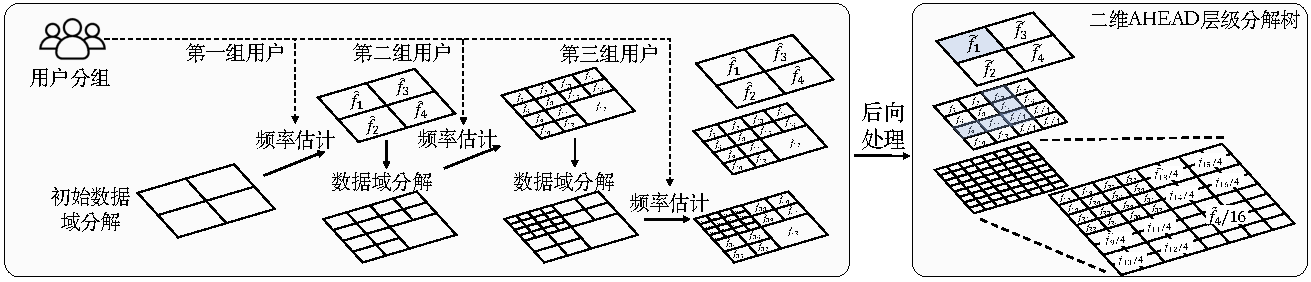
\includegraphics[width=\hsize]{figure/ldp_range_query/figures_others/GridAHEAD_workflow2ch.pdf.pdf}
    \vspace{-0.7cm}
    \caption{
        % 2-dim \myahead algorithm, 
    % where the decomposition is implemented by decomposing both dimensions simultaneously.
    \myahead 构建二维层级分解树的流程。在数据域分解过程中,\myahead 同时对二维数据域的两个维度同时进行分解。}
    \vspace{-0.4cm}
    \label{Multi-dimensional tree}
\end{figure*}

\subsection{算法本地差分隐私合规性及误差分析}
\label{Privacy and Utility Analysis}

\subsubsection{本地差分隐私合规性}

\myahead 与所有用户顺序交互 \cite{joseph2019role, joseph2020exponential, duchi2013local, acharya2020interactive, kasiviswanathan2011can}。
在整个数据收集过程中,每个用户只通信一次(\autoref{Workflow of ahead} 中的第2步),
但随机化取决于之前用户的消息(\autoref{Workflow of ahead} 中的第3步)。
每个用户的私有数据通过保隐私的 \oue 协议传输到聚合器,不泄露其他用户的任何信息。

\begin{theorem}
    \label{satisfy LDP}
    \myahead 满足 $\epsilon$-LDP.
\end{theorem} 
\begin{proof}
    在第一步中,用户在 $[1,2, \cdots, c]$ 中随机选择他们的组ID,不需要使用隐私预算。
    在第二步和第三步中,\myahead 逐个与用户交互,每个用户产生一个输出。
    在第四步中,\myahead 不会触及用户的私人数据,因此不会产生额外的隐私预算消耗。
    因此,如果聚合器与用户的交互过程(第二步和第三步)符合 $\epsilon$-LDP,则 \myahead 满足 $\epsilon$-LDP \cite{joseph2020exponential}。
    
    在与用户的交互过程中,\myahead 使用隐私预算 $\epsilon$ 并基于 \oue 协议进行频率估计。
    对于任意的两个用户私有数据值 $v_1, v_2 \in D$,上传结果都是经过 \oue 扰动的带噪声的二进制向量 $O$。
    我们选取第$g$组用户为分析对象,其他组同理可证。
    \begin{align}\label{6}
        \frac{\Pr{O|v_1, g}}{\Pr{O|v_2, g}} &= \frac{\Pi_{i=1}^{\ell}\Pr{O[i]|v_1, g}}{\Pi_{i=1}^{\ell}\Pr{O[i]|v_2, g}} \nonumber \\
                              &= \frac{\Pi_{i=1}^{\ell}\Pr{O[i]|v_1} \cdot \Pr g}{\Pi_{i=1}^{\ell}\Pr{O[i]|v_2} \cdot \Pr g} \nonumber \\
                                                &\leq{\frac{\Pr{O[v_1]=1|v_1}\Pr{O[v_2]=0|v_1}}{\Pr{O[v_1]=1|v_2}\Pr{O[v_2]=0|v_2}}} \nonumber \\
                                                &= \frac{p}{q}\cdot\frac{1-q}{1-p} \nonumber \\
                                                &= \frac{1/2}{1/(1+e^\epsilon)}\cdot\frac{1-1/(1+e^\epsilon)}{1-1/2}= e^\epsilon, 
    \end{align}

    其中,$\ell$是$O$的长度。
    $p$和$q$是\oue 协议的翻转概率。
    当$p = \frac{1}{2}$,$q = \frac{1}{(e^\epsilon +1)}$时,\oue 可以获得最小方差 {\rm\cite{wang2017locally}}。
    从{\rm\autoref{6}},第二步满足$\epsilon$-LDP。
    因为第三步处理对象是扰动后的数据,即未接触用户的原始私有数据,因此没有消耗额外的隐私预算。
    综上,\myahead 算法满足$\epsilon$-LDP。
\end{proof}


\subsubsection{查询结果误差分析}
真实查询结果和\myahead 输出结果之间的误差来源于三个方面。
其中,扰动噪声误差和采样误差源于 \oue 的扰动和用户采样过程,
非均匀误差是由于在 \myahead 树中,一些区间的频率值是由较大区间的值近似计算而来的。

\mypara{噪声误差和采样误差} 
如\autoref{myoue}所示,尽管 \oue 可以获得频率值的无偏估计,但仍存在由扰动引起的估计方差。
此外,\myahead 将用户分为 $c$ 组,并使用每个用户组来表示所有用户的频率估计。 
基于 \cite{yang2020answering} 中的分析,采样误差是一个常数,远小于插入的噪声。
由于每个用户随机选择其中一个 $c$ 组来报告私有数据,每个组的用户数量近似于 $\frac{N}{c}$。
根据\autoref{OUEVAR},扰动噪声 $X$ 的方差与组数 $c$ 成比例,即 $\sigma^2 = c \cdot \frac{4e^{\epsilon}}{N\left(e^{\epsilon}-1\right)^{2}}$。
由于阈值设置的原因,一些细粒度区间的频率值可能无法直接估算。
对于未估算的间隔,其频率值应该从更大的间隔中计算,即 \myahead 树中的父节点。
如果未估算的间隔的频率值是从一个比它大小大 $k$ 倍的大区间中计算的,则 \myahead 将大区间的估计频率的 $\frac{1}{k}$ 分配给未估算的区间。
因此,未估算区间的噪声误差可以视为来源于随机变量 $\frac{X}{k}$。

\mypara{非均匀误差}
对于一个没有直接估计的区间 $n$,假设其真实频率值为 $f_n$。
其对应的父节点区间的尺寸为 $n$ 的 $k$ 倍,此处 $k$ 的含义与噪声误差和采样误差部分中的 $k$ 相同。
假设父节点区间的频率分布满足均匀分布\cite{qardaji2013differentially}。
那么,区间 $n$ 的分配频率值为 $\frac{f_p}{k}$,其中 $f_p$ 是父节点区间的真实频率值。
如果区间 $p$ 中的值满足均匀分布时,则没有非均匀误差,即 $f_n = \frac{f_p}{k}$。
如果区间 $p$ 中的值不符合均匀分布时,区间 $n$ 的频率值偏差为 $|f_n - \frac{f_p}{k}|$。
因此,非均匀误差受父节点区间 $p$ 真实分布的影响。
如果频率分布接近均匀分布,则非均匀误差较小。
否则,非均匀误差将变大,并且非均匀误差的上限取决于真实频率值 $f_p$,即 $|f_p - \frac{f_p}{k}|$。
综上,在节点真实频率更均匀分布的情况下,\myahead 的表现更好,因为非均匀误差更小。

\begin{algorithm}[!t]
	\begin{algorithmic}[1]
        \REQUIRE 用户私有值 $V=\{v_1, \ldots, v_N\}$,数据域 $D$,树扇出度 $B$,隐私预算 $\epsilon$,阈值 $\theta$。
        \ENSURE 经过后向处理的\myahead 层级分解树 $T$
		\STATE $c = {\log_B}|D|$
		\STATE $//$ 用户划分
        \STATE 随机将所有用户划分为 $c$ 个用户组 $\left\{ V_1, V_2, \ldots, V_c \right\}$
        \STATE 创建表示整个数据域的树 $T$的根节点 $e^0_0 = [1, |D|]$,并初始化其频率值$T.\operatorname{node}(e^0_0).\operatorname{frequency} = 1$
		\FOR {$i$ from 1 to $c$}
            \STATE $//$ 数据域分解
            \FOR {$j$, node in enumerate($T.\operatorname{node}(\operatorname{level}=i-1)$)}
            \IF {$\operatorname{node.frequency} > \theta$}
            \STATE 将区间 $e^{i-1}_j$ 分解为 $B$ 个不相交的子区间 $\{e^{i-1}_{j,k}\}$
            \FOR {$k$ from $1$ to $B$}
    		\STATE $\operatorname{node.add\_child}(e^{i-1}_{j,k})$
            \ENDFOR
            \ELSE
            \STATE $\operatorname{node.add\_child}(e^{i-1}_{j})$
            \ENDIF    		
            \ENDFOR
            \STATE $//$ 频率估计
            \STATE $F = \fo(V_i, T.\operatorname{node}(\operatorname{level}=i).\operatorname{interval}, \epsilon)$
            \FOR {$k$, node in enumerate $T.\operatorname{node}(level=i)$}
    		\STATE $\operatorname{node}.\operatorname{frequency} = F[k]$
            \ENDFOR
        \ENDFOR
        \STATE $//$ 后向处理
        \STATE 运行 \autoref{alg:1-dim post_processing}
        \STATE 返回 $T$
	\end{algorithmic}
    \caption{构建一维\myahead 层级分解树}
    \label{Construct 1-dim prototype tree}
\end{algorithm}

\begin{algorithm}[!t]
	\caption{后向处理}
	\label{alg:1-dim post_processing}
	\begin{algorithmic}[1]
        \REQUIRE \myahead 层级分解树 $T$, 树扇出度 $B$
        \ENSURE 经过后向处理的\myahead 层级分解树 $T$
        \FOR {$i$ from $1$ to $c$}
		\STATE norm\_sub($T.\operatorname{node}(\operatorname{level}=i).\operatorname{frequency}$)
        \ENDFOR    
        \FOR {$j$ from $c-1$ to $1$}
            \FOR {\_, node in enumerate $T.\operatorname{node}(\operatorname{level}=j)$}
            \STATE $f_1$ = $\operatorname{node}.\operatorname{frequency}$, $f_2$ = $\sum{\operatorname{node.children().frequency}}$
		    \STATE $\operatorname{node}.\operatorname{frequency}$ = $\lambda_1$$f_1$ + $\lambda_2$$f_2$
            \ENDFOR 
        \ENDFOR    
        \FOR {$k$ from $1$ to $c$}
            \FOR {\_, node in enumerate $T.\operatorname{node}(\operatorname{level}=k)$}
                    \IF {$\operatorname{node}.\operatorname{children()}$ == None}
		            \STATE $\operatorname{node}.\operatorname{add\_children}()$
		            \STATE $\operatorname{node}.\operatorname{children()}.\operatorname{frequency} = \operatorname{node}.\operatorname{frequency}/B$
                    \ENDIF
            \ENDFOR 
        \ENDFOR    
    \end{algorithmic}
\end{algorithm}

\subsection{算法参数 $\theta$ 和 $B$ 设置分析}
\label{Selection parameters}
\myahead 的最重要的参数是分解阈值$\theta$和树的扇出度$B$。
基于\autoref{satisfy LDP},\myahead 已满足LDP的要求。
在本节中,我们的目标是分析如何设置算法参数$B$和$\theta$,以最大化\myahead 的查询结果的精度。
在实际中,参与数据收集的用户数量较大。所以在下面的分析中,我们假设每个用户组具有相等数量的用户。
基于\autoref{Privacy and Utility Analysis}中的误差来源分析,我们主要关注噪声误差和非均匀误差,因为它们在查询结果误差中占据主导地位。

\subsubsection{参数$\theta$}
我们通过设置\myahead 的参数来权衡噪声误差和非均匀误差,保证\myahead 能够实现较好的整体效用。
对于一组参数,即树扇出度$B$、隐私预算$\epsilon$、用户规模$N$和用户组数$c$,分解阈值$\theta$的设置遵循下面的公式。
\begin{equation}
    \theta = \sqrt{(B+1)\myvar}, 
    \label{theta setting1}
\end{equation}    
其中,\myvar 等于$\frac{4e^{\epsilon}c}{N\left(e^{\epsilon}-1\right)^{2}}$,即每个估计频率值中添加噪声的方差。
\autoref{theta setting1}的具体分析过程如下。
回顾\autoref{Workflow of ahead}中的新分解生成步骤,\myahead 通过将每个区间的估计值与阈值进行比较来单独划分每个区间。
因此,我们的分析可以集中在\myahead 树的一个区间节点上。
假设我们有一个具有真实频率值$f$的节点$n$,用$f_1$,$f_2$,$\cdots$,$f_B$表示其子节点的真实频率值,$n$的一个子节点频率值为$\eta f$,其他子节点的频率值之和为$(1-\eta)f$,其中$\eta \in [0,1]$。
参数$\eta$由用户数据的分布确定。当真实分布偏离均匀分布时,$\eta$趋近于0或1;
否则,$\eta$趋近于$\frac{1}{B}$。
我们对比\autoref{Motivation and Overview}中提到的两种不同的策略来估计$n$的子节点的频率值。
首先,我们使用\myhio 中使用的基线策略来获取它们的频率值,可以得出子节点总体估计误差的期望值,如\autoref{method_1}所示。
\begin{align}
    \mathbb{E}\left[\myErr_1\right] & = \mathbb{E}\left[(\hat{f_1} - f_1)^2 + (\hat{f_2} - f_2)^2 + \cdots + (\hat{f}_B - f_B)^2\right]        \nonumber \\
        & = \mathbb{E}\left[(f_1 + X_1 - f_1)^2 +  \cdots + (f_B + X_B - f_B)^2\right] \nonumber \\
        & = \mathbb{E}\left[B \cdot X^2\right] = B\mathbb{E}\left[X^2\right] = B\myvar
    \label{method_1}
\end{align}    

在\autoref{method_1}中,我们首先进行了一次\oue 机制,以获取每个层中用户数据在$B$个区间内的分布情况。
$X_i$代表添加到第$i$个子区间的估计值中的扰动噪声。
对于每个层,\autoref{OUEVAR}中的用户数量在所有区间中都是相同的,即对于任何$i$,$\mathbb{E}[X_i^2] = O(c/N)$。
利用\myahead 中使用的自适应策略,我们估计节点$n$的频率值,并将平均值分配给子节点的值。
然后,我们得出子节点总体估计误差的期望值,如\autoref{method_2}所示。
\begin{align}
    \mathbb{E}\left[\myErr_2\right] &= \mathbb{E}\left[ (\frac{\hat{f}}{B} - f_1)^2 + (\frac{\hat{f}}{B} - f_2)^2 + \cdots + (\frac{\hat{f}}{B} - f_B)^2 \right]  \nonumber \\
                & = \mathbb{E}\left[ (\frac{f+X_1}{B} - \eta f)^2 + \cdots + (\frac{f+X_B}{B} - f_B)^2 \right] \label{method_2_1} \\
                & = \mathbb{E}\left[ \eta^2 f^2 + \sum_{i=2}^B f_i^2 - \frac{f^2}{B}\right] + \mathbb{E}\left[\frac{X^2}{B} \right]  \nonumber \\
                & \leq \eta^2 f^2 + (1-\eta)^2f^2 - \frac{f^2}{B} + \frac{1}{B}\myvar \label{method_2_6} \\
                & \leq \frac{1}{B}((B-1)f^2+\myvar)
    \label{method_2}
\end{align}  

在\autoref{method_2}的推导中,每个子节点的误差包含噪声误差和非均匀误差。
例如,\autoref{method_2_1}中第一个子节点的平方误差可以重写为$\left(\frac{X_{1}}{B}+\left(\frac{f}{B}-f_{1}\right)\right)^{2}$。
我们令\autoref{method_2}小于\autoref{method_1},以确保自适应策略的整体估计误差比基线策略低。
然后我们得到\autoref{theta setting 2}。
\begin{align}
    f < \sqrt{(B+1)\myvar}
    \label{theta setting 2}
\end{align}
我们进一步计算节点$n$子树中节点的频率值,自适应策略始终优于基准策略。
基于对\autoref{theta setting 2}的分析,如果节点的频率值符合\autoref{theta setting 2},则不能再进行划分;
否则,区间需要进一步划分。
因此,我们将阈值设为$\theta=\sqrt{(B+1)\myvar}$,以确保\myahead 不会划分具有较小频率值的节点,减少估计误差。
需要注意的是,在经过\autoref{Workflow of ahead}中的后向处理后,$\theta$可能不是最优取值。
然而,后向处理与树结构相关,而选择$\theta$时树结构是未知的,所以我们很难把后向处理纳入到$\theta$的理论分析中。
我们目前对$\theta$的分析独立于树结构和用户的真实数据分布,使得导出的$\theta$适用于任何输入数据。

在\myahead 的实现中,我们只能访问估计的频率值$\hat{f}$,即真实频率值$f$加上一个随机噪声变量$X$。
由于\oue 是一个无偏协议,$\hat{f}$的期望值等于$f$。
因此,我们仍然使用$\theta$作为\myahead 中的阈值。
% 并在\autoref{Validation of Threshold Choice}中通过实验验证所选取阈值的合理性。

\subsubsection{参数$B$}
树扇出度$B$ 用于平衡树的层数和回答单次查询所需的节点数。
现有文献{\rm\cite{wang2019answering, cormode2019answering}}在仅考虑噪声误差和采样误差时得出最佳扇出度 $B \approx 4$。
不同于现有文献,\myahead 在合并区间的过程中引入了非均匀误差。
所以,通过综合分析 \myahead 查询结果中的三个误差来源,我们设置 $B=2$ 并在下文进行分析。

对于真实频率为 $f$($f<\theta$)的节点 $n$,\myahead 由于阈值$\theta$的设置不会进一步分解节点 $n$ 的区间,
所以,节点 $n$ 的子节点不能通过\myahead 的第二步直接获取其估计频率。
从\autoref{OUEVAR}可得,扰动噪声 $X$ 在节点 $n$ 上的方差与用户组数 $c$ 成正比,
即 $\sigma^2 = c \cdot \frac{4e^{\epsilon}}{N\left(e^{\epsilon}-1\right)^{2}}$。
为了得到一个完整的树来回答查询,
\myahead 在后向处理中将节点 $n$ 的估计频率值的 $\frac{1}{B}$ 分配给其子节点。
因此,我们可以将节点 $n$ 的子节点的噪声误差表示为 $\frac{X}{B}$。
对于非均匀误差,我们没有关于数据分布的先验知识,所以考虑最坏情况,即非均匀误差为 $f-\frac{f}{B}$。
考虑到 $f$ 应该接近于阈值 $\theta$,期望的估计误差可以表示为
\begin{align}
    \mathbb{E}\left[\myErr_3\right] &= \mathbb{E}\left[(\frac{X}{B}+(f-\frac{f}{B}))^2\right] \nonumber \\
    &=\frac{c \sigma ^2}{B} + (f-\frac{f}{B})^2 \nonumber \\ 
    &=\frac{c \sigma ^2}{B} + (\frac{B-1}{B})^2 (B+1) c \sigma^2 \nonumber \\ 
    &=(\sigma^2\ln{|D|})\frac{B+(B-1)^2(B+1)}{B^2\ln{B}},
    \label{B setting}
\end{align}  
其中 $|D|$ 是属性的域大小,$\epsilon$ 是隐私预算,$N$ 是用户规模,$c$ 是用户组数。
令\autoref{B setting}的导数为0,我们得到 $B=0.6$ 和 $B=2.2$。
由于树的扇出度 $B$ 是大于1的整数,并且在 $B=2$ 时\autoref{B setting} 的值比 $B=3$ 时小,我们在\myahead 设置$B=2$ ,并与文献{\rm\parencite{wang2019answering, cormode2019answering}}推荐的 $B=4$ 进行查询误差比较。
% 我们在 \autoref{Evaluation} 中经验证实验证明了该参数设置的有效性。



\subsection{算法复杂度分析}
\label{Complexity Analysis}
\begin{table}[h]
    \centering
    \caption{文中所涉及方法的复杂度比较,表格列出了聚合器计算、存储空间和聚合器-用户通信复杂度。}
    \resizebox{0.7\textwidth}{!}{
        \begin{tabular}{|c|c|c|c|c|}
        \hline
        \multicolumn{2}{|l|}{}   & 时间 & 空间 & 通信 \\ \hline
        \multirow{4}{*}{一维场景} & \myahead &  $O(log_{|D|}2\cdot N \cdot|D|)$   & $O(|D|)$    &  $O(|D|)$          \\ \cline{2-5} 
                             & \mycalm  &  $O(N\cdot|D|)$                    & $O(|D|)$    &  $O(|D|)$          \\ \cline{2-5} 
                             & \myhio   &  $O(log_{|D|}5\cdot N \cdot|D|)$   & $O(|D|)$    &  $O(log(|D|))$     \\ \cline{2-5} 
                             & \mydht   &  $O(N+|D|^3)$                      & $O(|D|^2)$  &  $O(log(|D|))$     \\ \hline
        \multicolumn{5}{|l|}{}                             \\ \hline
        \multirow{2}{*}{二维场景} & \myahead & $O(log_{|D|}2\cdot N \cdot|D|^2)$  & $O(|D|^2)$  &  $O(|D|^2)$        \\ \cline{2-5} 
                             & \myHDG   & $O(N)$  & $O(N^\frac{1}{2})$       & $O(log|D|)$                      \\ \hline
        \end{tabular}}
    \label{tab:complexity analysis}
    \end{table}

\autoref{tab:complexity analysis}给出了不同方法的时间复杂度、空间复杂度以及通信代价。
为了方便分析,我们假设所有属性具有相同的数据域$D$。

\mypara{时间复杂度}
对于一维场景,聚合器的计算负担主要来自于处理用户的上传数据。
对于第 $i$ 组用户,其时间复杂度为 $O(\frac{N}{log_2^{|D|}}\cdot2^i)$,总时间复杂度为 $O(log_{|D|}2\cdot N \cdot|D|)$。
类似的结论也适用于基于层次结构的 \myhio 方法,即总时间复杂度为 $O(log_{|D|}5\cdot N \cdot|D|)$。
由于范围查询场景中数据域大小 $D$ 通常比较大,
\mycalm 采用 \oue 聚合用户数据,即每个用户的时间复杂度为 $O(|D|)$,总时间复杂度为 $O(N \cdot |D|)$。
对于 \mydht,运行时间主要来自于求和操作和逆变换过程。
具体来说,该方法首先对具有相同索引的用户上传结果求和,这个过程的时间复杂度为 $O(N)$。
然后,\mydht 还需要进行逆变换过程以产生估计的频率,即时间复杂度为 $O(|D|^3)$。
对于二维情形,定义域大小从 $|D|$ 变为 $|D| \times |D|$,\myahead 选择扇出 $B=4$,时间复杂度变为 $O(log_{|D|}4\cdot N \cdot|D|^2)$。
为了估计用户频率分布,\myHDG 需要基于哈希函数处理每个用户的上传结果,所以总时间复杂度为 $O(N)$。

\mypara{空间复杂度}
这里我们只衡量计算过程的中间变量所需的存储空间,
不包括输入和输出所占用的空间,因为输入和输出所占用的空间对于所有方法来说都是相同的。
对于一维场景,\myahead 和\myhio 需要维护层次树结构,需要$O(|D|)$的存储空间。
\mycalm 方法需要将每个用户上传的长度为$|D|$的向量求和以计算频率分布,同样需要$O(|D|)$的存储空间。
由于\mydht 需要记录哈尔小波逆变换过程中的数据,所以需要$O(|D|^2)$的空间。
对于二维场景,数据域变成了$D \times D$,因此\myahead 需要$O(|D|^2)$的存储空间来维护层次树结构。
\myHDG 的存储空间取决于二维网格的粒度。
根据文献{\rm\parencite{yang2020answering}}的分析结果,\myHDG 需要$O(N^\frac{1}{2})$的存储空间。


\mypara{通信复杂度}
\myhio 、\mydht 和\myHDG 使用\olh \cite{wang2017locally}作为\fo 。
因为\olh 上传数据仅为一个比特和索引值,可以用$log|D|$比特或$log|D|^2$比特来表示二维场景的\myHDG 算法。 
\mycalm 方法采用\oue ,每个用户需要报告一个长度为$|D|$的二进制向量,需要$O(|D|)$比特。
\myahead 的主要通信开销是将数据域分解传递给每个用户。
考虑最差情况,\myahead 的通信复杂度为$O(|D|^2)$。




\section{性能评估}
\label{Evaluation}
我们在多个真实数据集和合成数据集上评估\myahead 的性能,
并与 \myhio \cite{wang2019answering}(一维查询)、\mydht \cite{cormode2019answering}(一维查询)、\mycalm \cite{zhang2018calm}(一维、二维查询)和 \myHDG \cite{yang2020answering}(二维和高维查询)比较查询结果的精度。

\subsection{实验设置}
\begin{table}[t]
    \centering
    \caption{数据集信息汇总}
    \label{realDatasets}
    \setlength{\tabcolsep}{0.8mm}{
        \resizebox{0.7\textwidth}{!}{
          \begin{tabular}{c c c c c}
            \toprule
            \bf{数据集名称}  & \bf{数据分布} & \bf{数据总量}  & \bf{数据种类} & \bf{数据来源}    \\  
            \midrule
            Salaries      &      --         & 148,654       &   员工薪水 & 真实数据 \\   
            \rowcolor{mygray}
            BlackFriday   &      --         & 537,577       &   购物记录    & 真实数据 \\
            Loan          &      --         & 2,260,668    &   线上贷款  & 真实数据 \\             
            \rowcolor{mygray} 
            Financial    &      --         & 6,362,620    & 诈骗检测   &  合成数据\\
            Cauchy       &      Cauchy     &  --          & --              &  合成数据               \\    
            \rowcolor{mygray} 
            Zipf         &      Zipf (power-law)     &  --          &  --   &  合成数据    \\
            Gaussian     &      Gaussian  & --   &  --      &  合成数据 \\
            \rowcolor{mygray} 
            Laplacian      &    Laplacian   & --  &  --    &  合成数据\\  
          \bottomrule
          \end{tabular}}}
\end{table}

\mypara{实验硬件平台}
所有的实验评估都是在一台配备有Intel Xeon Platinum 8269@2.5GHz处理器和32GB内存的个人主机上进行。

\mypara{数据集}
在我们的实验中,我们使用了3个真实世界的数据集和5个合成数据集来评估 \myahead 的性能,\autoref{realDatasets} 提供了所有数据集的概述。
% 关于四个数据集,即 Salaries、BlackFriday、Loan 和 Financial,详细信息在 \autoref{Dataset Description} 中有所展示。

另外,我们通过从 \Cauchy($x_0=0$,$\gamma=1$)、\Zipf($\alpha=1.1$)、\Gaussian($\mu=0$,$\sigma^2=1$)和 \Laplacian($\mu=0$,$\lambda^2=1/2$)分布中进行采样,生成一维数据集\cite{ye2019privkv, cormode2019answering, yang2020answering}。
多维合成数据集则是从均值为 $0$,标准差为 $1$的多维 \Gaussian 和 \Laplacian 分布中采样的\cite{yang2020answering}。

\mypara{度量指标}
为了量化 \myahead 的性能,
现有文献中广泛使用的均方误差(Mean Square Error, MSE)\cite{ye2019privkv, cormode2019answering, wang2019consistent} 来衡量算法计算的估计值与真实值之间的偏差。
对于每个实验设置,我们计算200个随机查询结果以及对应的MSE,然后重复20次实验计算平均值和标准差。
此外,我们还展示出MSE数值的95\%置信区间,以反映其数值的抖动情况。

\mypara{对比方法}
为了保证评估的客观性,我们使用与原文献相同的参数设置来实现\myhio \cite{wang2019answering}、\mydht \cite{cormode2019answering}、\mycalm \cite{zhang2018calm}和\myHDG \cite{yang2020answering}方法。
我们还在1维和2维场景中引入了基准方法\myuni。
该方法假设所有用户数据集均满足均匀分布,并按照查询区间占数据域的比例直接计算查询结果。
显然,如果一种方法的性能不如\myuni ,那么该方法的查询答案是无意义的。
对于高维范围查询,我们以\myHDG 为基准方法。

\subsection{一维数据场景}
\label{Evaluation for 1-dim Range Query}

\begin{figure*}[ht]
    \centering
    \subfigure[Loan, 256, vary $\epsilon$]{
    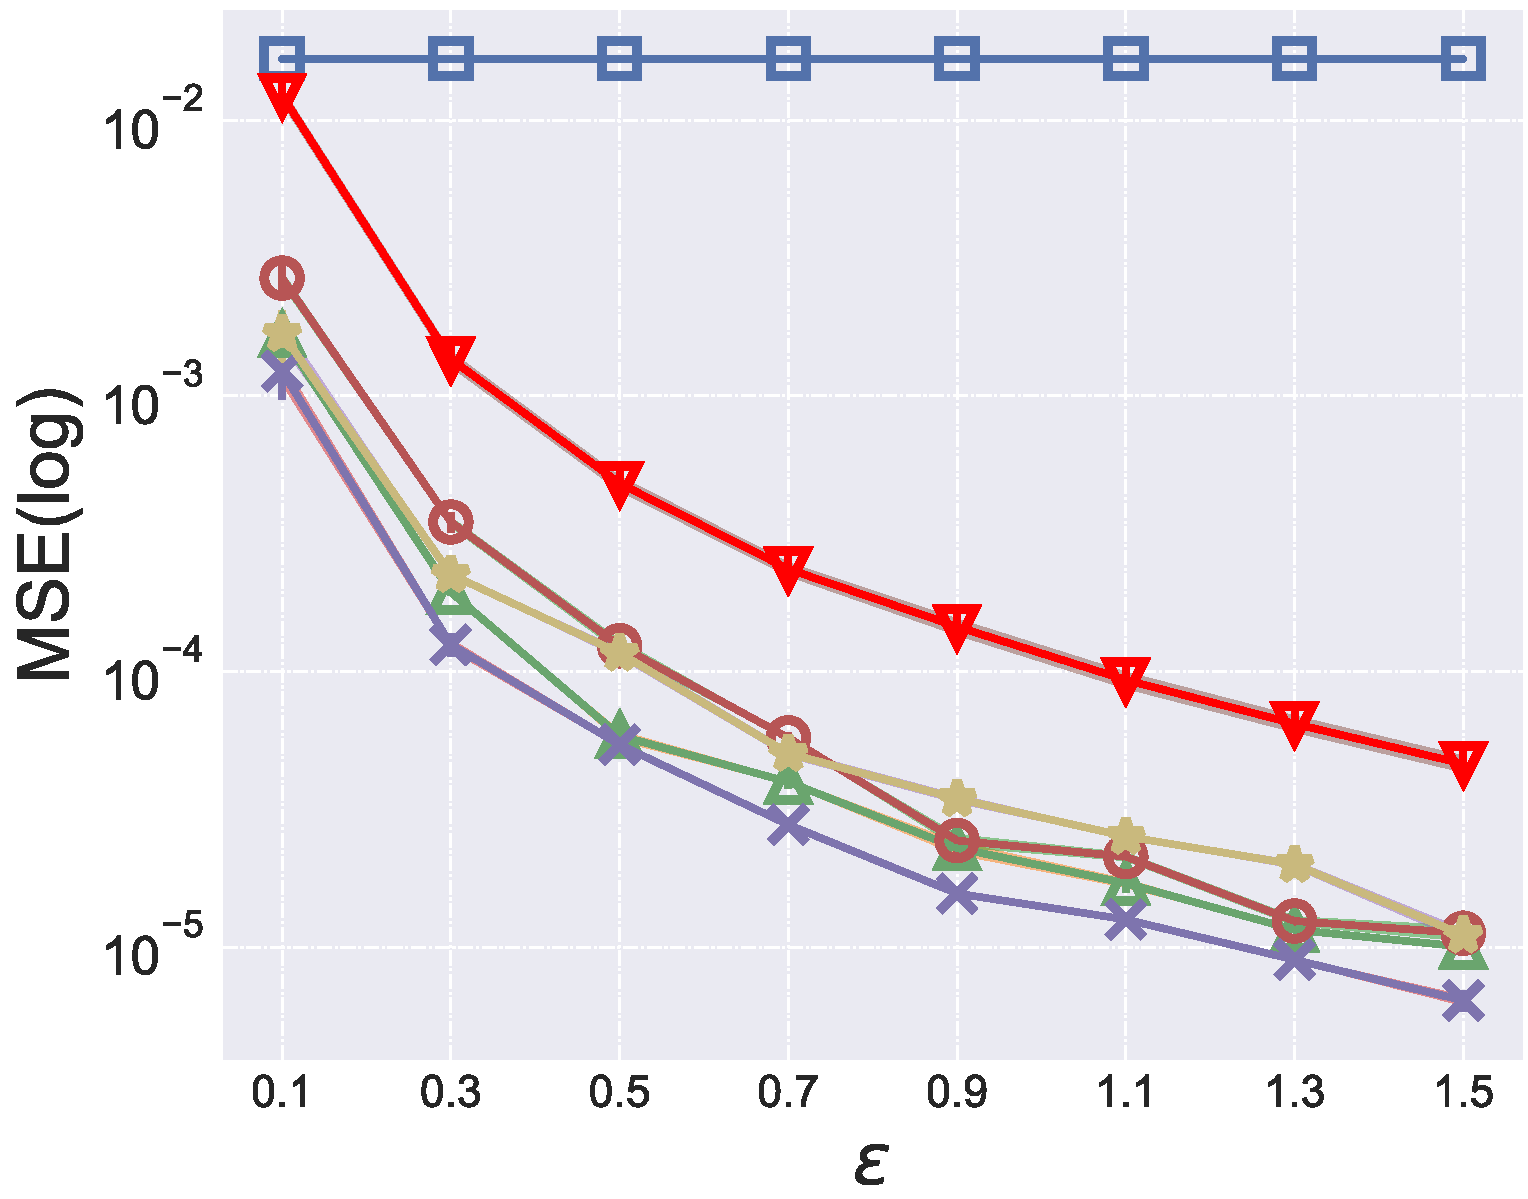
\includegraphics[width=0.23\hsize]{figure/ldp_range_query/figures_experiment_result/0531RandQuery/0404_CI_Rand_ep-Loan-Domain_2_8.pdf.pdf}
    }
    \subfigure[Financial, 512,  vary $\epsilon$]{
    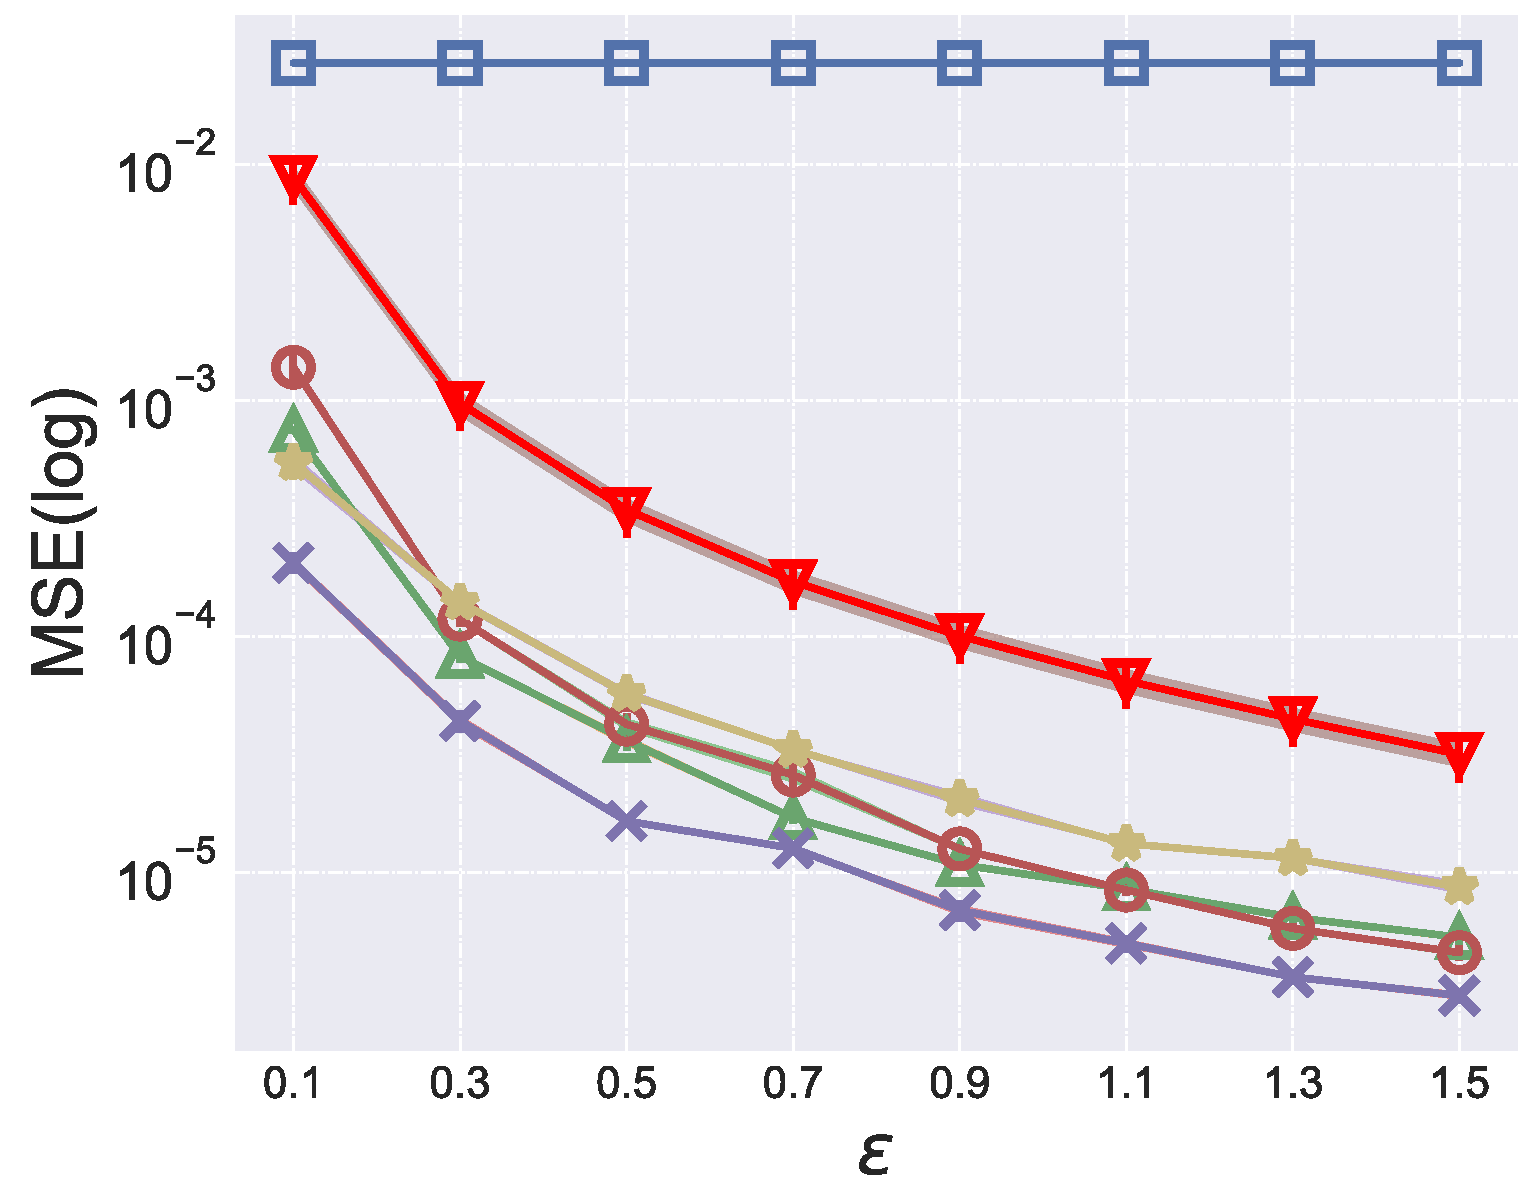
\includegraphics[width=0.23\hsize]{figure/ldp_range_query/figures_experiment_result/0531RandQuery/0404_CI_Rand_ep-Financial-Domain_2_9.pdf.pdf}
    }
    \subfigure[BlackFriday, 1028,  vary $\epsilon$]{
    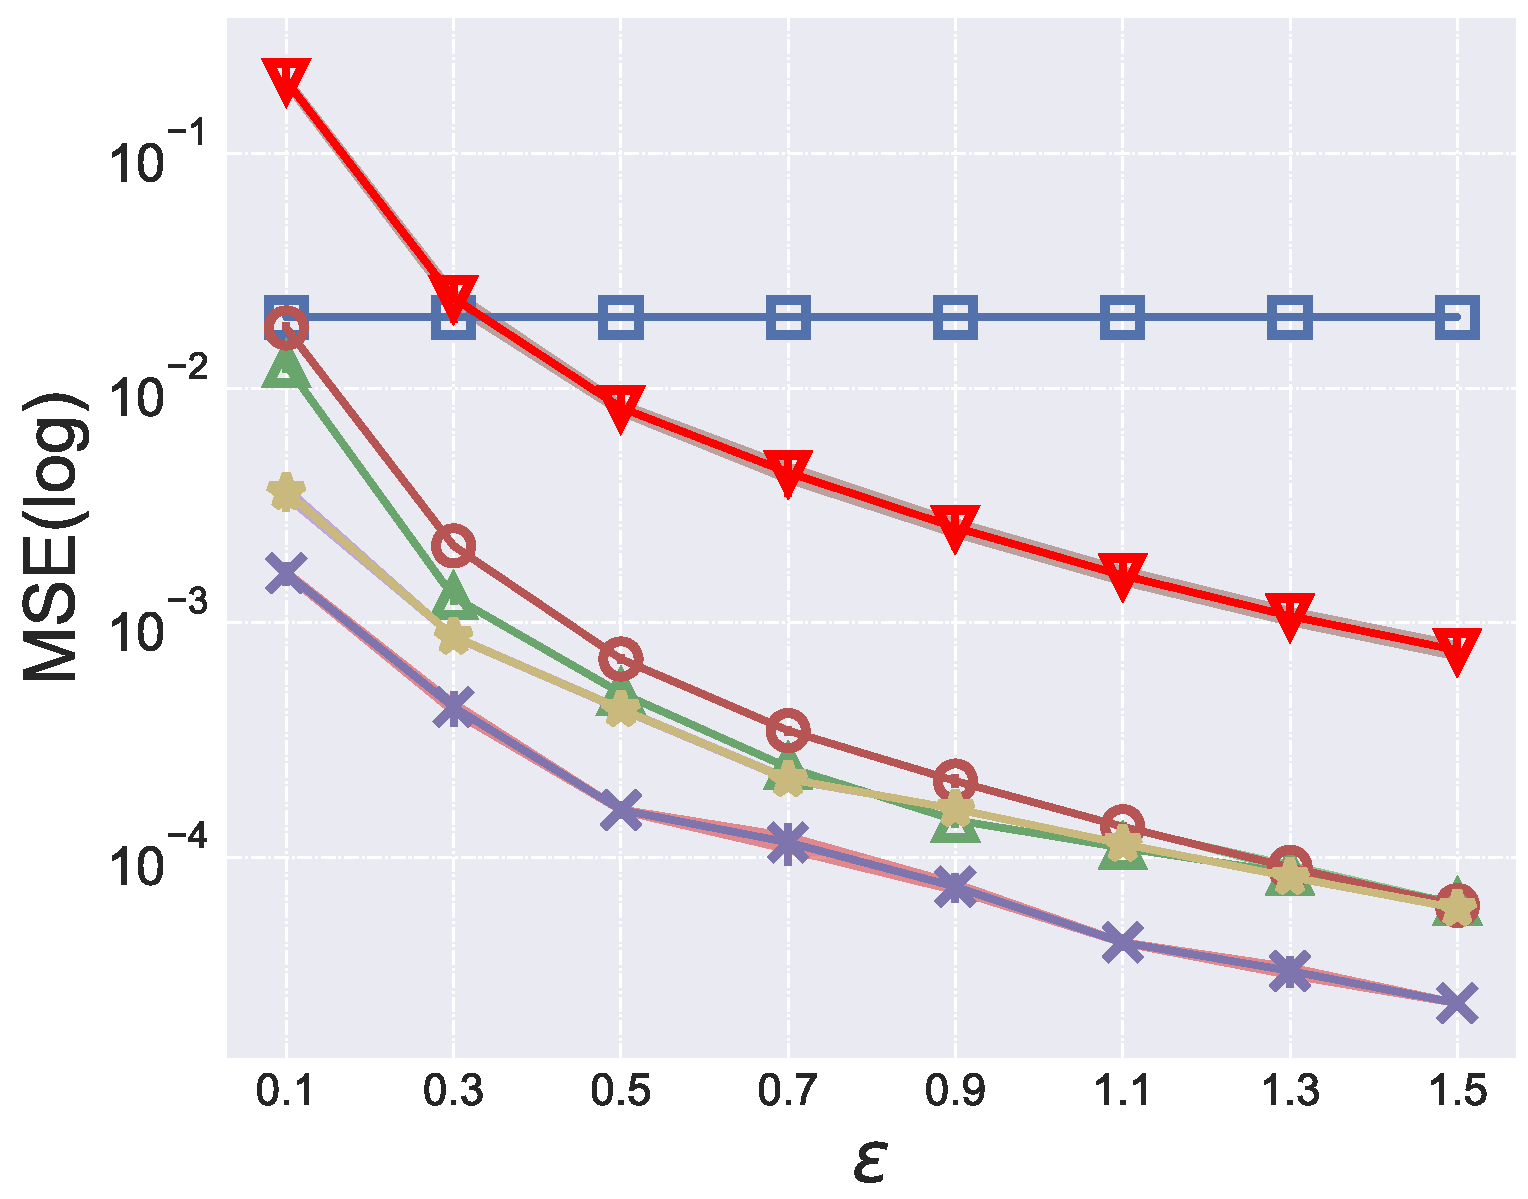
\includegraphics[width=0.23\hsize]{figure/ldp_range_query/figures_experiment_result/0531RandQuery/0404_CI_Rand_ep-BlackFriday-Domain_2_10.pdf.pdf}
    }
    \subfigure[Salaries, 2048,  vary $\epsilon$]{
    \label{overall compare Salaries}
    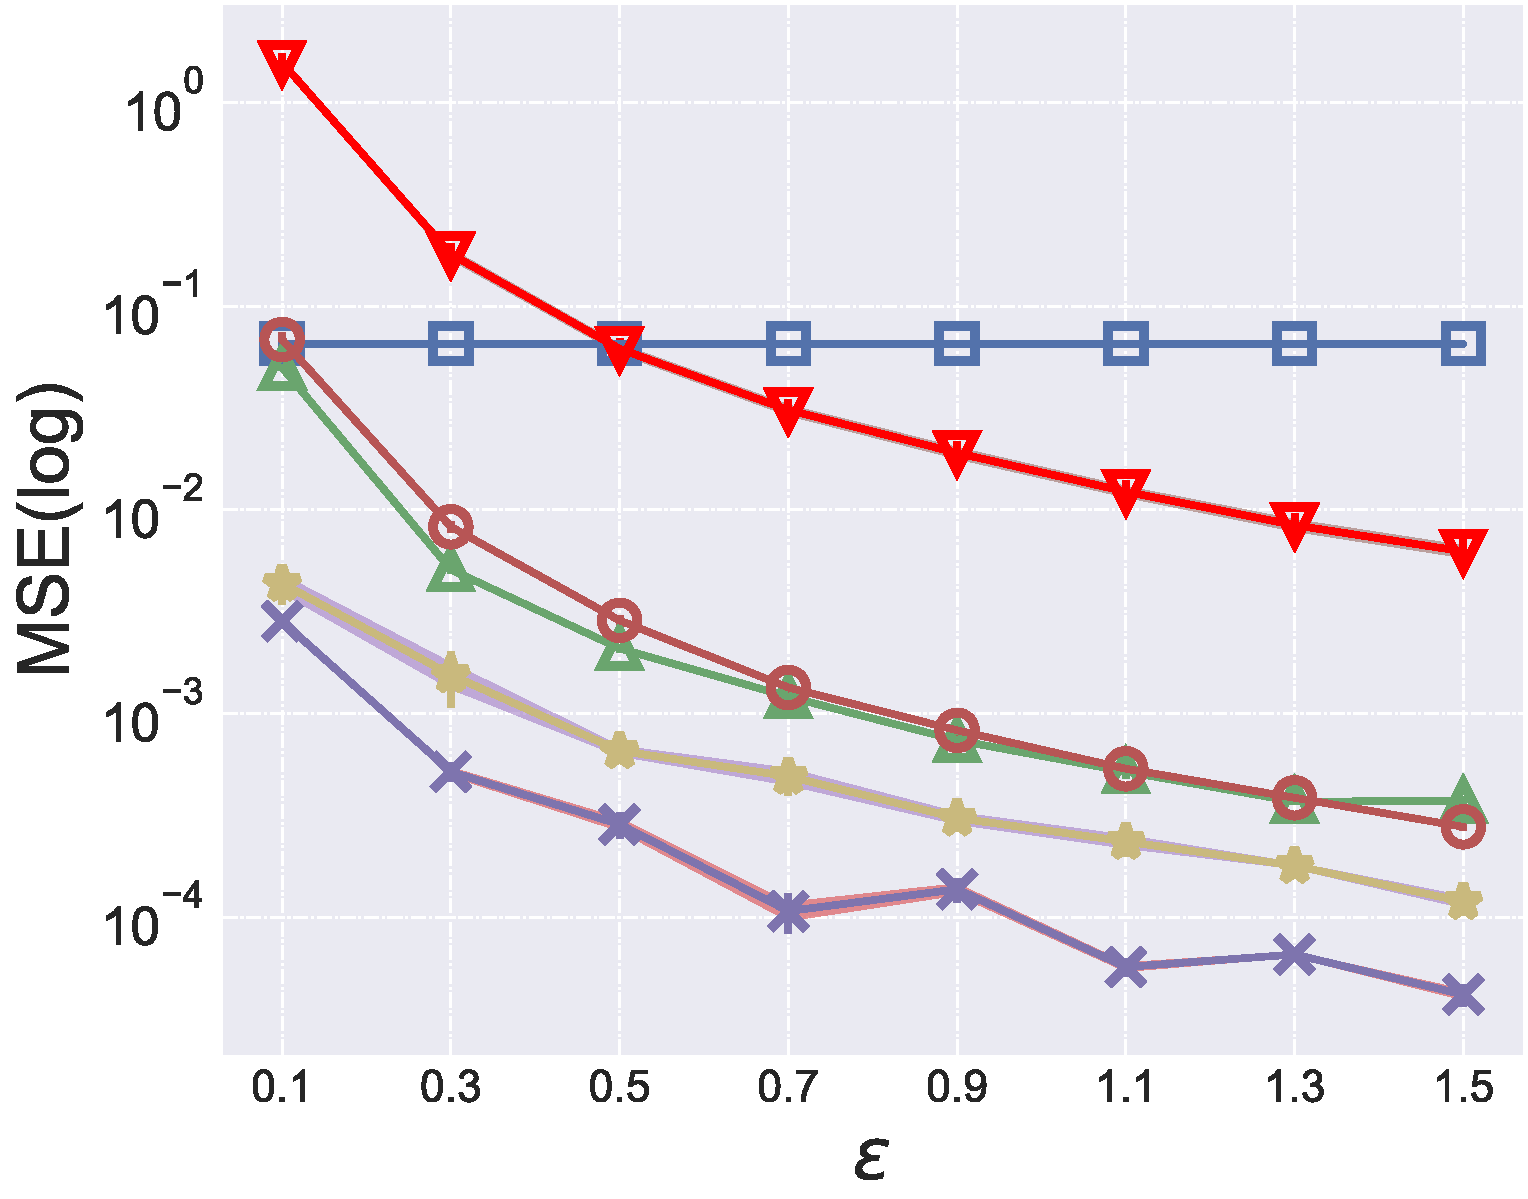
\includegraphics[width=0.23\hsize]{figure/ldp_range_query/figures_experiment_result/0531RandQuery/0404_CI_Rand_ep-Salaries-Domain_2_11.pdf.pdf}
    }
    \\[-0.5ex]
    \subfigure{
    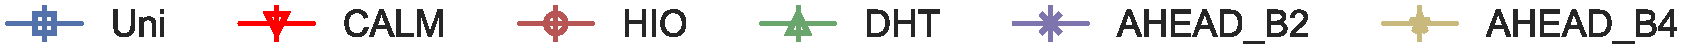
\includegraphics[width=0.8\hsize]{figure/ldp_range_query/figures_others/comparison_1D_legend6.pdf.pdf} 
    }
    \vspace{-0.2cm}
    \caption{不同方法的MSE,隐私预算从0.1到1.5变化,结果以对数刻度显示。}
    \label{overall compare}
\end{figure*}

我们在多种隐私预算条件下评估\myahead 的有效性。
具体来说,我们将隐私预算$\epsilon$从0.1(表示高隐私保护强度)变化到1.5(表示低隐私保护强度)进行考虑\cite{zhang2018calm, cormode2019answering}。 
\autoref{overall compare}展示了\myahead 与现有文献{\rm\parencite{cormode2019answering, wang2019answering, zhang2018calm}}在一维查询中的MSE比较。
对于每个图,我们在横轴上变化隐私预算$\epsilon$,并在纵轴上展示其相应的MSE。
每个图中的直方图显示20次重复实验MSE的平均值,误差线表示MSE的标准差。

从\autoref{overall compare}中,我们得出以下结论。
1)\myahead 的MSE始终比其他算法小。
回顾\autoref{Selection parameters}中的\autoref{theta setting 2},对于频率值低于阈值的节点,\myahead 采用自适应策略比采用基线策略的对比方法具有更小的总体估计误差。
2)\myahead 在不同数据集上表现不同。对于Salaries数据集,\myahead 在整个隐私预算范围内都比之前的方法显著优越,其中\myahead 的MSE几乎比现有方法小一个数量级。
对于Loan数据集,\myahead 略优于\mydht。
主要是因为这两个数据集具有完全不同的分布特性,
例如Salaries数据集上有更多频率值小于阈值的子域,
而Loan数据集则相对较少,使得\myahead 在这两个数据集上表现不同。


\subsection{二维数据场景}
\begin{figure*}[h!]
    \centering
    \subfigure[\Laplacian, $256^2$, vary $\epsilon$]{\label{fig:Two_Laplace08-Set_10_7-Domain_8_8}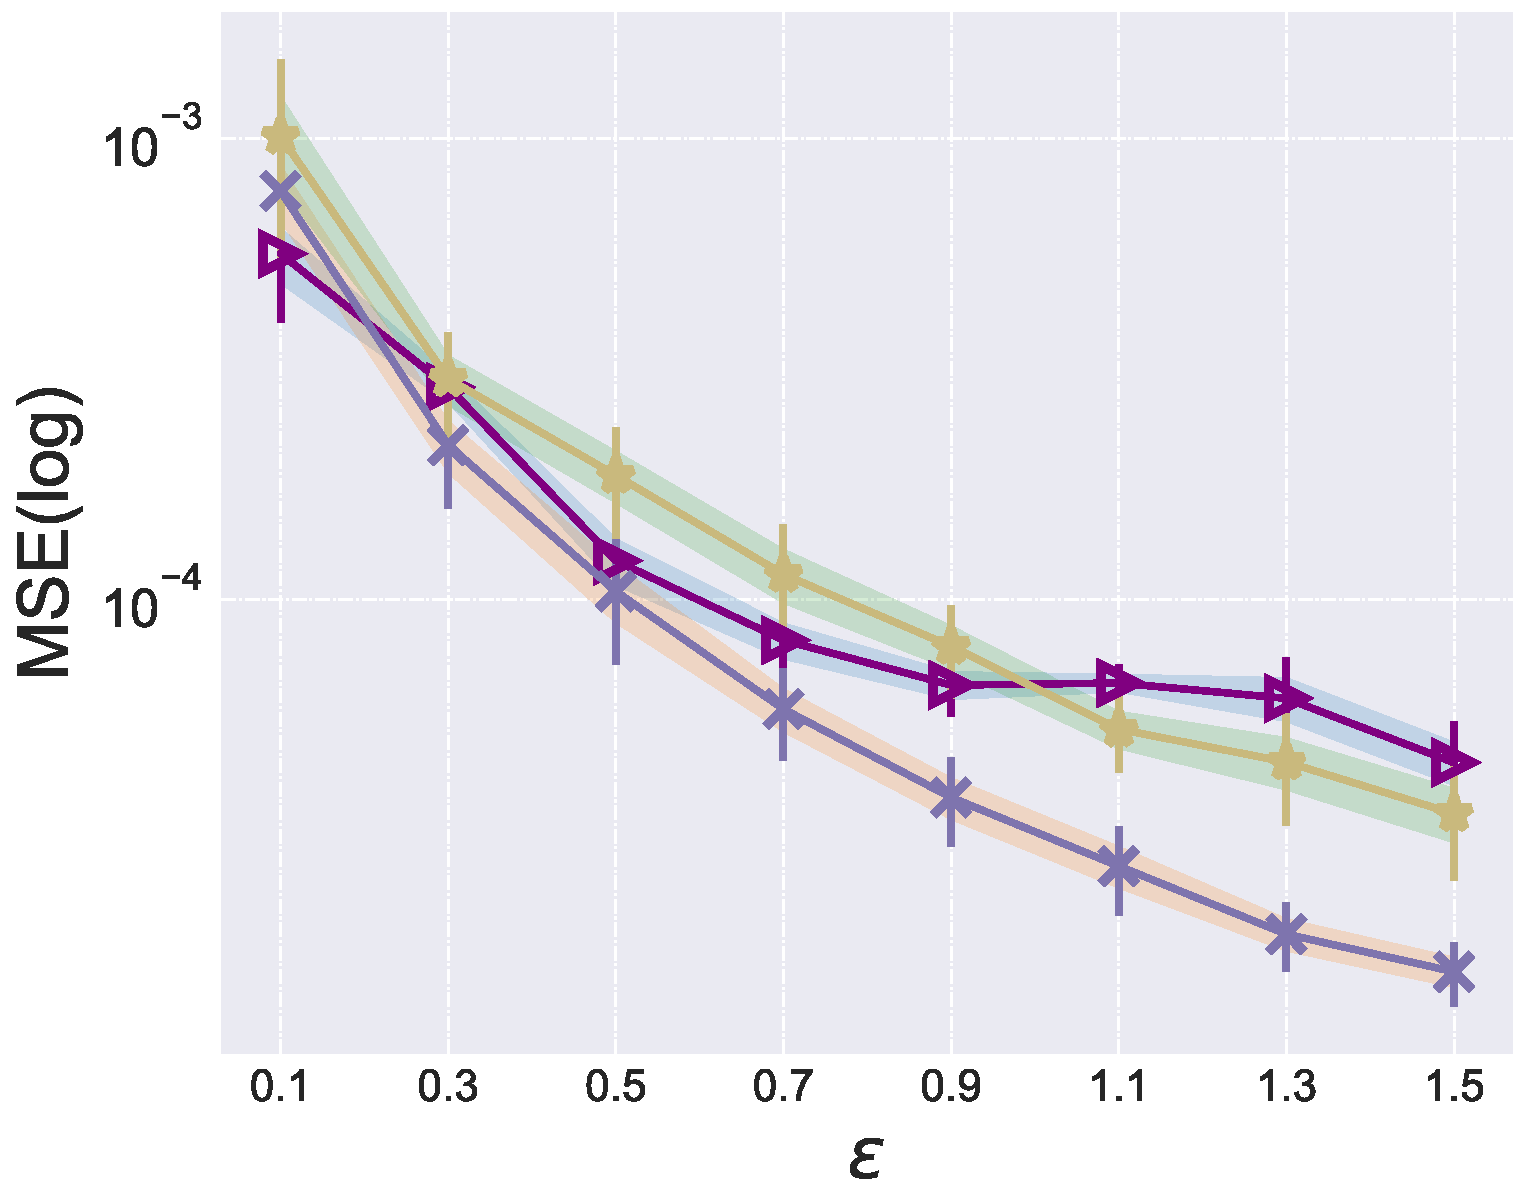
\includegraphics[width=0.24\hsize]{figure/ldp_range_query/figures_experiment_result/overall_result/20210404_CI_Rand_ep-Two_Laplace08-Set_10_7-Domain_8_8.pdf.pdf}}
    \subfigure[\Laplacian, $1024^2$, vary $\epsilon$]{\label{fig:Two_Laplace08-Set_10_7-Domain_10_10}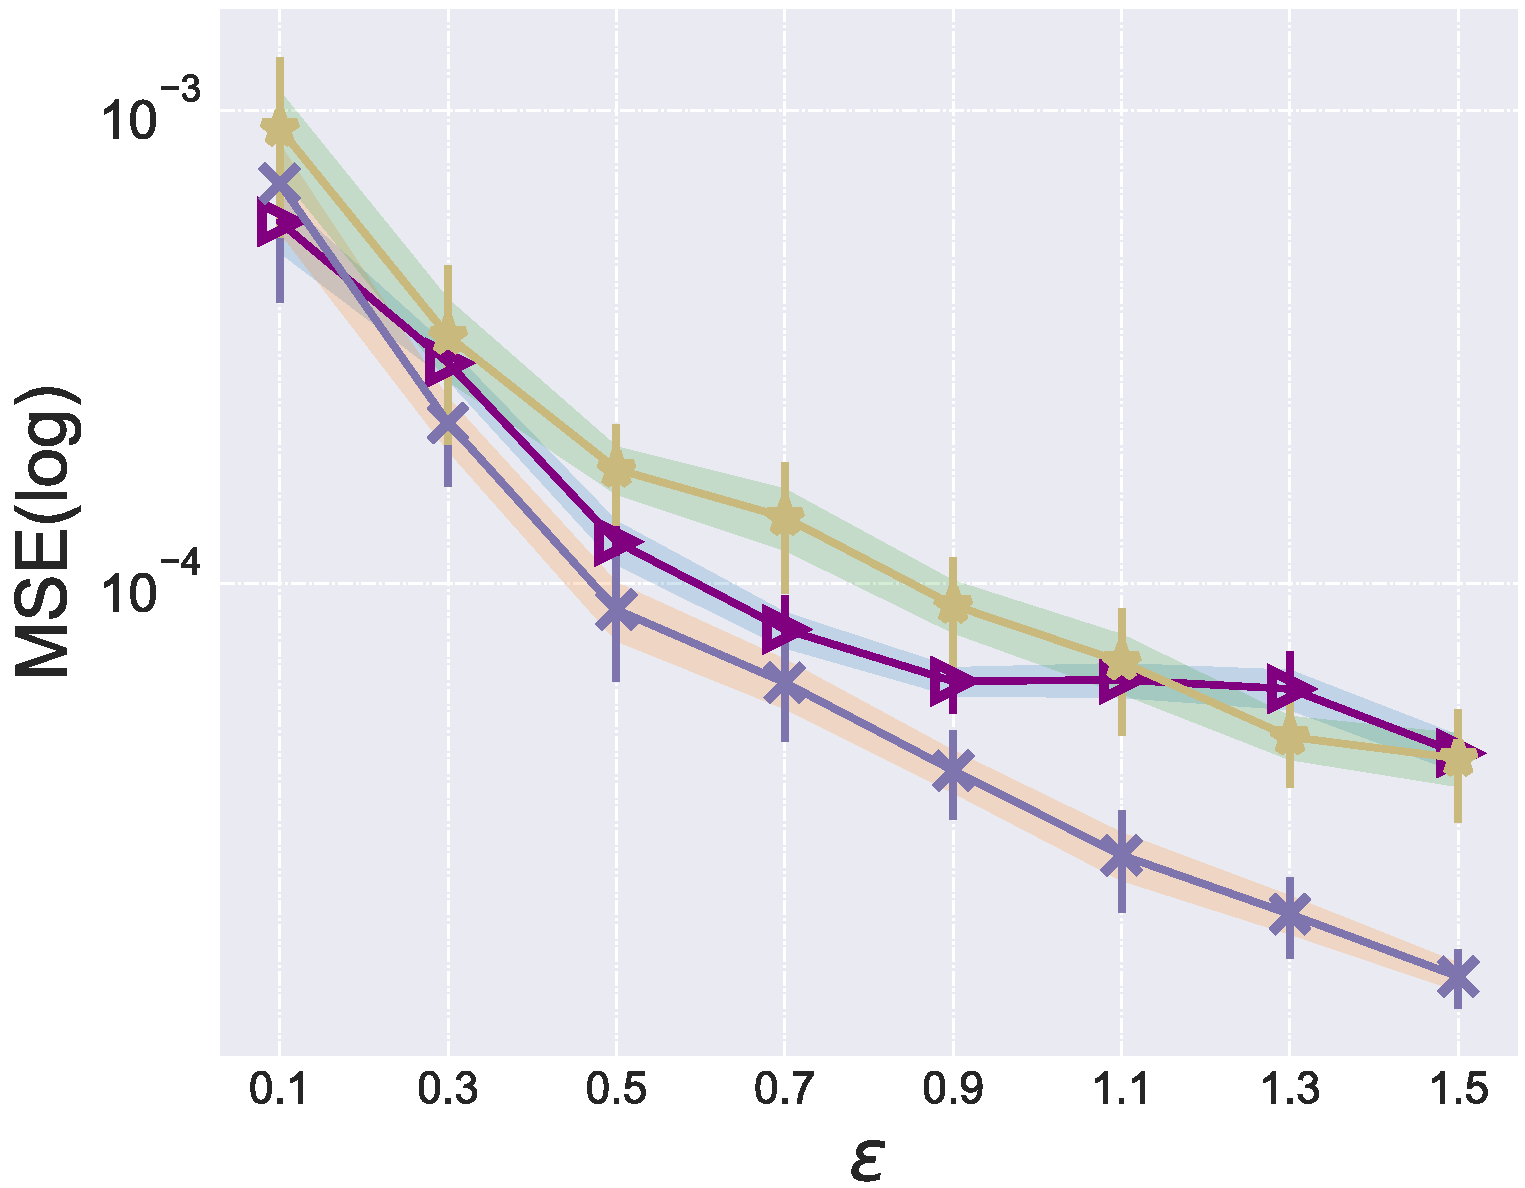
\includegraphics[width=0.24\hsize]{figure/ldp_range_query/figures_experiment_result/overall_result/20210404_CI_Rand_ep-Two_Laplace08-Set_10_7-Domain_10_10.pdf.pdf}}
    \subfigure[\Gaussian, $256^2$, vary $\epsilon$]{\label{fig:Two_Normal08-Set_10_7-Domain_8_8}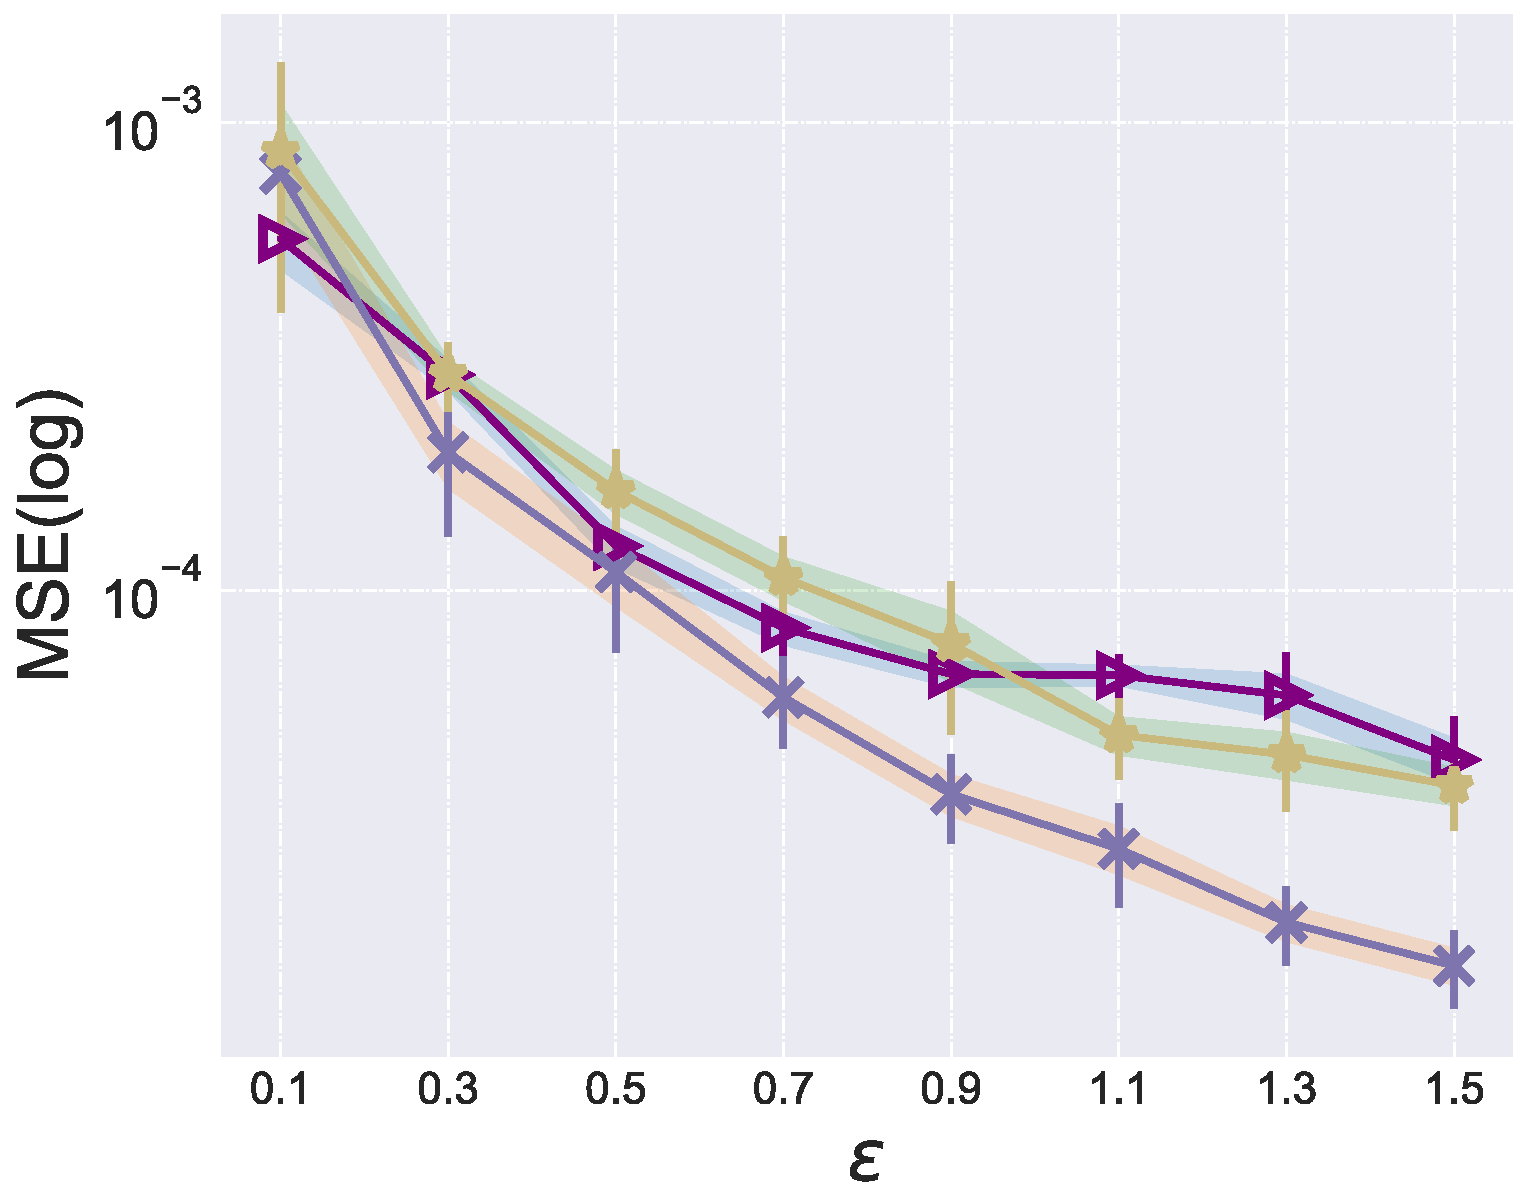
\includegraphics[width=0.24\hsize]{figure/ldp_range_query/figures_experiment_result/overall_result/20210404_CI_Rand_ep-Two_Normal08-Set_10_7-Domain_8_8.pdf.pdf}}
    \subfigure[\Gaussian, $1024^2$, vary $\epsilon$]{\label{fig:Two_Normal08-Set_10_7-Domain_10_10}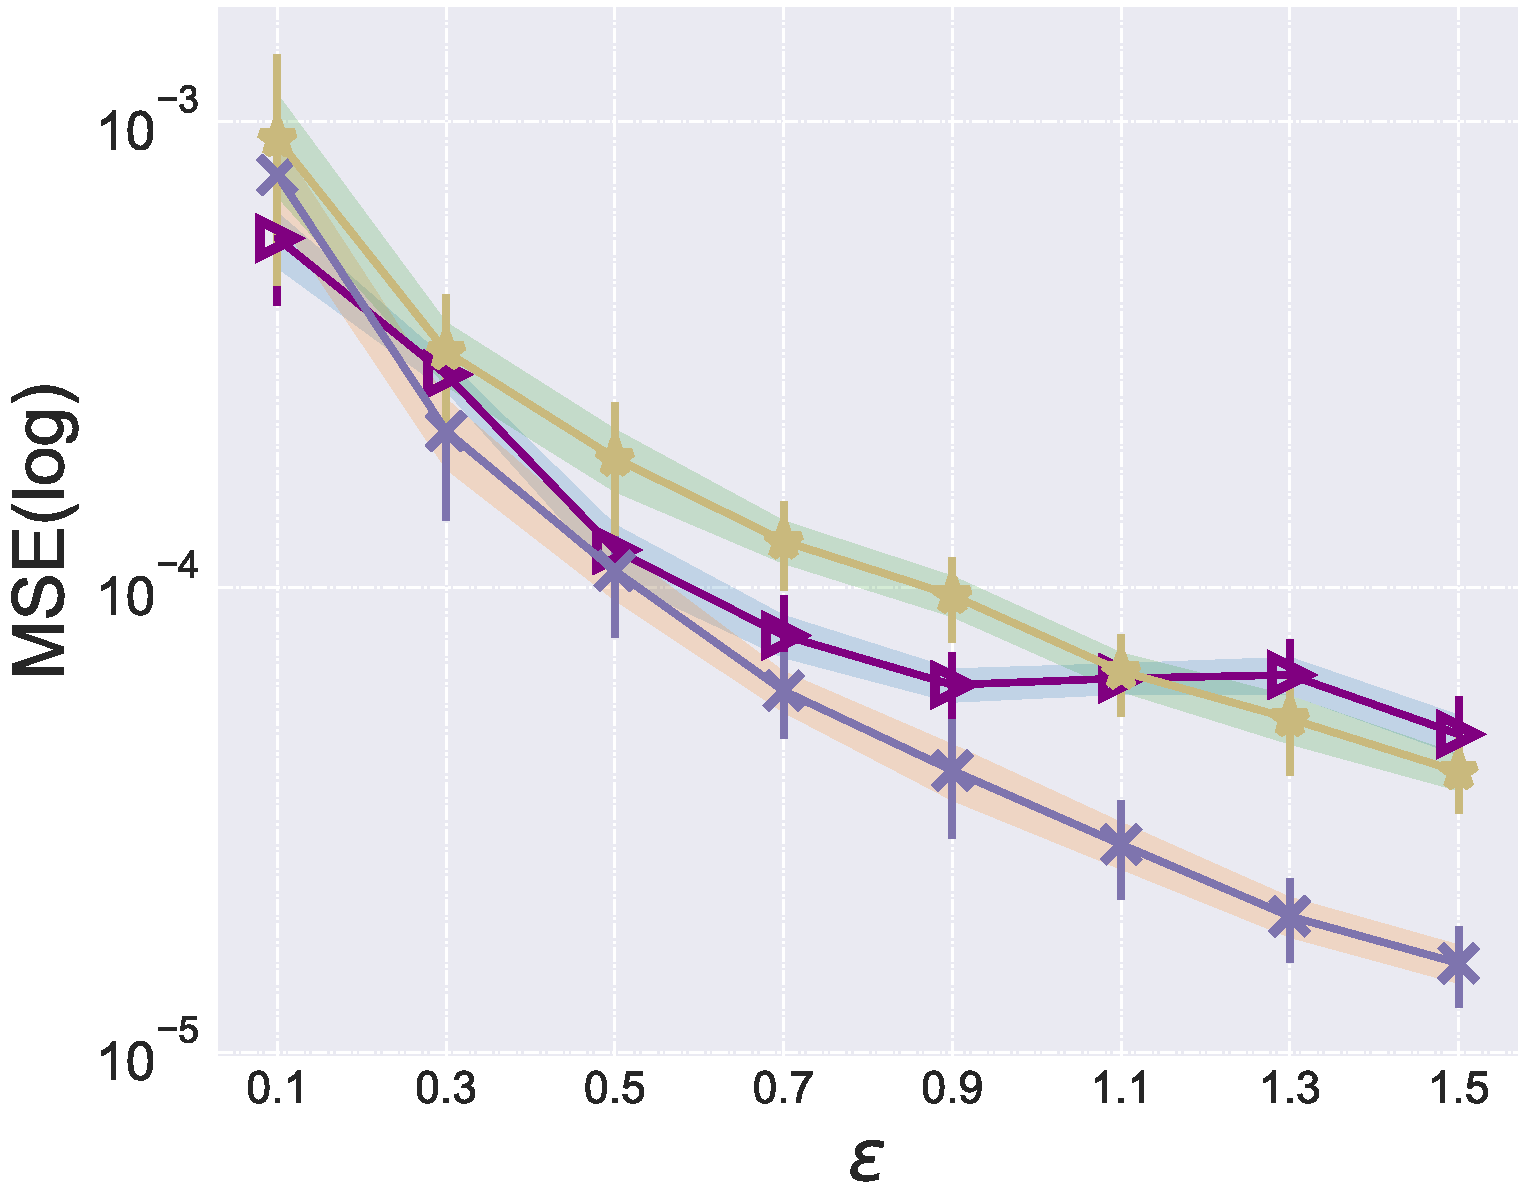
\includegraphics[width=0.24\hsize]{figure/ldp_range_query/figures_experiment_result/overall_result/20210404_CI_Rand_ep-Two_Normal08-Set_10_7-Domain_10_10.pdf.pdf}}
    \\[-0.5ex]
    \subfigure{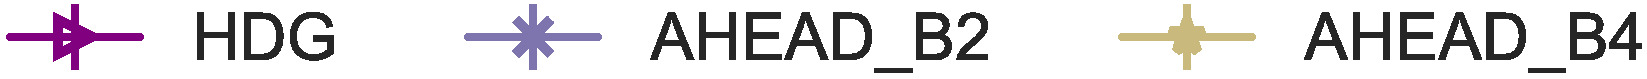
\includegraphics[width=0.4\textwidth]{figure/ldp_range_query/figures_others/comparison_2D_legend.pdf.pdf}} 
    \vspace{-0.2cm}
    \caption{
        % Comparison of different methods on \Laplacian and \Gaussian datasets under various privacy budgets. We only plot the methods that are scalable in each setting. \myHDG is a baseline method. The results are shown in log scale.
        基于\Laplacian 和 \Gaussian 数据集,我们比较了\myahead 和现有方法在不同隐私预算下的性能,结果以对数刻度显示。其中,\myHDG 是基准方法。}
    % \vspace{-0.5cm}
    \label{2-dim overall compare}
\end{figure*}

\begin{figure*}[h!]
    \centering
    \subfigure[\Laplacian, $256^2$, vary $r$]{\label{fig:Two_Laplace08-Set_10_7-Domain_8_8}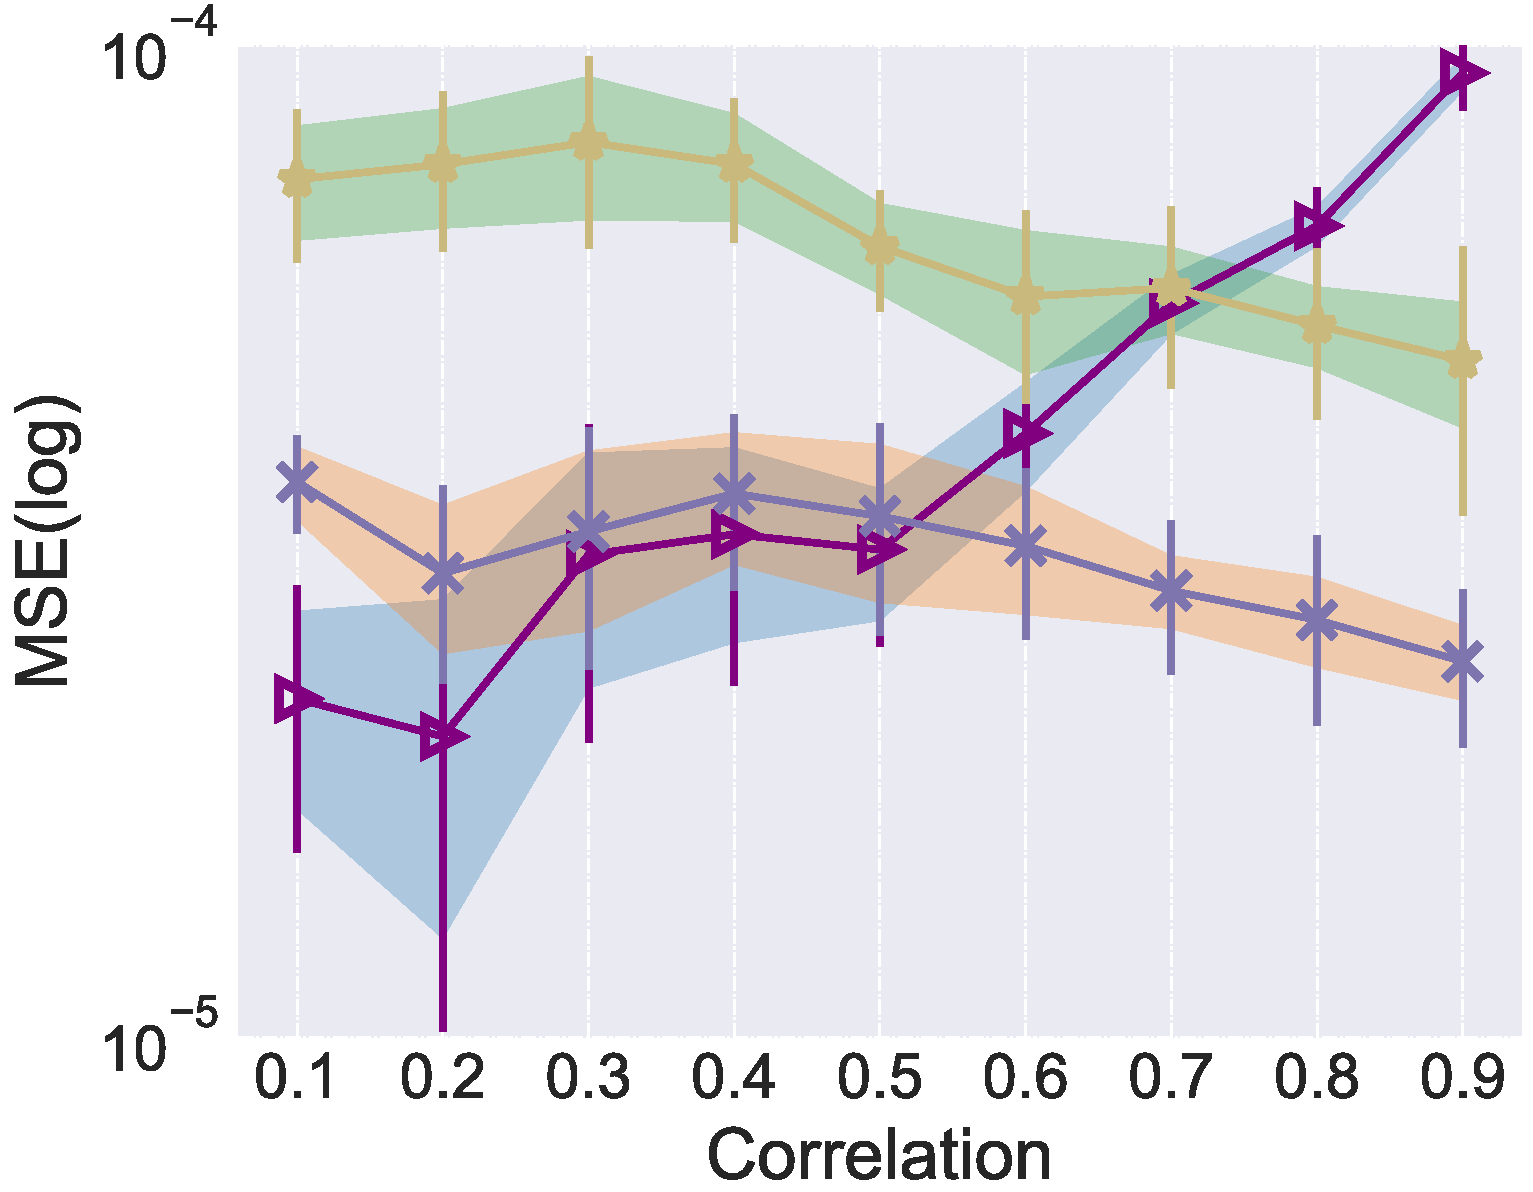
\includegraphics[width=0.24\hsize]{figure/ldp_range_query/figures_experiment_result/overall_result/20210404Correlation-Two_Laplace-Set_10_7-Domain_8_8.pdf.pdf}}
    \subfigure[\Laplacian, $1024^2$, vary $r$]{\label{fig:Two_Laplace09-Set_10_7-Domain_8_8}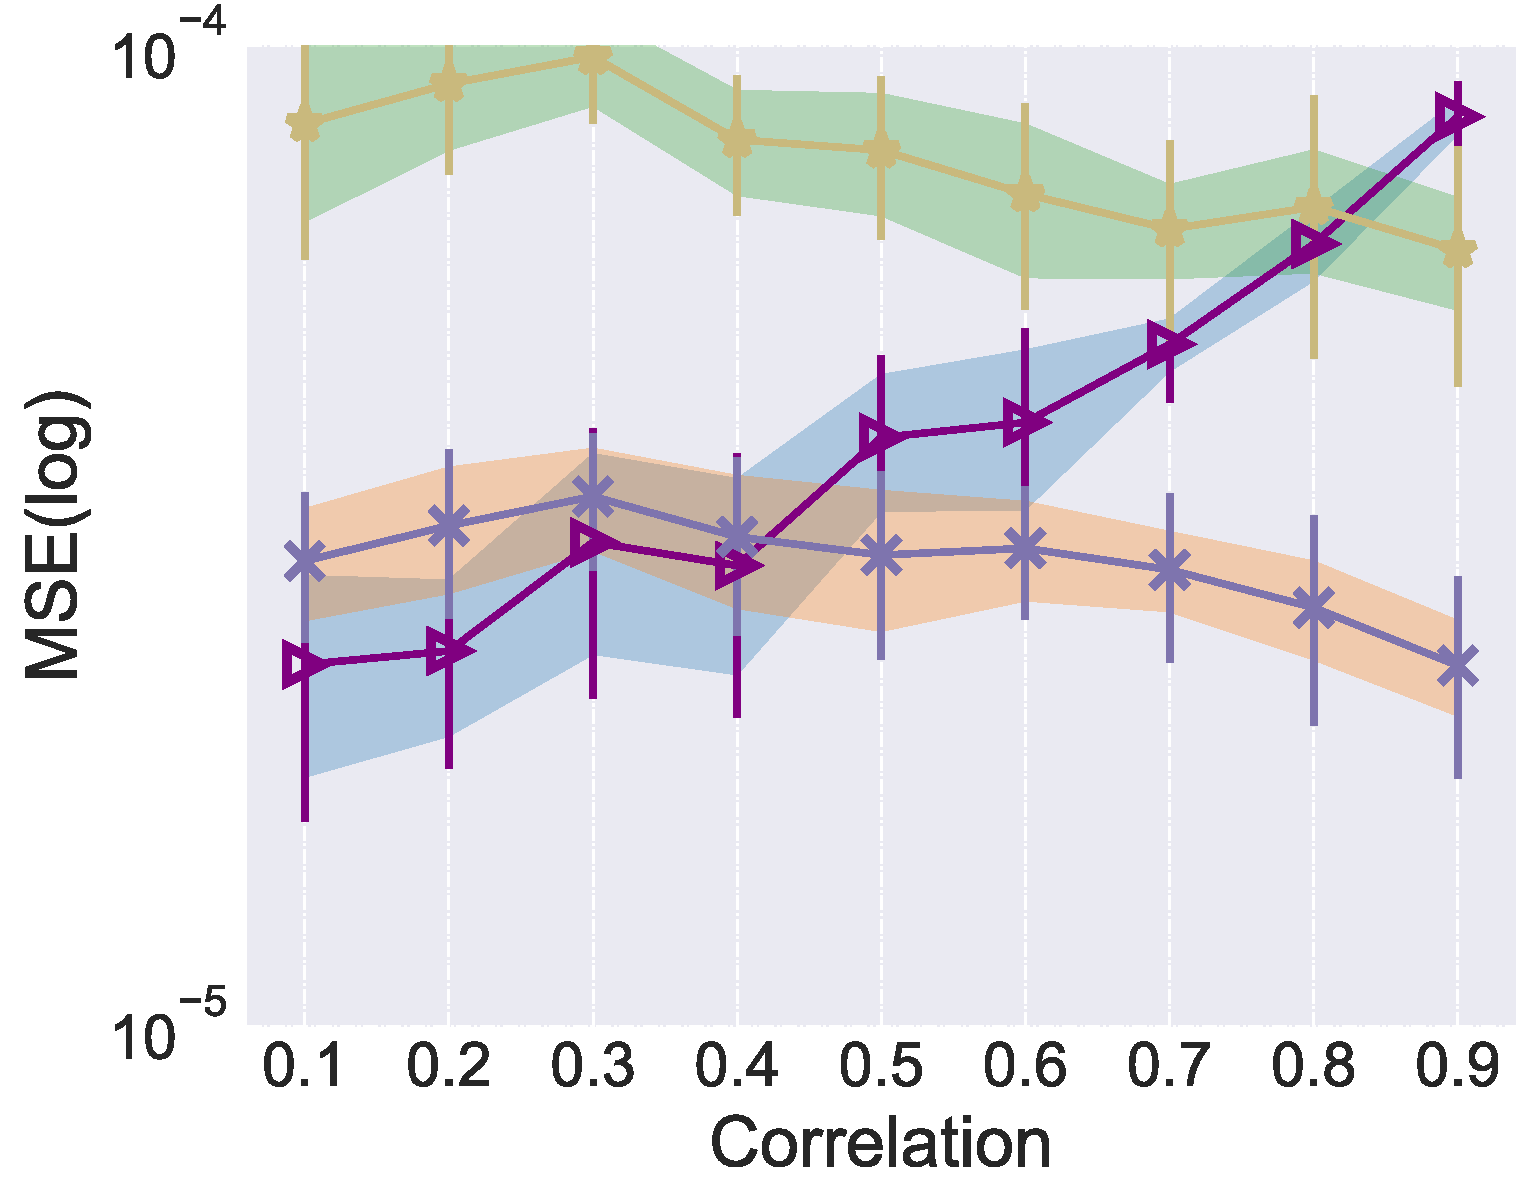
\includegraphics[width=0.24\hsize]{figure/ldp_range_query/figures_experiment_result/overall_result/20210404Correlation-Two_Laplace-Set_10_7-Domain_10_10.pdf.pdf}}
    \subfigure[\Gaussian, $256^2$, vary $r$]{\label{fig:Two_Laplace08-Set_10_7-Domain_10_10}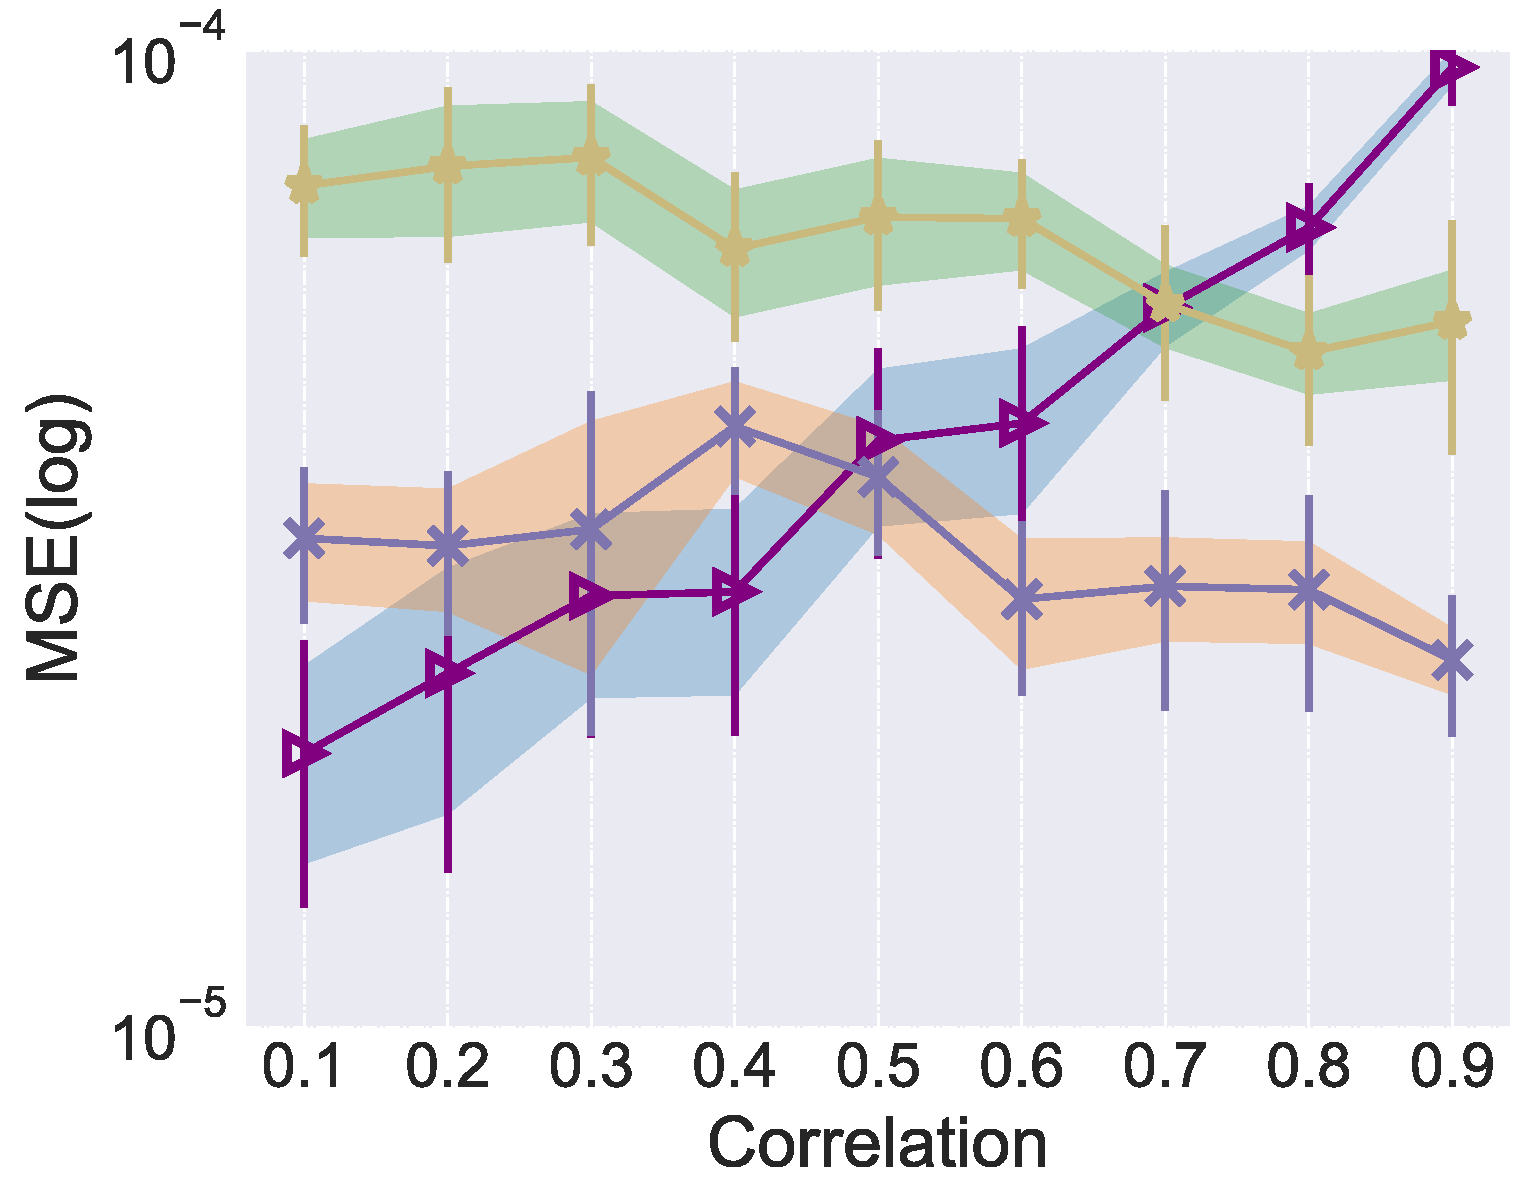
\includegraphics[width=0.24\hsize]{figure/ldp_range_query/figures_experiment_result/overall_result/20210404Correlation-Two_Normal-Set_10_7-Domain_8_8.pdf.pdf}}
    \subfigure[\Gaussian, $1024^2$, vary $r$]{\label{fig:Two_Laplace09-Set_10_7-Domain_10_10}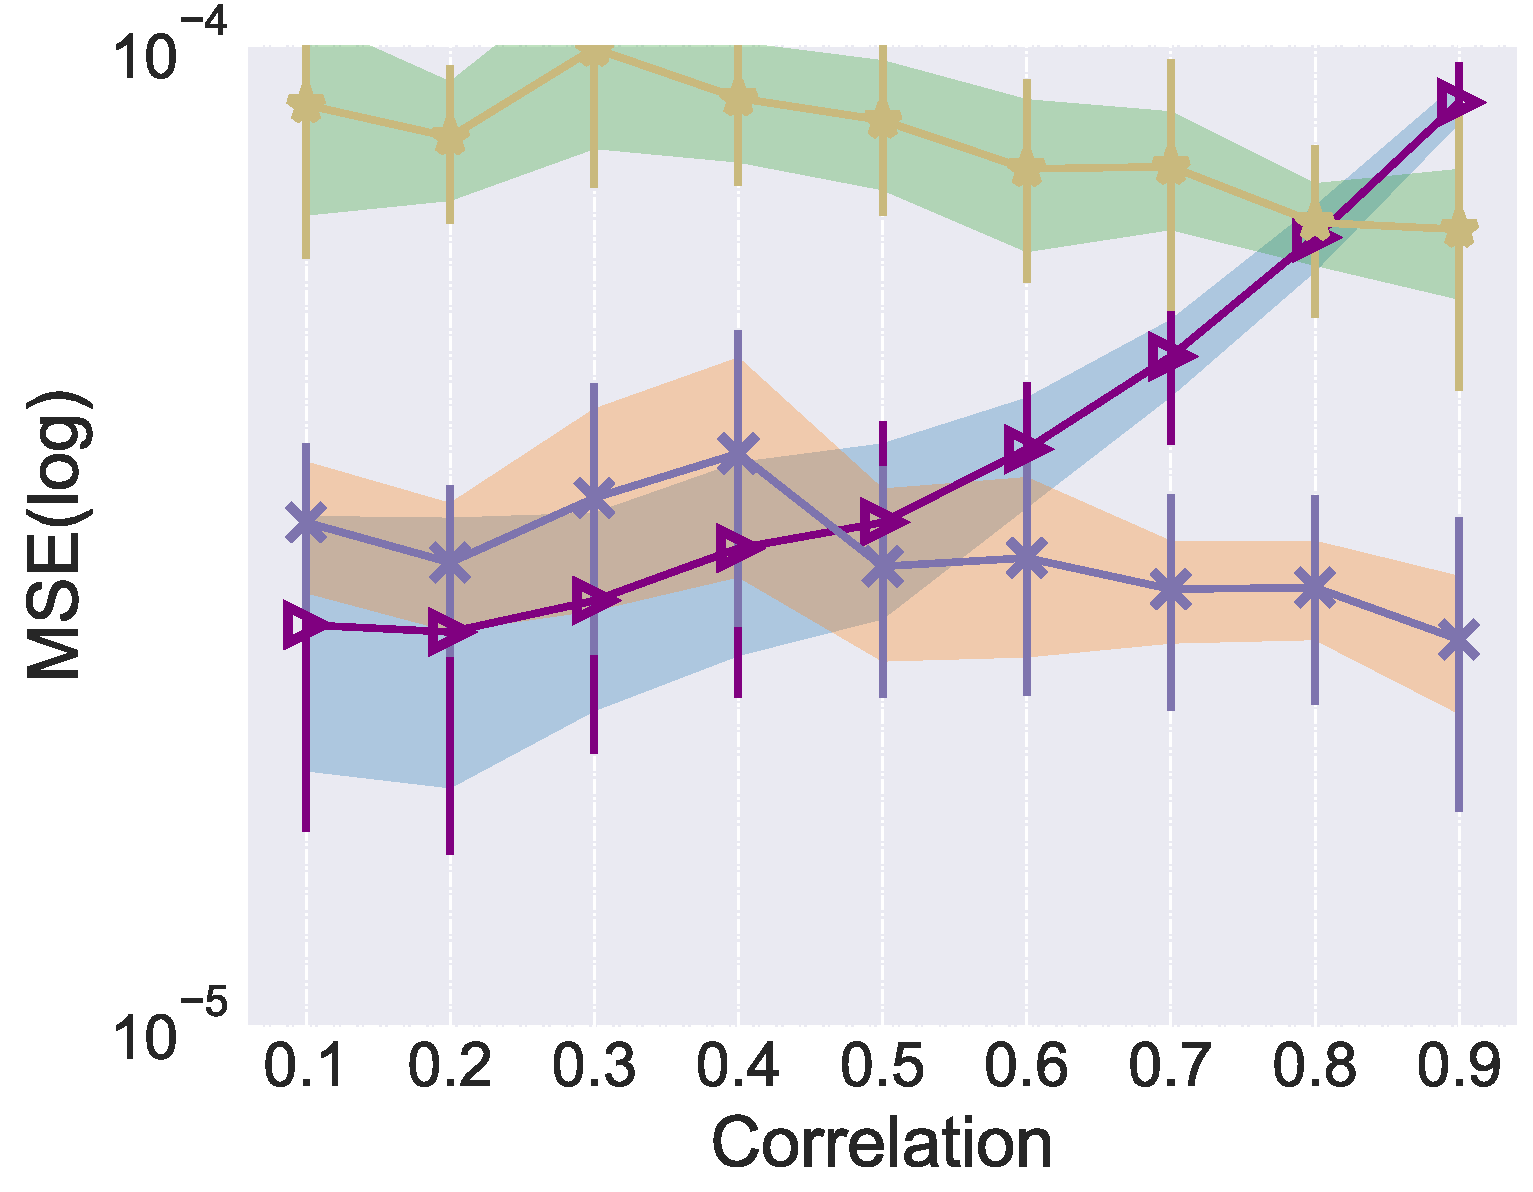
\includegraphics[width=0.24\hsize]{figure/ldp_range_query/figures_experiment_result/overall_result/20210404Correlation-Two_Normal-Set_10_7-Domain_10_10.pdf.pdf}}
    \\[-0.5ex]
    \subfigure{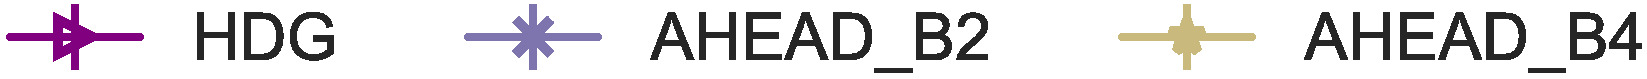
\includegraphics[width=0.4\textwidth]{figure/ldp_range_query/figures_others/comparison_2D_legend.pdf.pdf}}  
    \vspace{-0.2cm}
    \caption{基于\Laplacian 和 \Gaussian 数据集,我们比较了\myahead 和现有方法在不同属性相关性下的性能,结果以对数刻度显示。其中,\myHDG 是基准方法。}
    % \vspace{-0.5cm}
    \label{2-dim correlation}
\end{figure*}

\mypara{不同属性相关性下的算法查询精度}
我们评估了在二维查询下不同隐私预算对算法性能的影响。
% 在这里,我们专注于合成数据集,因为它们可以反映算法在标准分布上的性能,并有助于调整数据集参数。
每个数据集包含$10^7$条记录,分别从二维\Laplacian 分布和\Gaussian 分布中进行采样,
其中数据域大小分别为$256 \times 256$和$1024 \times 1024$。

\autoref{2-dim overall compare}展示了在二维\Laplacian 分布和\Gaussian 分布的结果。
我们采用与\cite{yang2020answering}相同的相关系数$r=0.8$。
由于\myuni 和\mycalm 的MSE超出了图表范围,因此我们省略了它们的结果。
根据结果,我们有以下观察结果。
1)在不同的隐私预算设置下,\myahead 表现优于\myHDG 。
\myHDG 利用粗粒度的二维网格对二维数据域进行划分,并刻画两个属性之间的相关信息。
当数据域大小为$1024 \times 1024$时,\myHDG 的最精细粒度是$8 \times 8$。
采用粗粒度的网格进行划分会导致数据相关性信息丢失。
相比之下,\myahead 针对具有不同频率值的子域使用多粒度分解方式。
对于一个用户数据集中分布的子域,\myahead 采用细粒度分解,以更准确地提取数据相关性。
2)\myahead 对于不同数据域大小具有鲁棒性。
一方面,更大的数据域意味着需要将用户划分为更多的组。
例如,对于$256 \times 256$的数据域,\myahead 将用户划分为8组。
而对于$1024 \times 1024$的数据域,\myahead 将用户划分为10组。
对于更大的数据域,每个组中的用户数量较少,这将增加频率值中添加的噪声。
另一方面,频率小于阈值的子域不会被进一步划分。
我们使用多个用户组的上传数据估计这些子域的频率值。
在后向处理中进行加权平均处理后,这些子域的噪声误差将变为原始噪声误差的$\frac{1}{\beta}$,其中$\beta$是估计次数。
% 通过比较\autoref{2-dim overall compare}中的两个相邻子图,阈值设置的影响比域大小变化的影响更大。因此,\myahead的MSE几乎不随不同域大小变化而变化,我们选择不同的域大小来进一步验证这一事实,详见\autoref{Impact of Domain Size}。

\mypara{不同属性相关性下的算法查询精度}
我们在\autoref{2-dim correlation}中展示了在不同属性相关性下查询误差。
在每个子图中,我们使用固定的隐私预算$\epsilon=1.1$,并将相关系数$r$从0.1(弱相关)变化到0.9(强相关)。
基于实验结果,我们总结出以下结论。
1)\myahead 的MSE几乎不随属性相关性而改变。
\myahead 同时分解了两个维度,因此更好地保护了数据的相关性。
2)\myHDG 的数据效用会随着属性相关性的增加而降低,特别是在属性相关性较强的情况下。
\myHDG 结合了更细粒度的一维网格来估计频率分布。
如果两个属性之间的相关性较弱,细粒度的一维网格可以弥补粗粒度的二维网格的精度不足的缺陷。
当属性之间的相关性较强时,缺少属性相关性信息的一维网格可能会对查询精度造成负面影响。
% 有趣的是,相关系数$r=0.5$似乎是\myHDG 和\myahead 的交点,这可能引导聚合器根据属性的相关性选择更好的算法。
% 对于高维场景,我们还在\autoref{Impact of Attribute Correlation}中评估了不同属性相关性对查询误差的影响,其中\myahead 的反应与二维场景类似。

\subsection{高维数据场景}
\label{Effectiveness of ahead for high-dimensional Range Query}
\begin{figure*}[h!]
    \centering
    \subfigure[\Laplacian~(3), $10^6$, vary $\epsilon$]{\label{fig:Three_Laplace08-Set_10_6-Domain_6_6_6}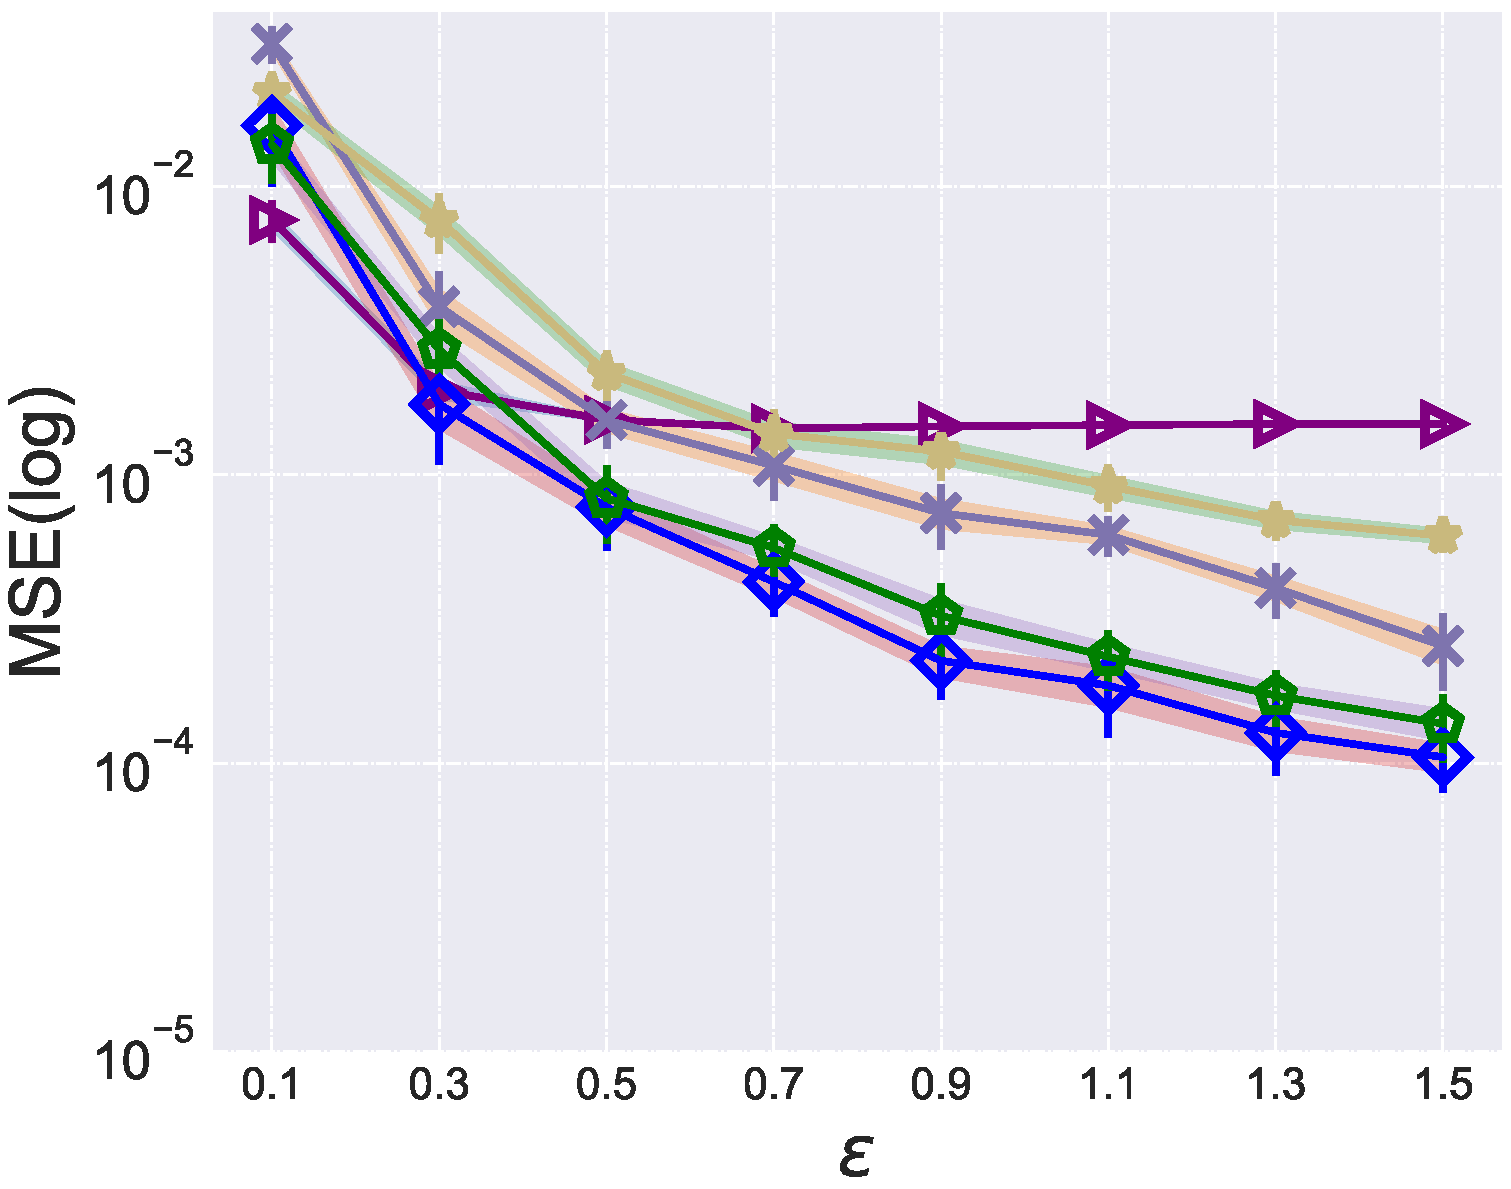
\includegraphics[width=0.24\hsize]{figure/ldp_range_query/figures_experiment_result/overall_result/0406_CI_Rand_ep-Three_Laplace08-Set_10_6-Domain_6_6_6.pdf.pdf}}
    \subfigure[\Laplacian~(3), $10^7$, vary $\epsilon$]{\label{fig:Three_Laplace08-Set_10_7-Domain_6_6_6}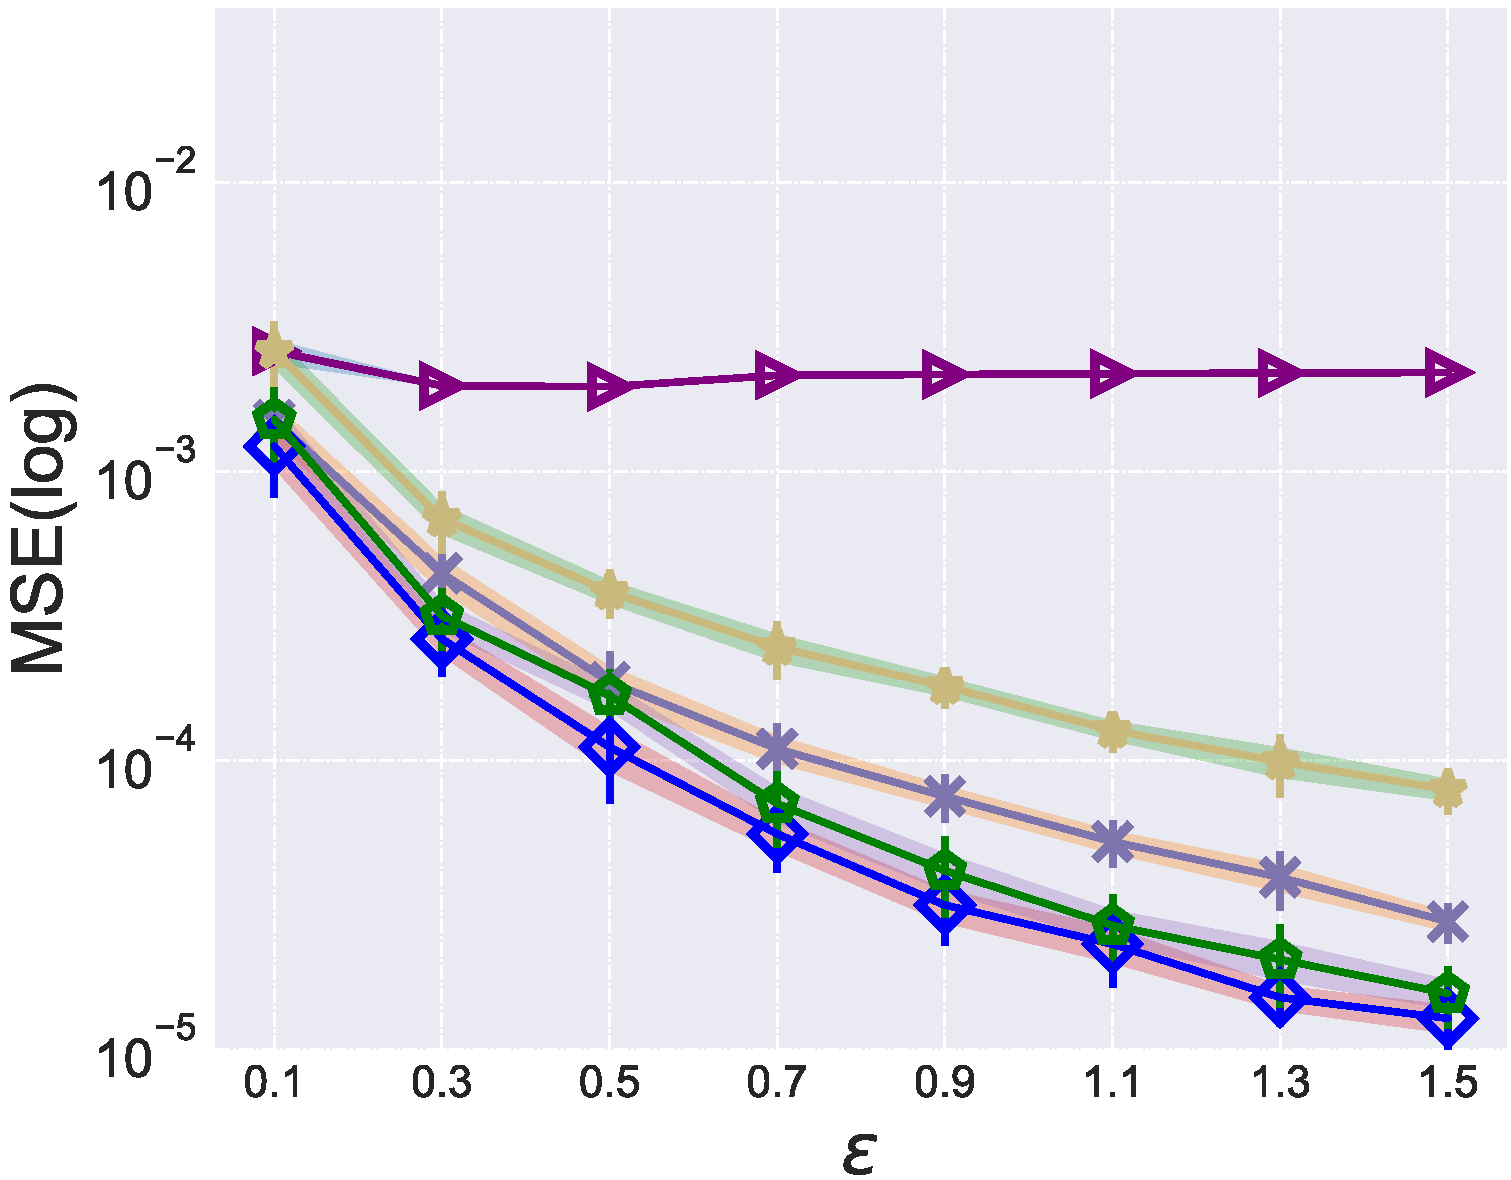
\includegraphics[width=0.24\hsize]{figure/ldp_range_query/figures_experiment_result/overall_result/0406_CI_Rand_ep-Three_Laplace08-Set_10_7-Domain_6_6_6.pdf.pdf}}
    \subfigure[\Gaussian~(3), $10^6$, vary $\epsilon$]{\label{fig:Three_Normal08-Set_10_6-Domain_6_6_6}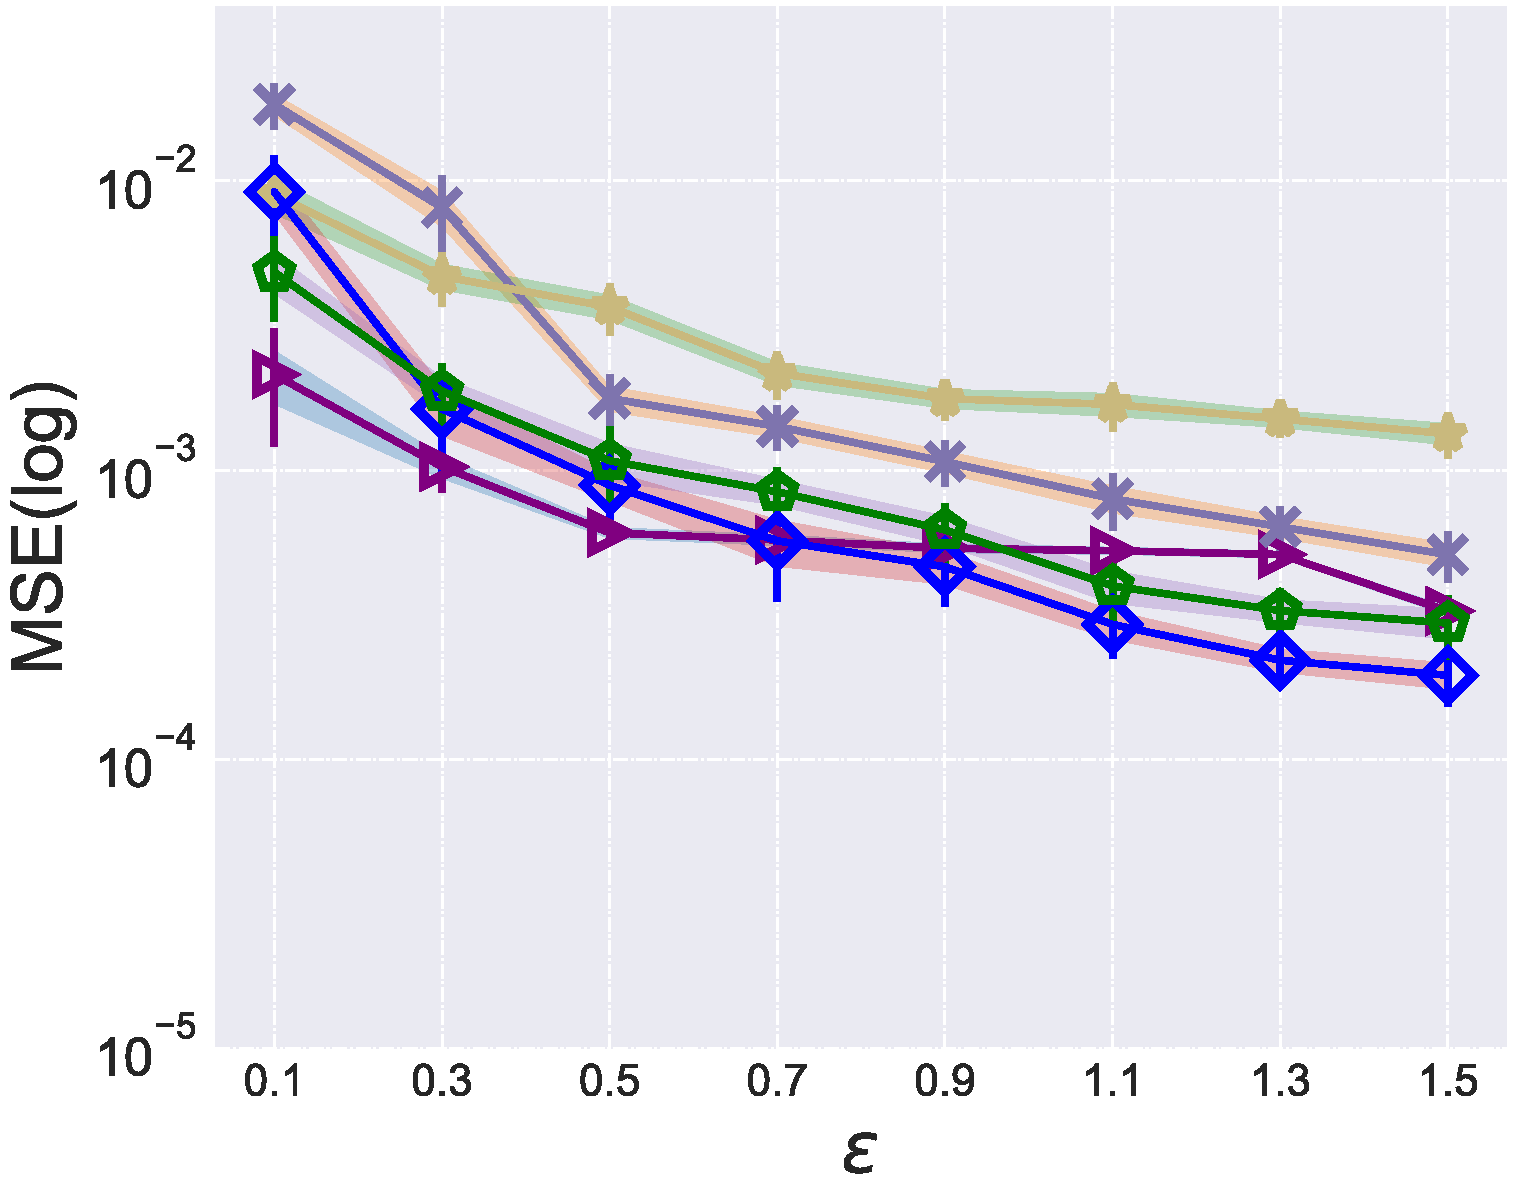
\includegraphics[width=0.24\hsize]{figure/ldp_range_query/figures_experiment_result/overall_result/0406_CI_Rand_ep-Three_Normal08-Set_10_6-Domain_6_6_6.pdf.pdf}}
    \subfigure[\Gaussian~(3), $10^7$, vary $\epsilon$]{\label{fig:Three_Normal08-Set_10_7-Domain_6_6_6}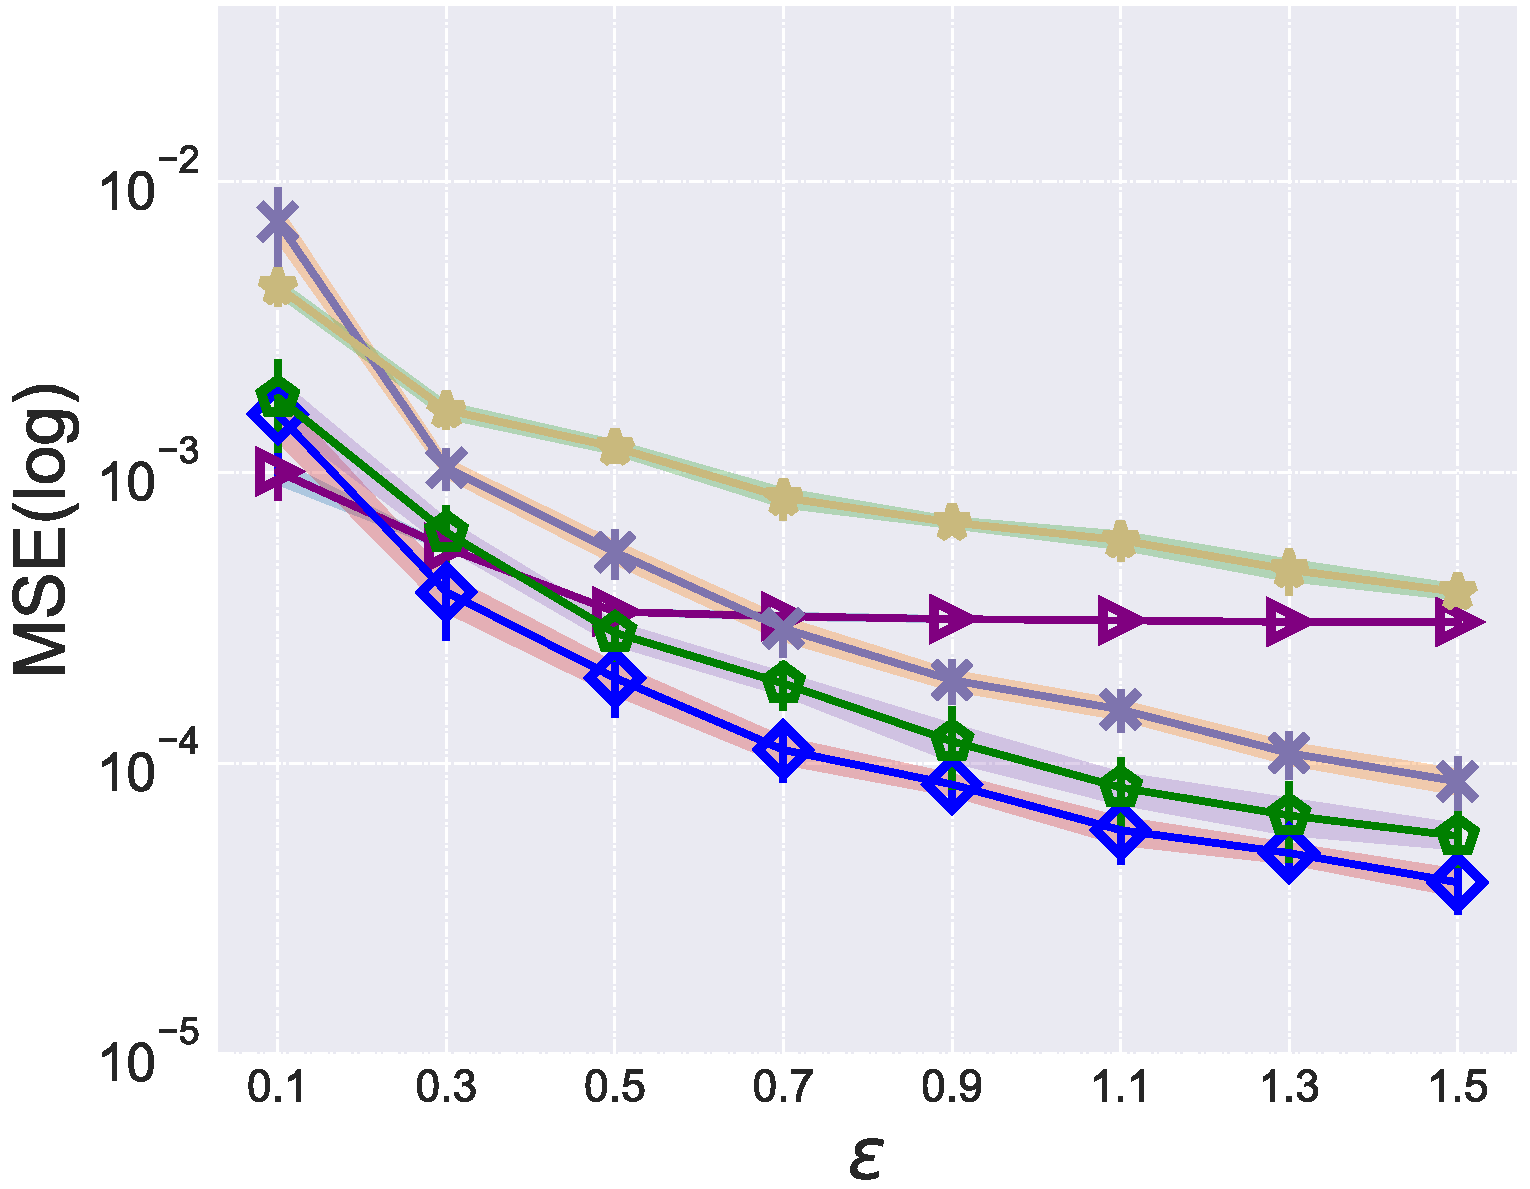
\includegraphics[width=0.24\hsize]{figure/ldp_range_query/figures_experiment_result/overall_result/0406_CI_Rand_ep-Three_Normal08-Set_10_7-Domain_6_6_6.pdf.pdf}}
    \subfigure[\Laplacian~(5), $10^6$, vary $\epsilon$]{\label{fig:Five_Laplace08-Set_10_6-Domain_6_6_6_6_6}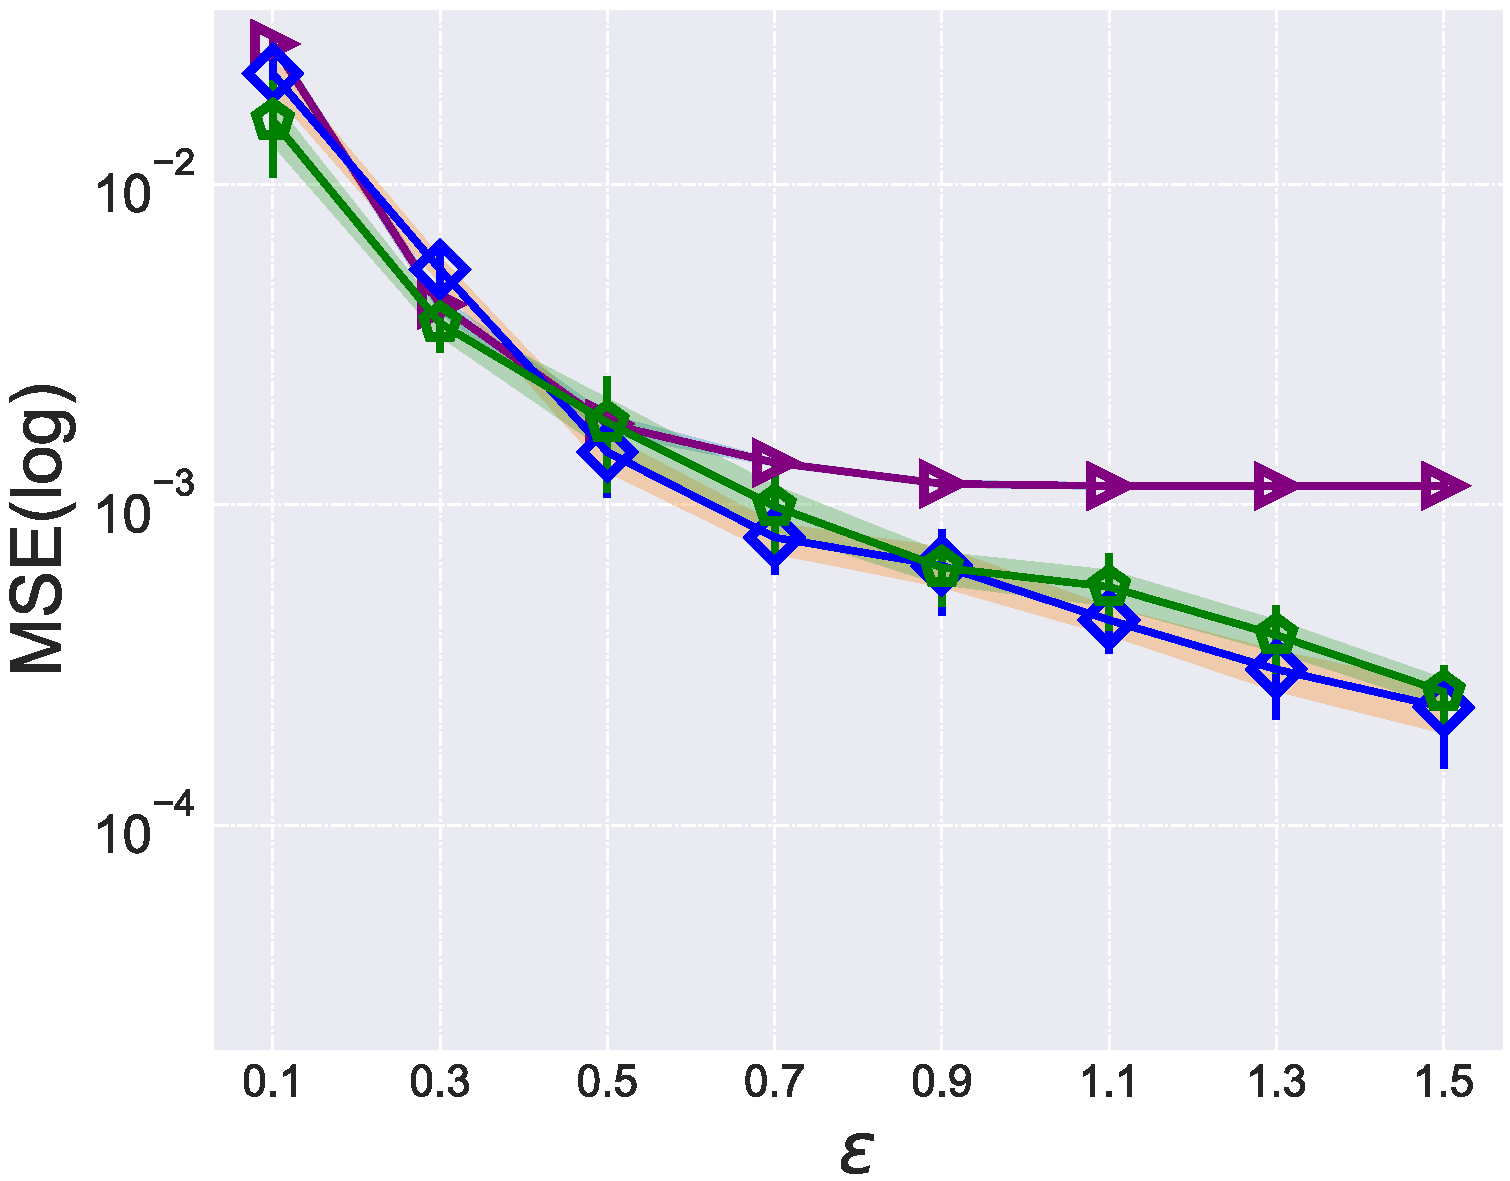
\includegraphics[width=0.24\hsize]{figure/ldp_range_query/figures_experiment_result/overall_result/0406_CI_Rand_ep-Five_Laplace08-Set_10_6-Domain_6_6_6_6_6.pdf.pdf}}
    \subfigure[\Laplacian~(5),$10^7$, vary $\epsilon$]{\label{fig:Five_Laplace08-Set_10_7-Domain_6_6_6_6_6}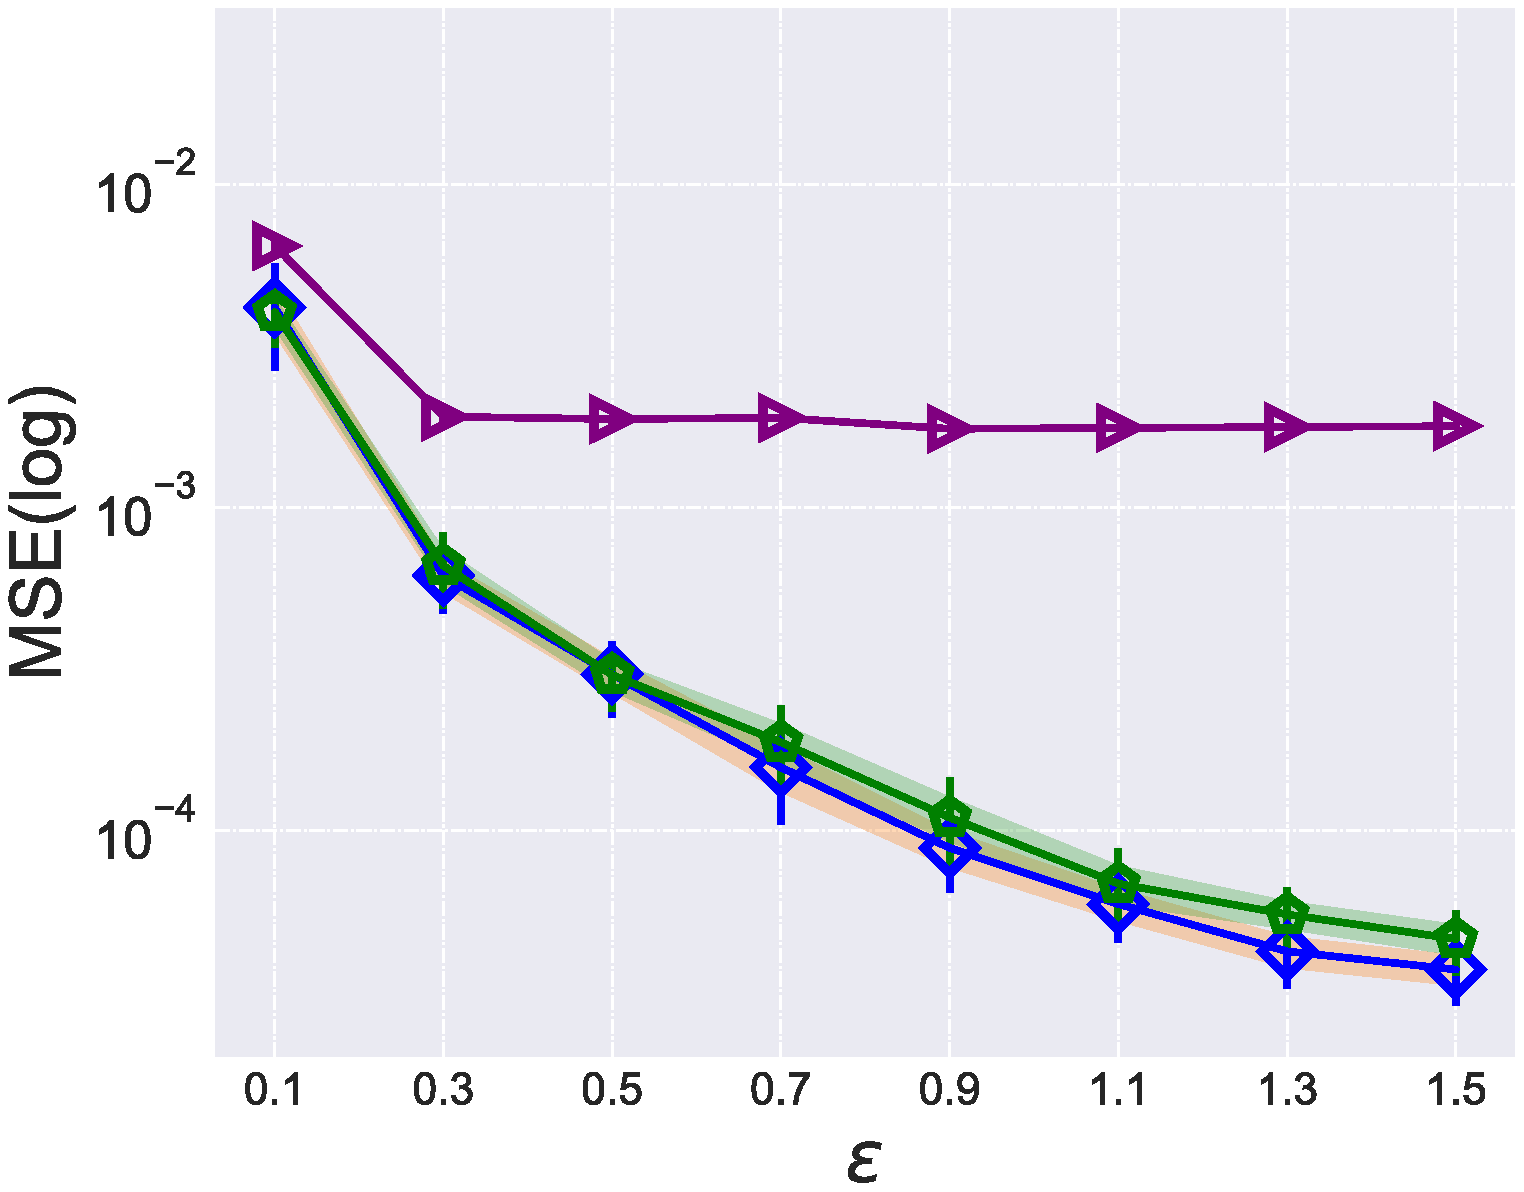
\includegraphics[width=0.24\hsize]{figure/ldp_range_query/figures_experiment_result/overall_result/0406_CI_Rand_ep-Five_Laplace08-Set_10_7-Domain_6_6_6_6_6.pdf.pdf}}
    \subfigure[\Gaussian~(5), $10^6$, vary $\epsilon$]{\label{fig:Five_Normal08-Set_10_6-Domain_6_6_6_6_6}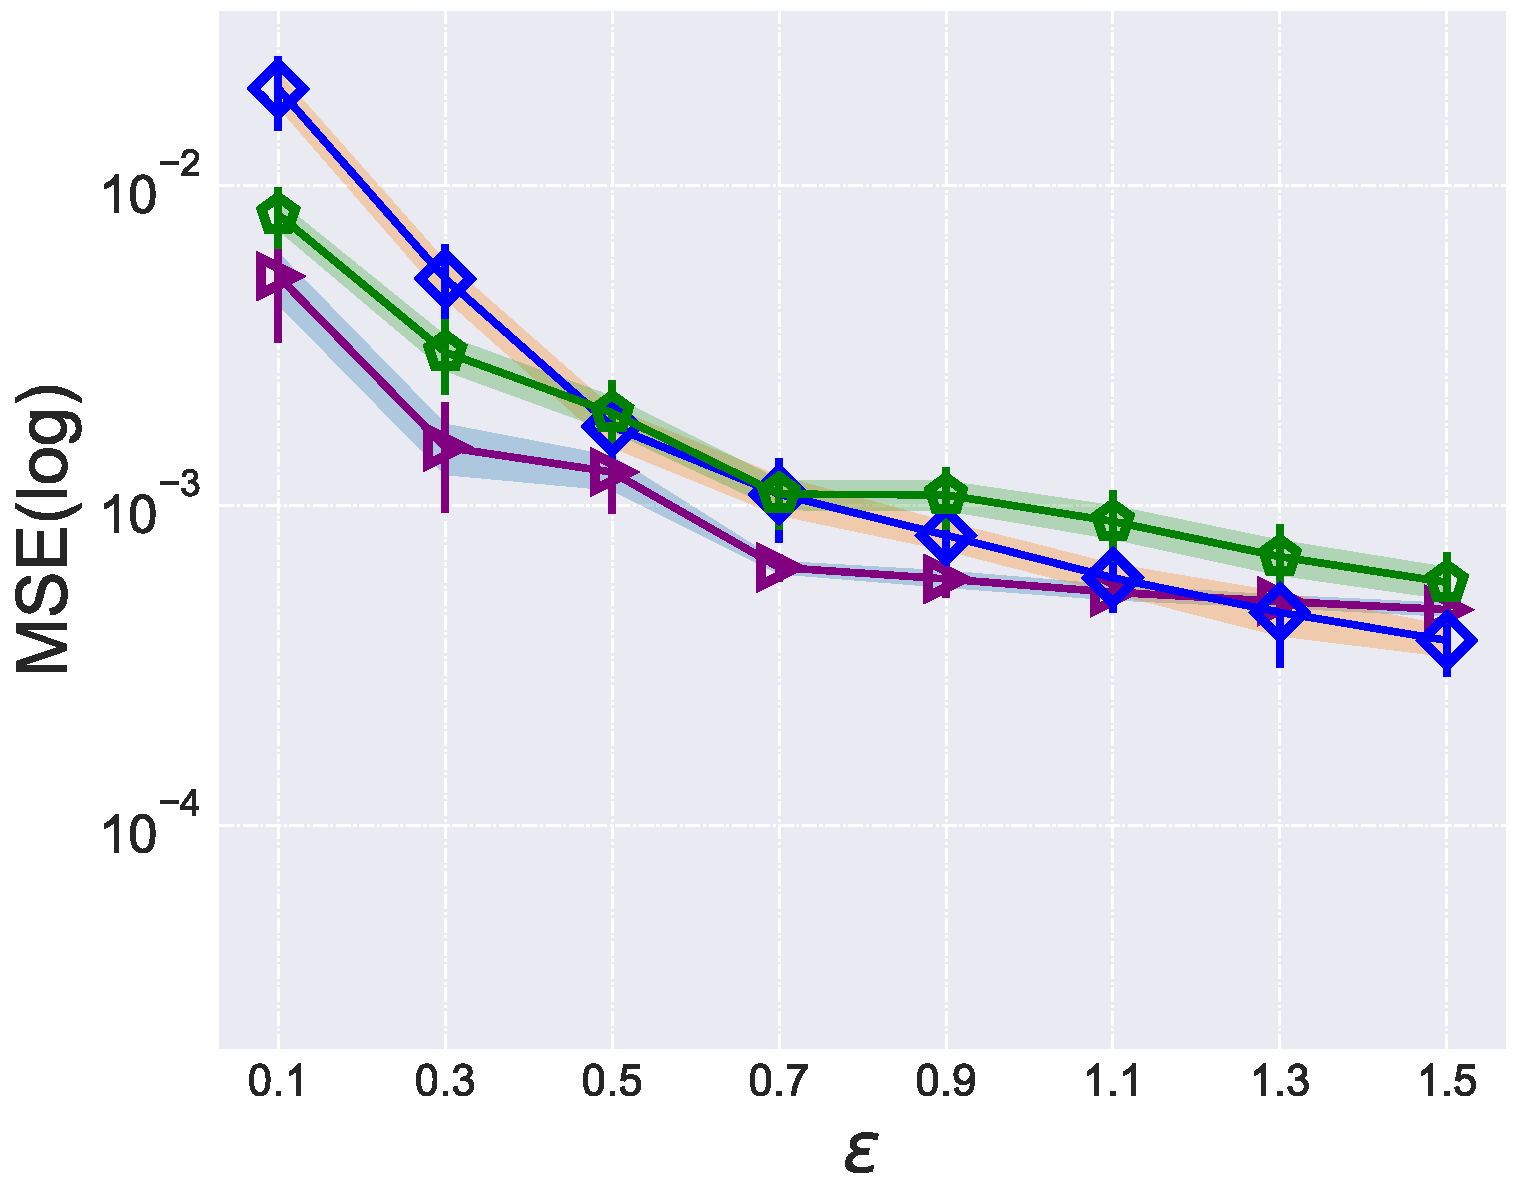
\includegraphics[width=0.24\hsize]{figure/ldp_range_query/figures_experiment_result/overall_result/0406_CI_Rand_ep-Five_Normal08-Set_10_6-Domain_6_6_6_6_6.pdf.pdf}}
    \subfigure[\Gaussian~(5), $10^7$, vary $\epsilon$]{\label{fig:Five_Normal08-Set_10_7-Domain_6_6_6_6_6}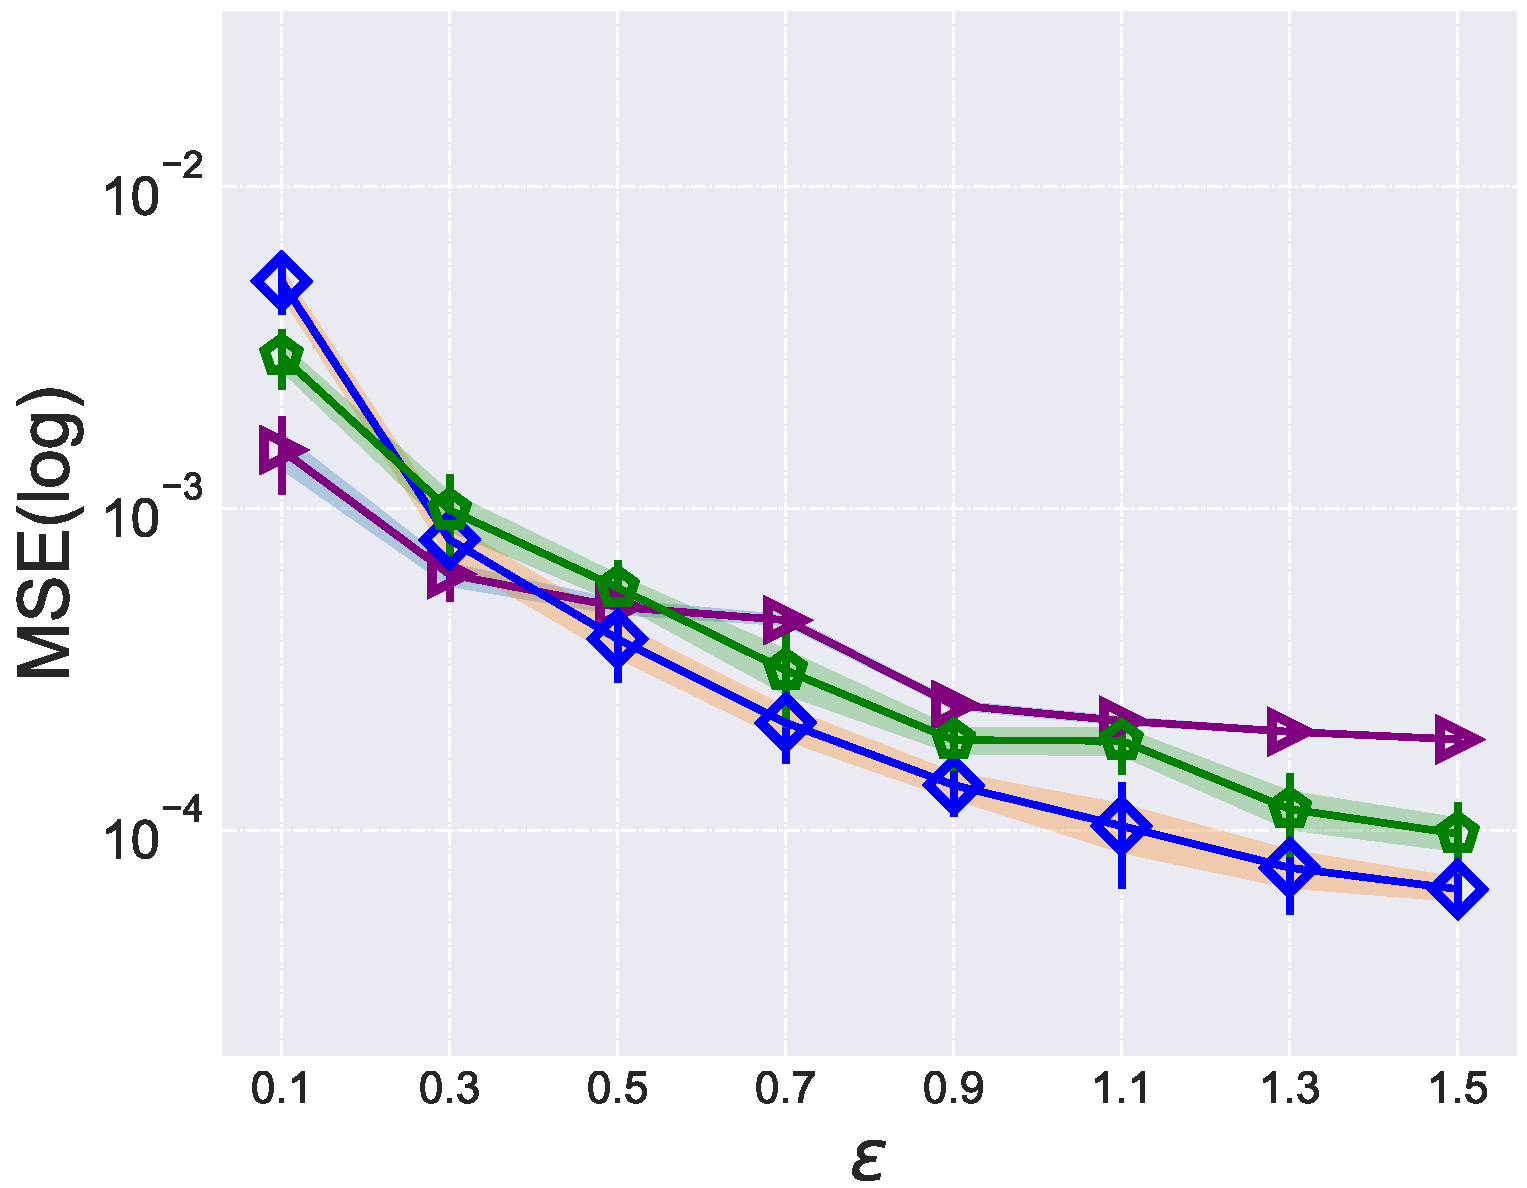
\includegraphics[width=0.24\hsize]{figure/ldp_range_query/figures_experiment_result/overall_result/0406_CI_Rand_ep-Five_Normal08-Set_10_7-Domain_6_6_6_6_6.pdf.pdf}}
    \subfigure{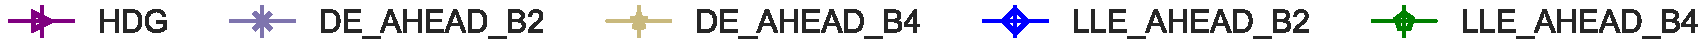
\includegraphics[width=0.85\textwidth]{figure/ldp_range_query/figures_others/comparison_3D_legend5.pdf.pdf}}  
    \vspace{-0.1cm}
    \caption{Comparison of different methods on high-dimensional \Laplacian and \Gaussian datasets under various privacy budgets. \de and \lle respectively represent two high-dimensional expansion methods, \ie, ``direct estimation'' and ``leveraging low-dimensional estimation''. \myHDG is a baseline method. The results are shown in log scale.}
    % \vspace{-0.6cm}
    \label{3,5-dim overall compare}
\end{figure*}

\begin{figure*}[!h]
    \centering
    \subfigure[\Laplacian, $10^6$, $64^m$]{
    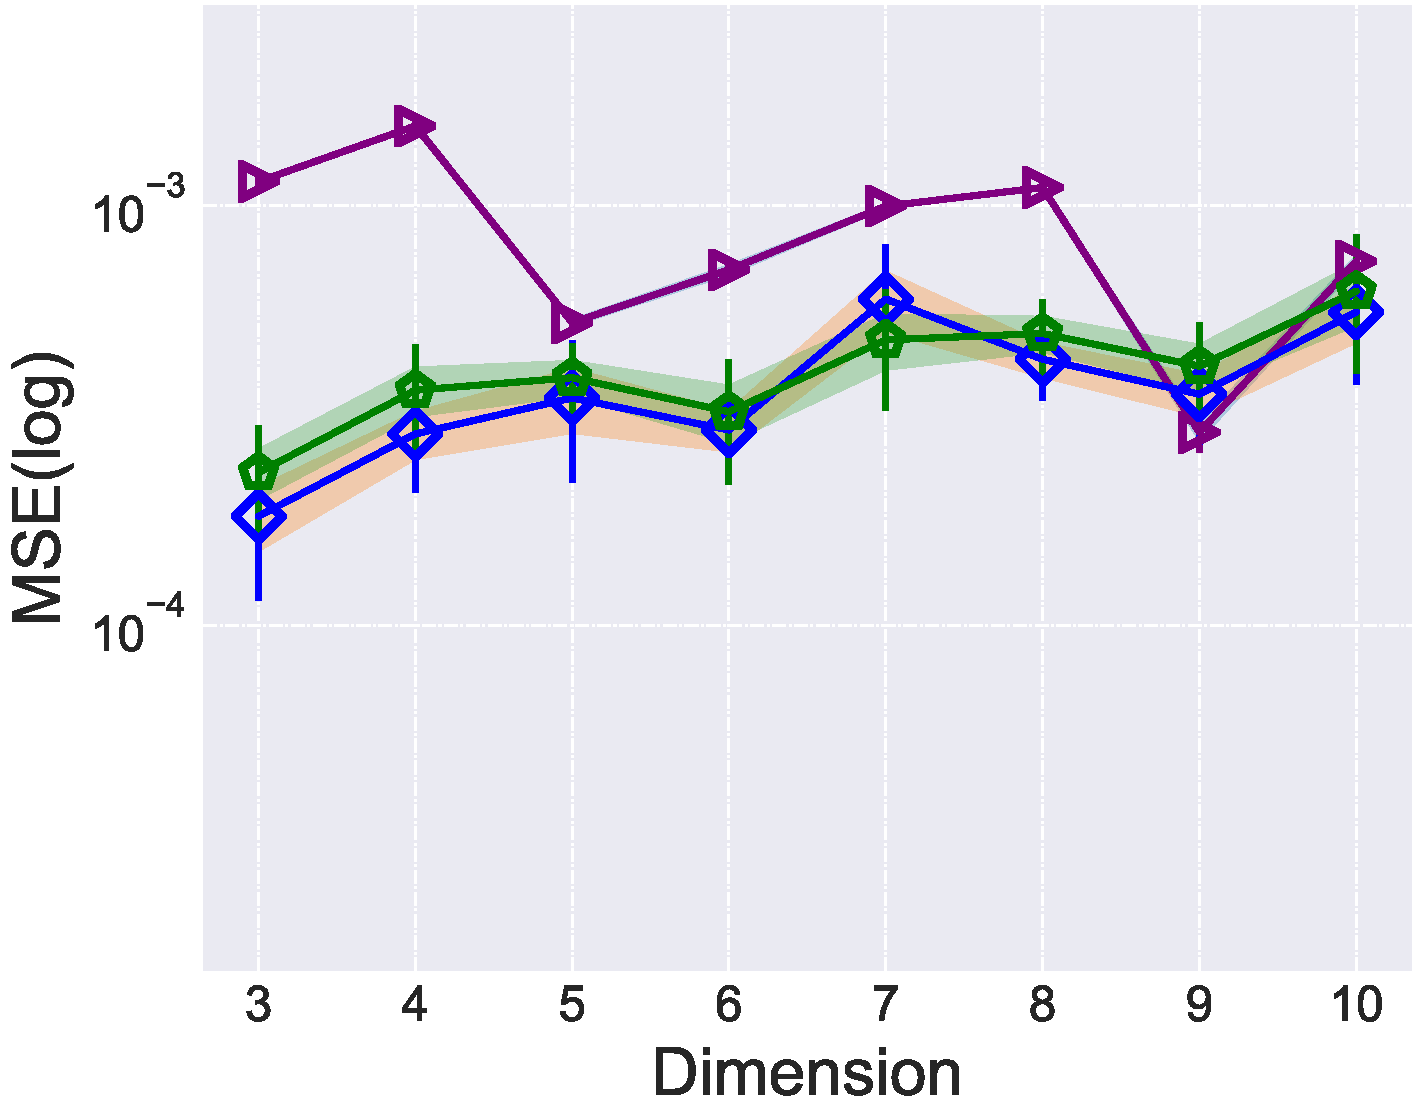
\includegraphics[width=0.23\hsize]{figure/ldp_range_query/figures_experiment_result/various_dimension/0416_CI_Rand-Attribute-Ten_Laplace08-Set_10_6.pdf.pdf}
    \label{fig: Attribute-Ten_Laplace08-Set_10_6}
    }
    \subfigure[\Laplacian, $10^7$, $64^m$]{
    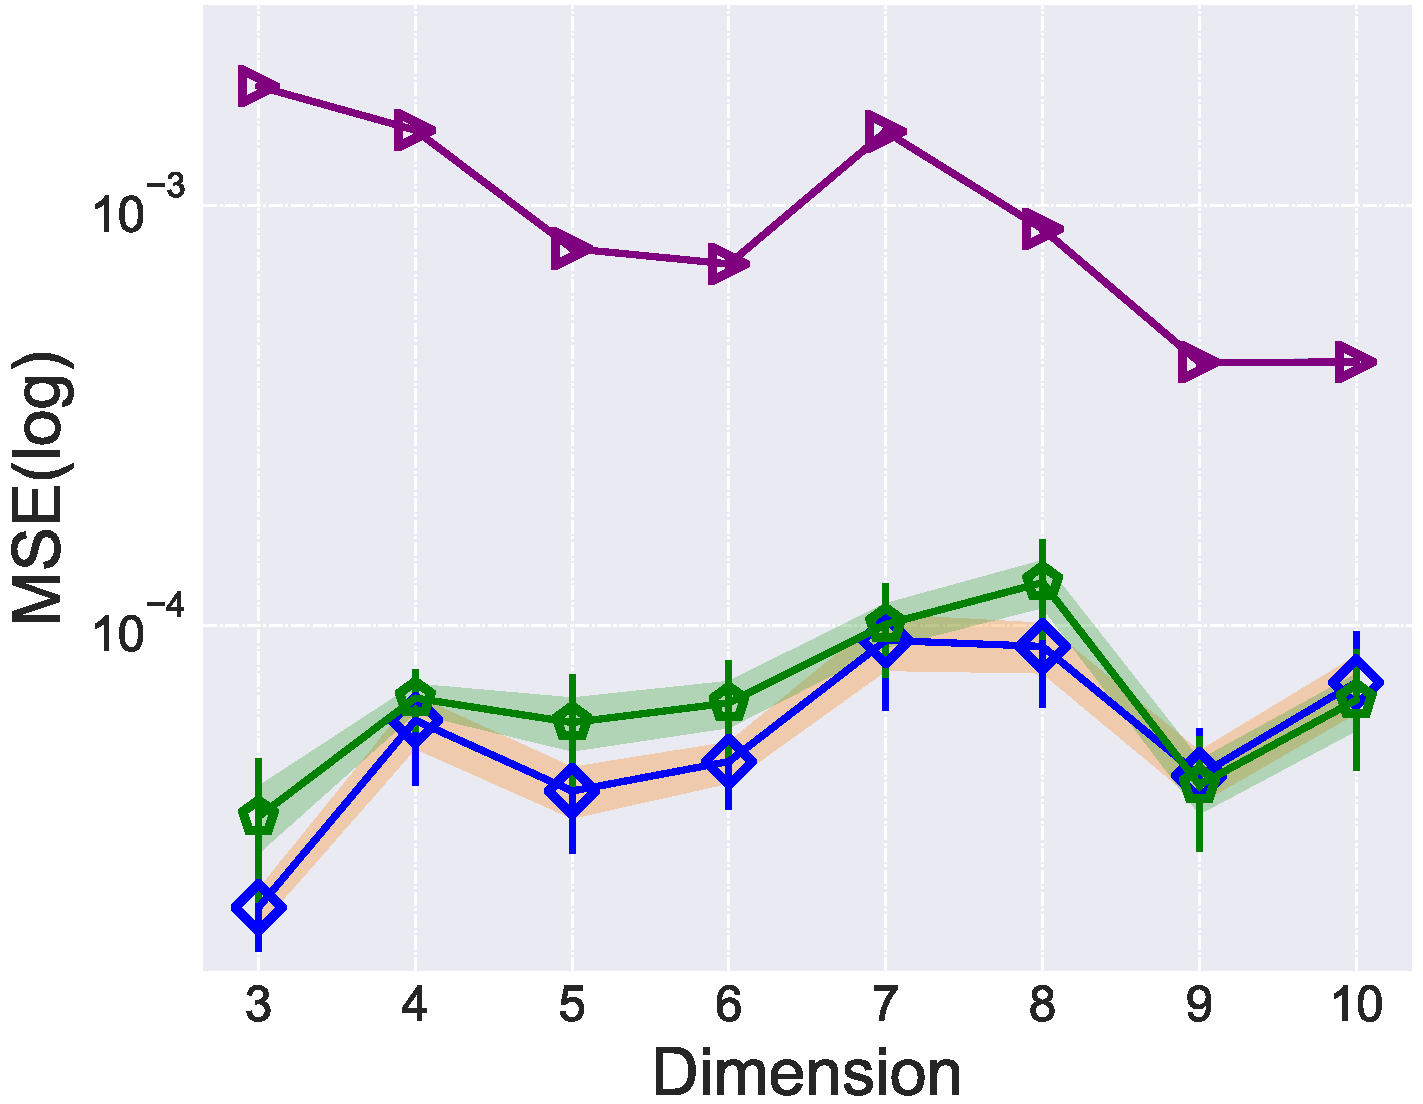
\includegraphics[width=0.23\hsize]{figure/ldp_range_query/figures_experiment_result/various_dimension/0416_CI_Rand-Attribute-Ten_Laplace08-Set_10_7.pdf.pdf}
    \label{fig: Attribute-Ten_Laplace08-Set_10_7}
    }
    \subfigure[\Gaussian, $10^6$, $64^m$]{
    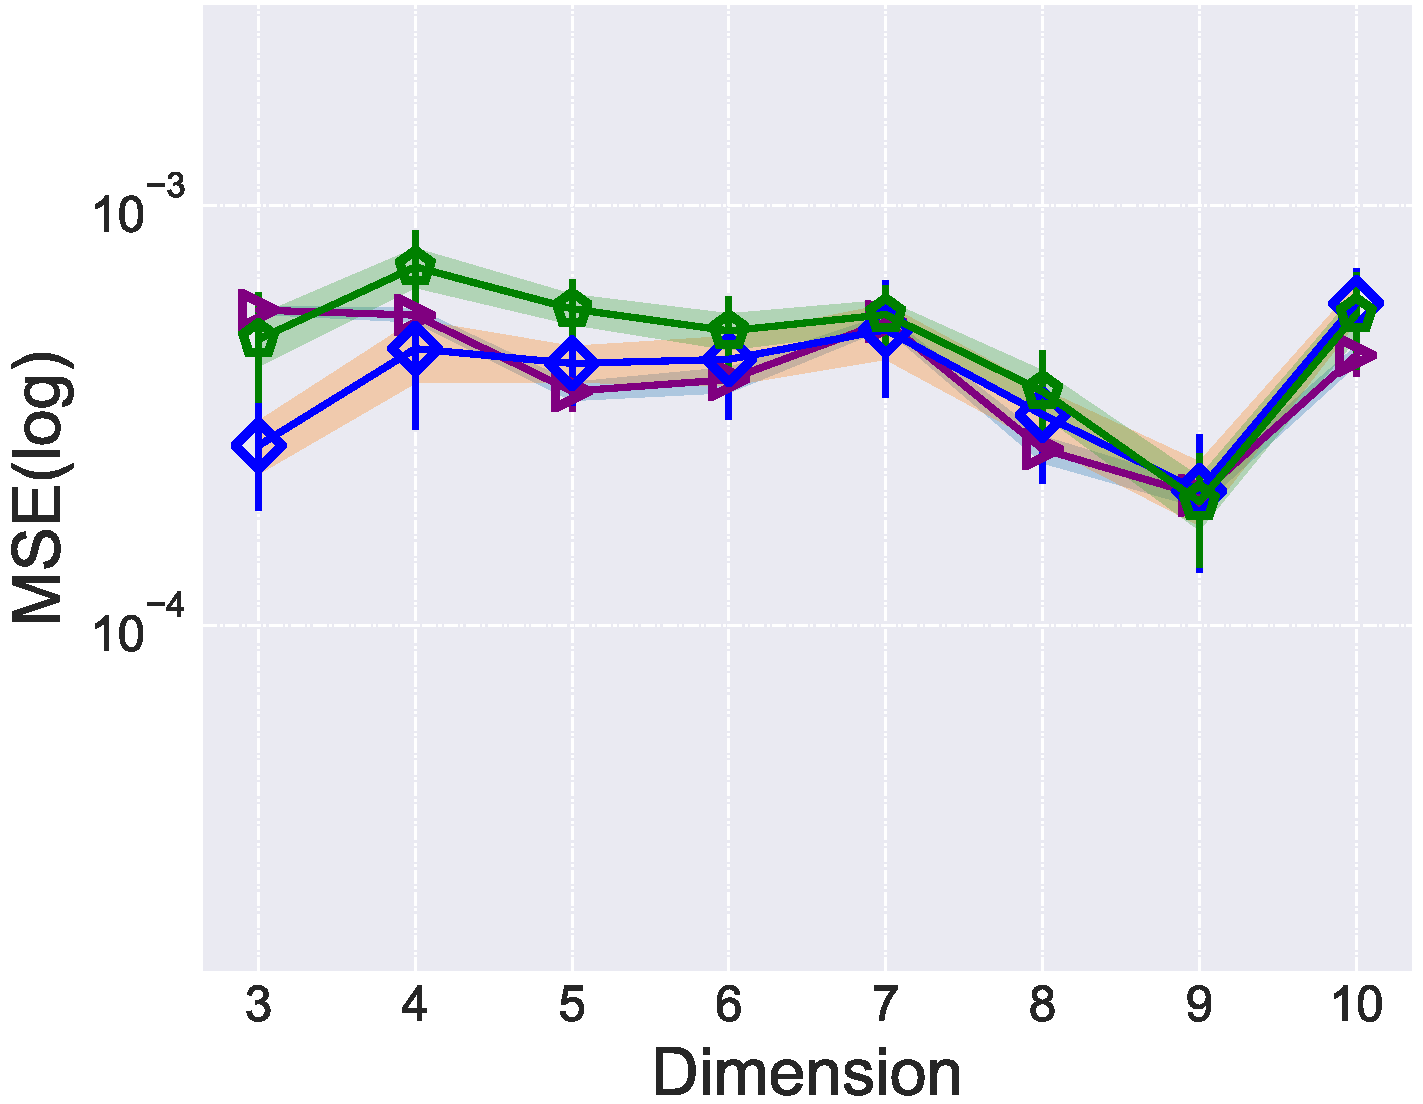
\includegraphics[width=0.23\hsize]{figure/ldp_range_query/figures_experiment_result/various_dimension/0416_CI_Rand-Attribute-Ten_Normal08-Set_10_6.pdf.pdf}
    \label{fig: Attribute-Ten_Normal08-Set_10_6}
    }
    \subfigure[\Gaussian, $10^7$, $64^m$]{
    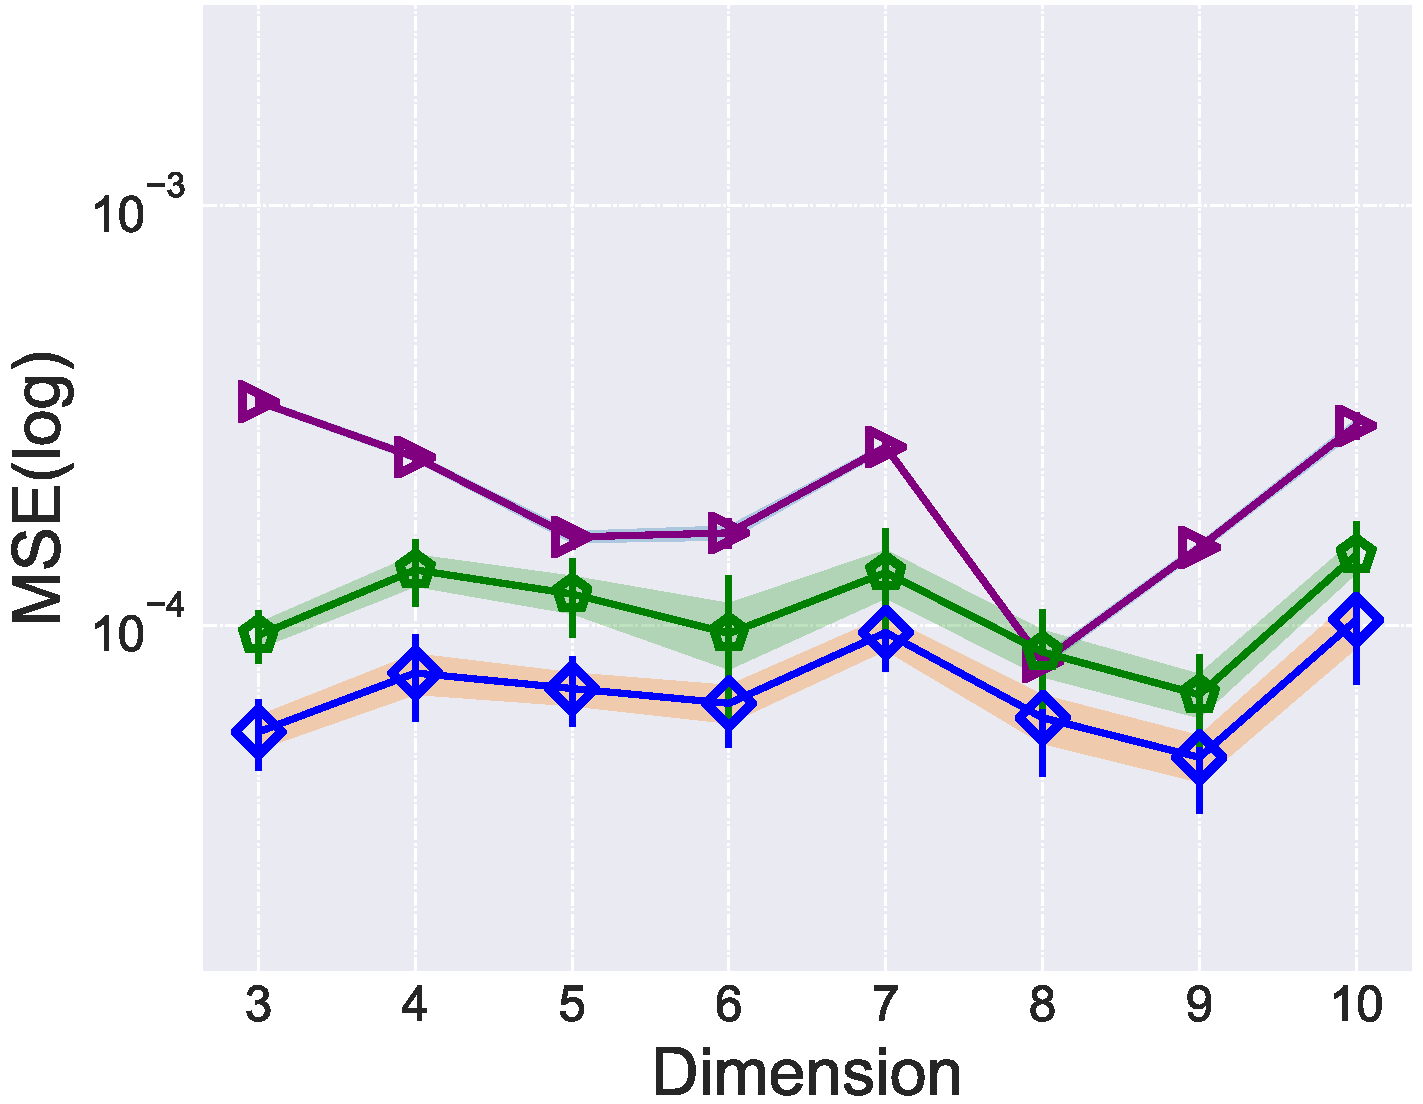
\includegraphics[width=0.23\hsize]{figure/ldp_range_query/figures_experiment_result/various_dimension/0416_CI_Rand-Attribute-Ten_Normal08-Set_10_7.pdf.pdf}
    \label{fig: Attribute-Ten_Normal08-Set_10_7}
    }
    \subfigure{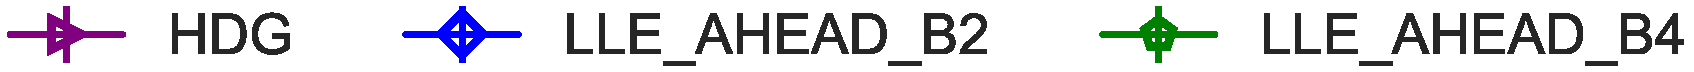
\includegraphics[width=0.55\textwidth]{figure/ldp_range_query/figures_others/comparison_3D_legend3.pdf.pdf}}  
    \vspace{-0.1cm}
    \caption{The MSE of different methods when varying data dimension $m$ with $\epsilon = 1.1$. The results are shown in log scale. }
    % \vspace{-0.4cm}
    \label{fig: varying attribute dimension}
\end{figure*}

在本小节中,我们评估 \myahead 在高维场景下的表现。
基于\autoref{2-dim overall compare}和\autoref{2-dim correlation}的实验结果,\myHDG 和 \myahead 的查询精度对数据域大小不敏感。
因此,我们将数据域大小设置为 $|D|=2^6$ ,
并分别从高维 \Laplacian 和 \Gaussian 分布中采样 $10^6$ 和 $10^7$ 条记录的合成数据集进行实验。

\mypara{两种不同高维场景的扩展方法}

% 由于篇幅限制,我们将读者引至 \autoref{High-dimensional Range Query on Real datasets} 中,以获取对 \myahead 在高维真实数据集上的评估。








\section{本章小结}





















% \begin{figure}[htbp]
%     \centering
%     \includegraphics[width=.3\linewidth]{example-image-a}
%     \caption{\label{fig:fig-placeholder}图片占位符}
% \end{figure}

\chapter{再一章}

\par 如\autoref{alg:sample},这是一个算法

\begin{algorithm}[H]
    \begin{algorithmic} % enter the algorithmic environment
        \REQUIRE $n \geq 0 \vee x \neq 0$
        \ENSURE $y = x^n$
        \STATE $y \Leftarrow 1$
        \IF{$n < 0$}
            \STATE $X \Leftarrow 1 / x$
            \STATE $N \Leftarrow -n$
        \ELSE
            \STATE $X \Leftarrow x$
            \STATE $N \Leftarrow n$
        \ENDIF
        \WHILE{$N \neq 0$}
            \IF{$N$ is even}
                \STATE $X \Leftarrow X \times X$
                \STATE $N \Leftarrow N / 2$
            \ELSE[$N$ is odd]
                \STATE $y \Leftarrow y \times X$
                \STATE $N \Leftarrow N - 1$
            \ENDIF
        \ENDWHILE
    \end{algorithmic}
    \caption{\label{alg:sample}算法样例}
\end{algorithm}


